% Template for the submission to:
%   The Annals of Applied Statistics    [AOAS]
%
%%%%%%%%%%%%%%%%%%%%%%%%%%%%%%%%%%%%%%%%%%%%%%
%% In this template, the places where you   %%
%% need to fill in your information are     %%
%% indicated by '???'.                      %%
%%                                          %%
%% Please do not use \input{...} to include %%
%% other tex files. Submit your LaTeX       %%
%% manuscript as one .tex document.         %%
%%%%%%%%%%%%%%%%%%%%%%%%%%%%%%%%%%%%%%%%%%%%%%

\documentclass[aoas]{imsart}

%% Packages
\RequirePackage{amsthm,amsmath,amsfonts,amssymb,centernot,float,import,makeidx,subfiles, mathtools, epstopdf, hyperref, lscape, subcaption, accents, tabularx, threeparttable, varioref, longtable, natbib, graphicx}
%\RequirePackage{natbib}
%\RequirePackage[colorlinks,citecolor=blue,urlcolor=blue]{hyperref}
%\RequirePackage{graphicx}% uncomment this for including figures
%\usepackage{subcaption}
%\usepackage{accents}
%\usepackage{threeparttable}
\usepackage[nokeyprefix]{refstyle}
%\usepackage{varioref}
\startlocaldefs
%%%%%%%%%%%%%%%%%%%%%%%%%%%%%%%%%%%%%%%%%%%%%%
%%                                          %%
%% Uncomment next line to change            %%
%% the type of equation numbering           %%
%%                                          %%
%%%%%%%%%%%%%%%%%%%%%%%%%%%%%%%%%%%%%%%%%%%%%%
%\numberwithin{equation}{section}
%%%%%%%%%%%%%%%%%%%%%%%%%%%%%%%%%%%%%%%%%%%%%%
%%                                          %%
%% For Axiom, Claim, Corollary, Hypothezis, %%
%% Lemma, Theorem, Proposition              %%
%% use \theoremstyle{plain}                 %%
%%                                          %%
%%%%%%%%%%%%%%%%%%%%%%%%%%%%%%%%%%%%%%%%%%%%%%
%%%%%%%%%%%%%%%%%%%%%%%%%%%%%%%%%%%%%%%%%%%%%%
\theoremstyle{plain}
\newtheorem{axiom}{Axiom}
\newtheorem{claim}[axiom]{Claim}
\newtheorem{theorem}{Theorem}[section]
\newtheorem{lemma}[theorem]{Lemma}
\newtheorem{proposition}{Proposition}
\newcommand{\matr}[1]{\mathbf{#1}} % undergraduate algebra version
\newcommand{\mathbbm}[1]{\text{\usefont{U}{bbm}{m}{n}#1}} 
%%%%%%%%%%%%%%%%%%%%%%%%%%%%%%%%%%%%%%%%%%%%%%
%%                                          %%
%% For Assumption, Definition, Example,     %%
%% Notation, Property, Remark, Fact         %%
%% use \theoremstyle{remark}                %%
%%                                          %%
%%%%%%%%%%%%%%%%%%%%%%%%%%%%%%%%%%%%%%%%%%%%%%
\theoremstyle{remark}
\newtheorem{remark}{remark}
%%%%%%%%%%%%%%%%%%%%%%%%%%%%%%%%%%%%%%%%%%%%
%\theoremstyle{plain}
%\newtheorem{???}{???}
%\newtheorem*{???}{???}
%\newtheorem{???}{???}[???]
%\newtheorem{???}[???]{???}
%%%%%%%%%%%%%%%%%%%%%%%%%%%%%%%%%%%%%%%%%%%%%%
%%                                          %%
%% For Assumption, Definition, Example,     %%
%% Notation, Property, Remark, Fact         %%
%% use \theoremstyle{remark}                %%
%%                                          %%
%%%%%%%%%%%%%%%%%%%%%%%%%%%%%%%%%%%%%%%%%%%%%%
%\theoremstyle{remark}
%\newtheorem{???}{???}
%\newtheorem*{???}{???}
%\newtheorem{???}{???}[???]
%\newtheorem{???}[???]{???}
%%%%%%%%%%%%%%%%%%%%%%%%%%%%%%%%%%%%%%%%%%%%%%
%% Please put your definitions here:        %%
%%%%%%%%%%%%%%%%%%%%%%%%%%%%%%%%%%%%%%%%%%%%%%
\endlocaldefs

% reference external document
\makeatletter
\newcommand*{\addFileDependency}[1]{
  \typeout{(#1)}
  \@addtofilelist{#1}
  \IfFileExists{#1}{}{\typeout{No file #1.}}
}
\makeatother

\newcommand*{\myexternaldocument}[1]{
    \externaldocument{#1}
    \addFileDependency{#1.tex}
    \addFileDependency{#1.aux}
}
%%% END HELPER CODE

% put all the external documents here!

\begin{document}

\begin{frontmatter}
%%%%%%%%%%%%%%%%%%%%%%%%%%%%%%%%%%%%%%%%%%%%%%
%%                                          %%
%% Enter the title of your article here     %%
%%                                          %%
%%%%%%%%%%%%%%%%%%%%%%%%%%%%%%%%%%%%%%%%%%%%%%
\title{Balancing weights for region-level analysis: the effect of Medicaid Expansion on the uninsurance rate among states that did not expand Medicaid}
%\title{A sample article title with some additional note\thanksref{T1}}
\runtitle{Medicaid Expansion}
%\thankstext{T1}{A sample of additional note to the title.}

\begin{aug}
\author[A]{\fnms{Max} \snm{Rubinstein}\ead[label = e1]{mrubinst@andrew.cmu.edu}},
\author[A]{\fnms{Amelia} \snm{Haviland}\ead[label = e2,mark]{amelia@andrew.cmu.edu}}, \and
\author[A]{\fnms{David} \snm{Choi}\ead[label = e3,mark]{davidch@andrew.cmu.edu}}
\address[A]{Carnegie Mellon University, Heinz College and Department of Statistics \& Data Science, \printead{e1,e2,e3}}
\end{aug}

\begin{flushleft}
We predict the average effect of Medicaid expansion on the non-elderly adult uninsurance rate among states that did not expand Medicaid in 2014 as if they had expanded their Medicaid eligibility requirements. Using American Community Survey data aggregated to the region level, we estimate this effect by finding weights that approximately reweights the expansion regions to match the covariate distribution of the non-expansion regions. Existing methods to estimate balancing weights often assume that the covariates are measured without error and do not account for dependencies in the outcome model. Our covariates have random noise that is uncorrelated with the outcome errors and our outcome model has state-level random effects inducing dependence between regions. To correct for the bias induced by the measurement error, we propose generating our weights on a linear approximation to the true covariates, using an idea from measurement error literature known as ``regression-calibration'' (see, e.g., \cite{carroll2006measurement}). This requires auxiliary data to estimate the variability of the measurement error. We also modify the Stable Balancing Weights objective proposed by \cite{zubizarreta2015stable}) to reduce the variance of our estimator when the model errors follow our assumed correlation structure. We show that these approaches outperform existing methods when attempting to predict observed outcomes during the pre-treatment period. Using this method we estimate that Medicaid expansion would have caused a -2.33 (-3.54, -1.11) percentage point change in the adult uninsurance rate among states that did not expand Medicaid.
\end{flushleft}


\begin{keyword}
\kwd{Medicaid expansion}
\kwd{balancing weights}
\kwd{measurement error}
\kwd{hierarchical data}
\end{keyword}

\end{frontmatter}
%%%%%%%%%%%%%%%%%%%%%%%%%%%%%%%%%%%%%%%%%%%%%%
%% Please use \tableofcontents for articles %%
%% with 50 pages and more                   %%
%%%%%%%%%%%%%%%%%%%%%%%%%%%%%%%%%%%%%%%%%%%%%%
%\tableofcontents

%%%%%%%%%%%%%%%%%%%%%%%%%%%%%%%%%%%%%%%%%%%%%%
%%%% Main text entry area:

\section{Introduction}

We study the effect of 2014 Medicaid expansion on the non-elderly adult uninsurance rates among states that did not expand Medicaid in 2014 as if they had expanded their Medicaid eligibility requirements. We use public-use survey microdata from annual American Community Survey (ACS) aggregated to the consistent public use microdata area (CPUMA) level, a geographic region that falls within states. We calculate weights that reweight expansion-state CPUMAs to approximately match the covariate distribution of CPUMAs in states that did not expand Medicaid in 2014. We then estimate our causal effect as the difference in means between the reweighted treated CPUMAs and the observed mean of the non-expansion CPUMAs. A key challenge is that our data consists of estimated covariates. The sampling variability in these estimates is a form of measurement error that may bias effect estimates calculated on the observed data. Additionally, CPUMAs fall within states and share a common policy-making environment. The data-generating process for the outcomes therefore may contain state-level random effects that can increase the variance of standard estimation procedures. Our study contributes to the literature on balancing weights by proposing an approach to address both of these problems. We also contribute to the literature on Medicaid expansion by estimating the foregone coverage gains of Medicaid among states that did not expand Medicaid in 2014, which to our knowledge has not yet been directly estimated.

Approximate balancing weights are an estimation method in causal inference that grew out of the propensity score weighting literature. Rather than iteratively modeling the propensity score until the inverse probability weights achieve a desired level of balance, recent papers propose using optimization methods to generate weights that enforce covariate balance between the treated and control units (see, e.g., \cite{hainmueller2012entropy}, \cite{imai2014covariate}, \cite{zubizarreta2015stable}).\footnote{The proposed methods also borrow ideas from the survey literature, which had proposed similar approaches to adjust sample weights to enforce equality between sample totals and known population totals (see, e.g., \cite{haberman1984adjustment}, \cite{deville1992calibration}, \cite{deville1993generalized}, \cite{sarndal2005estimation}).} From an applied perspective, there are at least four benefits of this approach: first, it does not require iterating propensity score models to generate satisfactory weights. Second, these methods (and propensity score methods generally) do not use the outcomes to determine the weights, mitigating the risk of cherry-picking an outcome model specification to obtain a desired result. Third, these methods can constrain the weights to prevent extrapolation from the data, reducing model dependence \cite{zubizarreta2015stable}. Finally, the estimates are more interpretable: by making the comparison group explicit, it is easy to communicate exactly which units contributed to the counterfactual estimate.

Most proposed methods in this literature assume that the covariates are measured without error. For our application we assume that our covariates are measured with mean-zero additive error. This error could potentially bias standard estimation procedures. As a first contribution, we therefore propose generating our weights as a function of a linear approximation to the true covariate values, using an idea from the measurement error literature known as ``regression-calibration'' (see, e.g., \cite{carroll2006measurement}, \cite{gleser1992importance}). This method requires access to an estimate of the measurement error covariance matrix, which we estimate using the ACS microdata. The theoretic consistency of these estimates also requires several assumptions, including that the covariate measurement errors are uncorrelated with any errors in the outcome model, the outcome model is linear, and the data are gaussian. The first assumption is reasonable for our application since the covariates are measured on a different cross-sectional survey than our outcomes. The second is strong but somewhat relaxed because we prevent our weights from extrapolating beyond the support of the data. The third can be relaxed to obtain consistent estimates using ordinary least squares (OLS), but unfortunately not with our proposed method. Despite appearing costly, we show in Section~\ref{ssec:methodsmsrment} that this tradeoff is likely worth it in our application.

As a second contribution, we propose modifying the Stable Balancing Weights (SBW) objective (\cite{zubizarreta2015stable}) to account for possible state-level dependencies in our outcome model. We assume that the errors are homoskedastic with constant positive equicorrelation, though our general approach can accommodate other assumed correlation structures. In a setting without measurement error, we show that this modification can reduce the variance of the resulting estimates. We also connect these weights to the implied regression weights from Generalized Least Squares (GLS). Our overall approach provides a general framework that can be used by other applied researchers who wish to use balancing weights to estimate causal effects when their data are measured with error and/or the model errors are dependent.\footnote{Our approach also relates to the ``synthetic controls'' literature (see, e.g., \cite{abadie2010synthetic}). Synthetic controls are a popular balancing weights approach frequently used in the applied economics literature to estimate treatment effects on the treated (ETT) for region-level policy changes when using time series cross sectional data. Our application uses a similar data structure; however, we instead consider the problem of estimating the ETC. In contrast to much of the synthetic controls literature, which assumes that the counterfactual outcomes follow a linear factor model, we also assume no unmeasured confounding and a linear outcome model.}

Section 2 begins with a more detailed overview of the policy problem, and then defines the study period, covariates, outcome, and treatment. Section 3 discusses our methods, including outlining our identification, estimation, and inferential procedures. Section 4 presents our results. Section 5 contains a discussion of our findings, and Section 6 contains a brief summary. The Appendices contain proofs, summary statistics, and additional results.

\section{Policy Problem and Data}

\subsection{Policy Problem Statement}

Under the Affordable Care Act (ACA), states were required to expand their Medicaid eligibility requirements by 2014 to offer coverage to all adults with incomes at or below 138 percent of the federal poverty level (FPL). The United States Supreme Court ruled this requirement unconstitutional in 2012, allowing states to decide whether to expand Medicaid coverage. In 2014, twenty-six states and the District of Columbia expanded their Medicaid programs. From 2015 through 2020, an additional twelve states elected to expand their Medicaid programs. In July 2021, Oklahoma and Missouri voted to expand their programs.\footnote{https://www.kansascity.com/news/politics-government/article250170945.html} Legislatures in other traditionally conservative states, including Alabama, North Carolina, and Wyoming also reportedly were considering expanding their programs in Spring 2021.\footnote{https://www.nbcnews.com/politics/politics-news/changed-hearts-minds-biden-s-funding-offer-shifts-medicaid-expansion-n1262229} The effects of Medicaid expansion on various outcomes, including uninsurance rates, mortality rates, and emergency department use, have been widely studied, primarily by using the initial expansions in 2014 and 2015 to define expansion states as ``treated'' states and non-expansion states as ``control'' states (see, e.g., \cite{courtemanche2017early}, \cite{wherry2016early}, \cite{ladhania2021effect}).

Medicaid enrollment is not automatic, and take-up rates have historically varied across states. This variation is partly a function of state discretion in administering programs: for example, program outreach, citizenship verification policies, and application processes differ across states (\cite{courtemanche2017early}). Estimating how Medicaid eligibility expansion actually affects the number of uninsured individuals is therefore not obvious. This is also important because many effects are mediated largely through reducing the number of uninsured individuals. Existing studies have estimated that Medicaid expansion reduced the uninsurance rate between three and six percentage points on average among states that expanded Medicaid. These estimates differed depending on the data used, specific target population, study design, and level of analysis (see, e.g., \cite{kaestner2017effects}, \cite{courtemanche2017early}, \cite{frean2017premium}). However, none of these studies have directly estimated the average treatment effect on the controls (ETC). 

We believe that the ETC may differ from the ETT. Every state had different coverage policies prior to 2014, and non-expansion states tended to have less generous policies than expansion states. ``Medicaid expansion'' therefore represents a set of treatments of varying intensities that are distributed unevenly across expansion and non-expansion states. Averaged over the non-expansion states, which tended to have less generous policies and higher uninsurance rates prior to Medicaid expansion, we might expect the average effect to be larger in absolute magnitude than among the expansion states, where ``Medicaid expansion'' on average reflected smaller policy changes.\footnote{As a part of our analysis strategy, we limit our pool of expansion states to those where the policy changes were comparable to the non-expansion states. We also control for pre-treatment uninsurance rates (see Section~\ref{sssec:txassign}).} Even limited to states with equivalent coverage policies prior to 2014 we still might expect the ETT to differ from the ETC. For example, all states that were entirely controlled by the Democratic Party at the executive and legislative levels expanded their Medicaid programs, while only states where the Republican Party controlled at least part of the state government failed to expand their programs. Prior to the 2014 Medicaid expansion, \cite{sommers2012understanding} found that conservative governance was associated with lower Medicaid take-up rates. This might reflect differences in program implementation, which could serve as effect modifiers for comparable policy changes.\footnote{Interestingly, \cite{sommers2012understanding} also find that the association between conservative governance and lower take-up rates prior to 2014 existed even after controlling for a variety of factors pertaining to state-level policy administration decisions. They posit that this may reflect cultural conservatism: people in conservative states are more likely to view enrollment in social welfare programs negatively, and therefore be less likely to enroll.} These factors may then attenuate the effects of Medicaid expansion averaged over non-expansion states relative to expansion states.

The ETC is also interesting in its own right: to the extent the goal of studying Medicaid expansion is to understand the foregone benefits (or potential harms) of Medicaid among non-expansion states, the ETC is the relevant quantity of interest. Authors have previously made claims about the ETC without directly estimating it. For example, \cite{miller2019medicaid} use their estimates of the ETT to predict that had non-expansion states expanded Medicaid, they would have seen 15,000 fewer deaths during their study period. From a policy analysis perspective, we emphasize that researchers should estimate the ETC directly when it answers a substantive question of interest. We therefore contribute to the literature on Medicaid expansion by directly estimating this quantity.

\subsection{Data Source and Study Period}\label{ssec:data}

Our primary data source is the annual household and person public use microdata files from the ACS from 2011 through 2014. The ACS is an annual cross-sectional survey of approximately three million individuals across the United States. The public use microdata files include information on individuals in geographic areas greater than 65,000 people. The smallest geographic unit contained in these data are public-use microdata areas (PUMAs), arbitrary boundaries that nest within states but not within counties or other more commonly used geographic units. One limitation of these data is a 2012 change in the PUMA boundaries, which do not overlap well with the previous boundaries. As a result, the smallest possible geographic areas that nest both PUMA coding systems are known as consistent PUMAs (CPUMAs). The United States contains 1,075 total CPUMAs, with states ranging from having one CPUMA (South Dakota, Montana, and Idaho) to 123 CPUMAs (New York). Our primary dataset contains 929 CPUMAs among 46 states (see also Section~\ref{sssec:txassign}). The average total number of sampled individuals per CPUMA across the four years is 1,001; the minimum number of people sampled was 334 and the maximum is 23,990. We aggregate the microdata to the CPUMA level using the survey weights.  

This aggregation naturally raises concerns about measurement error and hierarchy. Any CPUMA-level variable is an estimate, leading to concerns about measurement error. The hierarchical nature of the dataset -- CPUMAs within states -- raises concerns about geographic dependence.

Our study period begins in 2011, following \cite{courtemanche2017early}, who note that several other aspects of the ACA were implemented in 2010 -- including the provision allowing for dependent coverage until age 26 and the elimination of co-payments for preventative care -- and likely induced differential shocks across states. We also restrict our post-treatment period to 2014. We therefore avoid additional assumptions required for identification given that several states expanded Medicaid in 2015, including Indiana, Michigan, and Pennsylvania.

\subsection{Treatment assignment} \label{sssec:txassign}

Reducing the concept of ``Medicaid expansion'' to a binary treatment simplifies a more complex reality. There are at least three reasons to be cautious about this simplification. First, states differed substantially in their Medicaid coverage policies prior to 2014. Given perfect data we might ideally consider Medicaid expansion as a continuous treatment with values proportional to the number of newly eligible individuals. The challenge is correctly identifying newly eligible individuals in the data (see \cite{frean2017premium}, who attempt to address this). Second, \cite{frean2017premium} note that five states (California, Connecticut, Minnesota, New Jersey, and Washington) and the District of Columbia adopted partial limited Medicaid expansions prior to 2014. The ``2014 expansion'' therefore actually occurred in part prior to 2014 for several states.\footnote{\cite{kaestner2017effects} and \cite{courtemanche2017early} also consider Arizona, Colorado, Hawaii, Illinois, Iowa, Maryland, and Oregon to have had early expansions.} Finally, timing is an issue: among the states that expanded Medicaid in 2014, Michigan's expansion did not go into effect until April 2014, while New Hampshire's expansion did not occur until September 2014.

Our primary analysis excludes New York, Vermont, Massachusetts, Delaware, and the District of Columbia from our pool of expansion states because these states had comparable Medicaid coverage policies prior to 2014 and therefore reflect invalid comparisons (\cite{kaestner2017effects}). We also exclude New Hampshire because it did not expand Medicaid until September 2014. While Michigan expanded Medicaid in April 2014, we leave this state in our pool of ``treated'' states. We consider the remaining expansion states, including those with early expansions, as ``treated'' and the non-expansion states, including those that later expanded Medicaid, as ``control'' states. We later consider the sensitivity of our results to these classifications by removing the early expansion states indicated by \cite{frean2017premium}. Our final dataset contains data for 925 CPUMAs, with 414 CPUMAs among 24 non-expansion states and 511 CPUMAs among 21 expansion states. When we exclude the early expansion states, we are left with 292 CPUMAs across 16 expansion states. We provide a complete list of states by Medicaid expansion classification in Appendix~\ref{app:sumstats}.

\subsection{Outcome}

Our outcome is the non-elderly (individuals aged 18-64) adult uninsurance rate in 2014. While take-up among the Medicaid-eligible population is a more natural outcome, we choose the non-elderly adult uninsurance rate for two reasons, one theoretic and one practical. First, Medicaid eligibility post-expansion is likely endogenous: Medicaid expansion may affect an individual's income and poverty levels, which in general define Medicaid eligibility. Second, we can better compare our results with the existing literature, including \cite{courtemanche2017early}, who also use this outcome. One drawback is that the simultaneous adoption of other ACA provisions by all states in 2014 also affects this outcome. As a result, we only attempt to estimate the effect of Medicaid expansion in 2014 in the context of this changing policy environment. We discuss this further in Sections~\ref{ssec:estimand} and ~\ref{ssec:identification}. 

\subsection{Covariates}

We choose our covariates to approximately align with those considered in \cite{courtemanche2017early} and that are likely to be potential confounders. Specifically, using the ACS public use microdata, we calculate the unemployment and uninsurance rates for each CPUMA from 2011 through 2013. We also estimate a variety of demographic characteristics averaged over this same time period, including percent female, white, married, Hispanic ethnicity, foreign-born, disabled, students, and citizens. We estimate the percent in discrete age categories, education attainment categories, income-to-poverty ratio categories, and categories of number of children. Finally, we calculate the average population growth and number of households to adults. We provide a more extensive description of our calculation of these variables in Appendix~\ref{app:adjustmentdetails}.

In addition to the ACS microdata we use 2010 Census data to estimate the percentage living in an urban area for each CPUMA. Lastly, we include three state-level covariates reflecting the partisan composition of each state's government in 2013 using data obtained from the National Conference of State Legislatures (NCSL). These include an indicator for states with a Republican governor, Republican control over the lower legislative chamber, and Republican control over both legislative chambers and the governorship.\footnote{Nebraska is the only state with a unicameral legislature and the legislature is technically non-partisan. We nevertheless classified them as having Republican control of the legislature for this analysis.} 

\section{Methods}\label{sec:methods}

In this section we present our causal estimand, identifying assumptions, estimation strategy, and inferential procedure. Our primary methodological contributions are contained in the subsection on estimation. We begin by outlining notation.

\subsection{Notation}
We let $s$ index states, and $c$ index CPUMAs within states. Let $m$ denote the number of states, $p_s$  the number of CPUMAs in state $s$, and $n = \sum_{s=1}^m p_s$ the total number of CPUMAs. For each state $s$, let $A_s$ denote its treatment assignment according to the discussion given in Section \ref{sssec:txassign}, with $A_s = 1$ indicating treatment and $A_s=0$ indicating control. For each CPUMA $c$ in state $s$, let $Y_{sc}$ denote the outcome of interest, its uninsurance rate in 2014; let $X_{sc}$ denote a q-dimensional covariate vector; and let $A_{sc} = A_{s}$ denote its treatment status. We assume potential outcomes (\cite{rubin2005causal}), defining a CPUMA's potential uninsurance under treatment by $Y^1_{sc}$, and under control by $Y^0_{sc}$. Finally, we let $n_1$ and $n_0$ denote the number of treated and control CPUMAs, and define $m_1$ and $m_0$ analagously for states.

Given a set of covariate vectors or outcomes $\{Z_{sc}: sc = 11, ..., 1p_1, ..., mp_m\}$ indexed over CPUMAs, let $Z_{A=1}$ and $Z_{A=0}$ denote its subsets corresponding to the treated and control units
\[ Z_{A=a} = \{Z_{sc}: A_{sc}=a\}\]
so that, for example, $X_{A=0}$ corresponds to the covariates of the control units. Let $\bar{Z}_a$ (which abbreviates $\bar{Z}_{A=a}$) denote the average over units with treatment assignment $A_{sc} = a$:

\begin{align*}
	\bar{Z}_a & = \frac{1}{n_a} \sum_{sc: A_{sc}=a} Z_{sc}
\end{align*}
so that, for example, $\bar{Y}_0^1$ represents the average potential outcome under treatment for the control units, and $\bar{X}_0$ represents the average covariate values for the control units.

\subsection{Estimand} \label{ssec:estimand}

We define the causal estimand $\psi$

\begin{align} \label{eqn:psi}
    \psi &= n_0^{-1} \sum_{sc: A_{sc}=0} \mathbb{E}\left[ Y_{sc}^1 - Y_{sc}^0 | X_{sc}\right] = \mathbb{E}[\bar{Y}_0^1 - \bar{Y}_0^0 \mid X_{A=0}] \\ 
    &= \psi_0^1 - \psi_0^0
\end{align}
where $\psi_0^a$ denotes the expectation $\mathbb{E}[\bar{Y}_0^a \mid X_{A=0}]$. The estimand $\psi$ represents the expected treatment effect on non-expansion states conditioning on the observed covariate distribution of the non-expansion states (see, e.g., \cite{imbens2004nonparametric}). The challenge is that we do not observe the counterfactual outcomes for non-expansion CPUMAs had their states expanded their Medicaid programs. We therefore require causal assumptions to identify this counterfactual quantity using our observed data.\footnote{As noted previously, the 2014 Medicaid expansion occurred simultaneously with the implementation of several other major ACA provisions, including (but not limited to) the creation of the ACA-marketplace exchanges, the individual mandate, health insurance subsidies, and community-rating and guaranteed issue of insurance plans (\cite{courtemanche2017early}). Almost all states broadly implemented these reforms beginning January 2014. Conceptually we think of the other ACA components as a state-level treatment ($R$) separate from Medicaid expansion ($A$). Our total estimated effect may also include interactions between these policy changes; however, we do not attempt to separately identify these effects. Without further assumptions, we therefore cannot generalize these results beyond 2014.} 

\subsection{Identification} \label{ssec:identification}

We appeal to the following causal assumptions to identify $\psi$ from our observed data: the stable unit treatment value assumption (SUTVA), no unmeasured confounding given the true covariates and outcome values, and no anticipatory treatment effects. We also invoke parametric assumptions to model the measurement error and to express our estimand in terms of parameters from a linear model. We conclude by using ideas from the ``regression-calibration'' literature (\cite{gleser1992importance}) to ensure that identifying our target estimand is possible given auxiliary data on the measurement error covariance matrix.

We first assume the SUTVA at the CPUMA level. Assuming the SUTVA has two implications for our analysis: first, that there is only one version of treatment; second, that each unit's potential outcome only depends on its treatment assignment. We discussed potential violations of the first implication previously when considering how to reduce Medicaid expansion to a binary treatment. The second implication could be violated if one CPUMA's expansion decision affected uninsurance rates in another CPUMA (see, e.g., \cite{frean2017premium}). On the other hand, our assumption allows for interference among individuals living within CPUMAs and is therefore weaker than assuming no interference among any individuals. Further addressing this is beyond the scope of this paper.

Second, we assume no effects of treatment on the observed covariates. This includes assuming no anticipatory effects on pre-2014 uninsurance rates. This is violated in our study, as some treated states allowed early Medicaid expansion for specific counties, affecting their pre-2014 uninsurance rates. We later test the sensitivity of our results to the exclusion of these states.

Third, we assume no unmeasured confounding. Specifically, we posit that in 2014 the potential outcomes for each CPUMA are jointly independent of the state-level treatment assignment conditional on CPUMA and state-level covariates $X_{sc}$:

\begin{equation}\label{eqn:unconfoundedness}
(Y_{sc}^1, Y_{sc}^0) \perp A_s \mid X_{sc} 
\end{equation}

The covariate vector $X_{sc}$ includes both time-varying pre-treatment covariates, including pre-treatment outcomes, and covariates averaged across 2011-2013, such as demographic characteristics, and the state-level governance indicators discussed in Section~\ref{ssec:data}. We believe this assumption is reasonable given our rich covariate set. 

Fourth, we assume that the outcomes for each treatment group are linear in the true covariates:

\begin{equation}\label{eqn:linmod}
Y_{sc}^a = \alpha_a + X_{sc}^T\beta_a + \epsilon_{sc} + \varepsilon_s \qquad a = 0, 1
\end{equation}
%
where the errors $\epsilon_{sc}$ and $\varepsilon_{s}$ are mean-zero; independent from the covariates, treatment assignment, and each other; and have finite variances $\sigma^2_{\epsilon}$ and $\sigma^2_{\varepsilon}$, respectively.\footnote{Because our covariates include pre-treatment outcomes, this assumption also implies that $\epsilon_{sc}$ and $\varepsilon_{sc}$ are uncorrelated with pre-treatment outcomes, including any error terms that might appear in their generative models.} This implies that the errors for each CPUMA within a given state have a constant within-state correlation $\frac{\sigma^2_{\varepsilon}}{\sigma^2_{\varepsilon} + \sigma^2_{\epsilon}}$, which we denote as $\rho$. To fix ideas, $\epsilon_{sc}$ may capture time-specific idiosyncracies at the local level, possibly due to the local policy or economic conditions. By contrast $\varepsilon_s$ captures time-specific idiosyncracies at the state-level that are common across CPUMAs within a state due to the shared policy and economic environment.

Fifth, we assume that the covariates $X$ and outcomes $Y$ are not observed directly. Instead, survey sampled versions $W$ and $J$ are available, with additive gaussian measurement error arising due to sample variability.

\begin{align} \label{eqn:additivenoise}
	J_{sc} & = Y_{sc} + \xi_{sc} & \text{and} & & W_{sc} & = X_{sc} + \nu_{sc}
\end{align}
where $(\xi_{sc}, \nu_{sc})$ is independent of $(X, Y)$ and has distribution

\begin{equation} \label{eqn:gaussiannoise}
 (\xi_{sc}, \nu_{sc}) \stackrel{\text{indep}}{\sim} \operatorname{MVN}\left(0, \left[\begin{array}{cc} \sigma_{\xi,sc}^2 & 0 \\ 0 & \Sigma_{\nu, sc} \end{array}\right] \right)
\end{equation}

We believe equations (\ref{eqn:additivenoise}) and (\ref{eqn:gaussiannoise}) are reasonable because measurement error in our context is sampling variability. While \eqref{eqn:gaussiannoise} further implies the measurement errors in our covariates and outcomes are uncorrelated, this is reasonable because our outcomes are measured on a different cross-sectional survey than our covariates.\footnote{Our covariates are almost all ratio estimates, which are in general biased. This bias, however, diminishes quickly with the sample size; given that our sample sizes are all over 300, we treat these estimates as unbiased.} 

Sixth, we assume that the covariates for the treated units $X_{sc}$ are drawn i.i.d. multivariate normal conditional on treatment:

\begin{align} \label{eqn:Xgaussian}
    X_{sc}|A_{sc} = 1 & \stackrel{\text{iid}}{\sim} MVN(\upsilon_1, \Sigma_{X|1})%, \qquad \forall\, sc: A_{sc} = a,
\end{align}
%
Under equations (\ref{eqn:gaussiannoise})-(\ref{eqn:Xgaussian}), the conditional expectation of $X_{sc}$ given noisy observation $W$ among the treated units can be seen to equal 

\begin{equation} \label{eqn:regcal}
\mathbb{E}[X_{sc}| W, A] = \upsilon_1 + \Sigma_{X|1} \left(\Sigma_{X|1} + \Sigma_{\nu, sc}\right)^{-1}  (W_{sc} - \upsilon_1), \qquad \forall\, sc: A_{sc} = 1
\end{equation}
%
Equation (\ref{eqn:Xgaussian}) is a convenient simplification to motivate \eqref{eqn:regcal}. For example, $X_{sc}$ includes state-level covariates, so the covariates cannot be independent. More generally, many of the covariates are bounded, and therefore cannot be gaussian. In fact, assuming (\ref{eqn:Xgaussian}) is not strictly necessary for consistent estimation of $\psi_0^1$ (see, e.g., \cite{gleser1992importance}); however, it is required by the weighting approaches that we consider here. In our validation experiments described in Section~\ref{sec:validation}, we find that approaches that assume (\ref{eqn:Xgaussian}) outperform those that do not, as the latter group evidently relies more heavily on the linearity assumption (\ref{eqn:linmod}).

In principle it may be possible to generalize equations (\ref{eqn:additivenoise})-(\ref{eqn:Xgaussian}) to settings where the conditional expectation $\mathbb{E}[X_{sc}|W,A]$ follows a different form than \eqref{eqn:regcal}, but is still accessible given auxiliary data. For example, to make the linearity assumption of equation (\ref{eqn:linmod}) more credible, $X_{sc}$ might include transformations or a basis expansion of the covariate, so that $X_{sc} = \phi(U_{sc})$ for some function $\phi$ of the untransformed covariates $U_{sc}$. Under assumptions analogous to (\ref{eqn:additivenoise})-(\ref{eqn:Xgaussian}) for $U_{sc}$, we may still be able to estimate $\mathbb{E}[X_{sc} \mid W, A]$. We give some preliminary findings in Appendix \ref{app:AsecI}, Remark \ref{remark:basis expansion}. Developing this idea further would be an interesting area for future work.
 
Regardless, to use \eqref{eqn:regcal} to estimate $\mathbb{E}[X_{sc}|W_{sc}, A_{sc}=1]$, we require $\upsilon_1$, $\Sigma_{\nu,sc}$, and $\Sigma_{X|1}$. $\upsilon_1$ is consistently estimated by $\bar{W}_1$, while $\Sigma_{\nu,sc}$ and $\Sigma_{X|1}$ are not identified by the data. Our final assumption is that we can consistently estimate the covariance matrices $\Sigma_{\nu,sc}$ and $\Sigma_{X|1}$ using auxiliary data, so that we can use (\ref{eqn:regcal}) to estimate the conditional mean. The ACS microdata serves as our auxiliary data; further details are discussed in Section~\ref{ssec:methodsmsrment}.

Under these assumptions we can rewrite our causal estimand in terms of the model parameters. Under \eqref{eqn:linmod}, we can rewrite $\psi_0^a = \mathbb{E}[\bar{Y}_0^a \mid X]$:
\begin{equation}\label{eqn:outcome}
\psi_0^a = \alpha_a + \bar{X}_0^T\beta_a
\end{equation}
If we observed $(A, Y, X)$ the data would identify $(\alpha_a, \beta_a)$, and therefore $\psi$. However, we only observe the noisy measurements $J$ and $W$. Equation (\ref{eqn:additivenoise}) implies that $\bar{J}_0$ estimates $\psi_0^0$. Estimating $\psi_0^1$ remains challenging: it is well-known that noisy covariate measurements will bias standard estimation procedures, such as linear regression, that naively use them without adjustment (see also Appendix~\ref{app:AsecI}). The noise in the outcome measurements might also generally be a concern; however, under our measurement error model this error is simply additional mean-zero noise which, by assumption, is independent from the observed covariates $W$ and the unobserved true covariates $X$, and therefore requires no adjustment (see also \eqref{eqn:JXtilde} below).\footnote{More generally, measurement error in both the covariates and outcomes is a concern because $Y_{sc}^1 \perp A_{sc} \mid X_{sc} \centernot\implies J_{sc}^1 \perp A_{sc} \mid W_{sc}$.} 

Let $\tilde{X} = \mathbb{E}[X |W, A]$ abbreviate the conditional expectation of the covariates given the noisy observations, as given by \eqref{eqn:regcal}. Substituting $X = \tilde{X} + X - \tilde{X}$ into the outcome model yields

\begin{equation} \label{eqn:JXtilde}
    J_{sc} = \alpha_1 + \tilde{X}_{sc}^T\beta_1 + (X_{sc} - \tilde{X}_{sc})^T\beta_1 + \xi_{sc} + \epsilon_{sc} + \varepsilon_s \qquad\forall\, sc: A_{sc} = 1
\end{equation}
As $X_{sc} - \tilde{X}_{sc}$ equals $X_{sc} - \mathbb{E}[X_{sc}|W,A]$ this quantity is zero-mean conditioned on $(W,A)$. The noise terms $\xi_{sc}$, $\epsilon_{sc}$, and $\varepsilon_s$ are zero-mean and independent of $(W, A)$. It follows that access to $\tilde{X}$ along with $(J,A)$ would enable us to identify $(\alpha_1, \beta_1)$ and therefore $\psi_0^1$. Since have assumed that $\tilde{X}$ follows \eqref{eqn:regcal}, and that we have auxiliary data available to estimate this equation, we therefore have sufficient data to estimate $\psi$ under our models and assumptions. We now discuss estimation.

\subsection{Estimation}\label{ssec:estimation}

We propose to use approximate balancing weights to estimate $\psi_0^1$. We first review approximate balancing weights and the SBW objective proposed by \cite{zubizarreta2015stable}. These methods typically assume that the covariates are measured without error. We will show in Proposition~\ref{cl1} that under the classical-errors-in-variables model, the SBW estimate of $\psi_0^1$ has the same bias as the OLS estimate.

We first attempt to remove this bias by estimating \eqref{eqn:regcal}, leveraging the ACS microdata replicate survey weights to estimate this model. We consider two adjustments: (a) a homogeneous adjustment that assumes the noise covariance $\Sigma_{\nu, sc}$ is constant across all CPUMAs; and (b) a heterogeneous adjustment that allows $\Sigma_{\nu,sc}$ to vary according to the sample sizes associated with each CPUMA. We next propose a modification to SBW that we call H-SBW, which accounts for the state-level random effects $\varepsilon_s$. Using SBW and H-SBW we generate weights that balance the adjusted data to the mean covariate values of the non-expansion states. To further reduce imbalances that remain after weighting, we consider bias-corrections using ridge-regression augmentation, following \cite{ben2021augmented}. 

\subsubsection{Stable balancing weights}\label{ssec:SBW}

\cite{zubizarreta2015stable} proposes the Stable Balancing Weights (SBW) algorithm to generate a set of weights $\gamma$ that reweights a set of covariates $Z = \{Z_{sc}\}$ to a target covariate vector $\upsilon$ within a tolerance parameter $\delta$ by solving the optimization problem:

\begin{equation}\label{eqn:SBWobjective}
 \min_{\gamma} \sum_{sc} \gamma_{sc}^2 \quad \text{such that} \quad \gamma \in \Gamma(Z, \upsilon, \delta)
\end{equation}
%
where the constraint set $\Gamma(Z, \upsilon, \delta)$ is given by

\[ \Gamma(Z, \upsilon, \delta) = \left\{\gamma: \left|\sum \gamma_{sc} Z_{sc}  - \upsilon\right| \leq \delta,\, \gamma \geq 0,\, \sum_{sc} \gamma_{sc} = 1\right\}\]
%
where $\delta$ may be a $q$-dimensional vector if non-uniform tolerances are desired. To estimate $\psi$ given the true covariates $X$ and outcomes $Y$, one can use SBW to reweight the treated units to approximately equal the mean covariate value of the control units by finding $\hat{\gamma}$ solving \eqref{eqn:SBWobjective} with $\upsilon_0 = \bar{X}_0$ and $Z = X_{A=1}$ for some feasible $\delta$. We can then use $\hat{\gamma}$ to estimate $\psi_0^1$ and $\psi$:

\begin{align}\label{eqn:estimators}
\hat{\psi}_0^1 &= \sum_{A_{sc}=1} \hat{\gamma}_{sc} Y_{sc}, & \hat{\psi}_0^0 & = \bar{Y}_0^0, & \hat{\psi} = \hat{\psi}_0^1 - \hat{\psi}_0^0
\end{align}
%
In the case where the potential outcomes follow the linear model specified in ~\eqref{eqn:linmod}, the bias of $\bar{Y}^1_0$ is less than or equal to $\lvert\beta_1\rvert^T\delta$, and therefore equal to zero if $\delta = 0$ \citep{zubizarreta2015stable}. Moreover, $\hat{\psi}_0^1$ produces the minimum variance estimator -- conditional on $X$ -- assuming that the errors in the outcome model are independent and identically distributed.

\subsubsection{Measurement error}\label{ssec:methodsmsrment} 

In the presence of measurement error the estimation procedure described in Section \ref{ssec:SBW} will be biased. We show in Appendix~\ref{app:AsecI}, Proposition \ref{cl1}, that under the classical errors-in-variables model where $\Sigma_{\nu,sc} = \Sigma_{\nu}$ for all units, if $\hat{\gamma}$ is found by solving the SBW objective (\ref{eqn:SBWobjective}) with $Z$ equal to the noisy covariates $W_{A=1}$, $\upsilon$ equal to the estimated mean $\bar{W}_0$ of the control units, and $\delta=0$, the estimator $\hat{\psi}_0^1$ in \eqref{eqn:estimators} has bias
\begin{align*}
\mathbb{E}[\hat{\psi}_0^1] - \psi_0^1 = (\bar{X}_0 - \upsilon_1)^T(\kappa_1 - I_q)\beta_1 
\end{align*}
where $\kappa_1 = (\Sigma_{X|1} + \Sigma_{\nu})^{-1}\Sigma_{X|1}$. This is equivalent to the bias for an OLS estimator of $\psi_0^1$, where $(\alpha, \beta)$ are estimated by regression of $Y_{A=1}$ on $W_{A=1}$.

We mitigate this bias by setting $Z = \hat{X}_{A=1}$, where $\hat{X}_{A=1}$ is an estimate of $\tilde{X}_{A=1}$ given by \eqref{eqn:regcal}. This requires estimating of $\upsilon_1$, $\Sigma_{\nu, sc}$ and $\Sigma_{X|1}$. To estimate $\upsilon_1$ we simply use $\bar{W}_1$. To estimate $\Sigma_{X|1}$ and $\Sigma_{\nu,sc}$ we use the ACS microdata's set of 80 replicate survey weights to construct 80 additional CPUMA-level datasets. For each CPUMA among the treated states, we take the empirical covariance matrix of its covariates over the datasets to derive unpooled etimates $\hat{\Sigma}_{\nu,sc}^{\text{raw}}$, which we average over CPUMAs to create $\hat{\Sigma}_{\nu}$. We then estimate $\Sigma_{X|1}$ by subtracting $\hat{\Sigma}_{\nu}$ from the empirical covariance matrix of $W_{A=1}$,
\[ \hat{\Sigma}_{X|1} = \frac{1}{n_1} \sum_{sc:A_{sc}=1} (W_{sc} - \bar{W}_1)(W_{sc} - \bar{W}_1)^T - \hat{\Sigma}_{\nu}\]
We consider two estimates of $\Sigma_{\nu, sc}$: first, where we let $\hat{\Sigma}_{\nu,sc} = \hat{\Sigma}_{\nu}$ for all units, which we call the homogeneous adjustment; second, where each $\hat{\Sigma}_{\nu, sc}$ equals $\hat{\Sigma}_{\nu}$ rescaled according to the sample size of the estimate $W_{sc}$, which we call the heterogeneous adjustment. We describe these adjustments fully in Appendix~\ref{app:adjustmentdetails}. Using $\hat{\Sigma}_{X|1}$ and $\hat{\Sigma}_{\nu, sc}$, we estimate $\tilde{X}_{A=1}$ using the empirical version of \eqref{eqn:regcal}, inducing estimates $\hat{X}_{A=1}$ given by
\begin{equation}\label{eqn:hatX}
\hat{X}_{sc} = \bar{W}_1 + \hat{\Sigma}_{X|1} (\hat{\Sigma}_{X|1} + \hat{\Sigma}_{\nu,sc})^{-1}  (W_{sc} - \bar{W}_1), \qquad \forall\, sc: A_{sc}=1
\end{equation}
We then compute debiased balancing weights $\hat{\gamma}$ by solving \eqref{eqn:SBWobjective} with $Z = \hat{X}_{A=1}$, $\upsilon = \bar{W}_0$, and tuning parameter $\delta$ chosen as described in Section \ref{ssec:delta}. Given $\hat{\gamma}$, we find $\hat{\psi}_0^1$ and $\hat{\psi}$ again using \eqref{eqn:estimators}.

The homogeneous adjustment approximately aligns with the adjustments suggested by \cite{carroll2006measurement} and \cite{gleser1992importance}. In Appendix~\ref{app:AsecI}, Propositions \ref{cl2}-\ref{cl3}, we show that this procedure returns consistent estimates of $\psi_0^1$ and $\psi$ under the identifying assumptions discussed. This is the first application we are aware of to apply regression calibration in the context of balancing weights to address measurement error. However, this method requires access to knowledge about $\Sigma_{\nu}$. We use survey microdata to identify this parameter for our application. Alternatively, region-level datasets often contain region-level variance estimates. If a researcher is willing to assume $\Sigma_{\nu}$ is diagonal, she could leverage this information to use this approach. If no auxiliary data is available, she could also consider $\Sigma_{\nu}$ to be a sensitivity parameter and conduct estimates over a range of possible values (see, e.g., \cite{illenberger2020impact}, \cite{huque2014impact}). 

We emphasize three critical assumptions for using this procedure in our context: (1) the outcome model is linear in the true covariates; (2) the treated units' covariates are iid gaussian; and (3) the measurement error in the outcome is uncorrelated with the measurement error in the covariates. The first assumption is strong, though commonly used.\footnote{Regression calibration techniques can also lead to approximately unbiased estimates under some conditions with other generalized linear models (see, e.g., \cite{spiegelman2001efficient}).} The second assumption is a convenient simplification to motivate the consistency of our proposed estimation procedure. We show in Appendix~\ref{app:AsecI}, Propositions \ref{cl8}-\ref{cl9}, that while our proposed procedure requires this assumption, OLS-based methods do not; however, the latter  allows extrapolation and therefore may place greater reliance on the linearity assumption. The final assumption of uncorrelated measurement error in the outcomes and covariates is reasonable in our setting because the outcomes are estimated on a different cross-section than the covariates. 

\subsubsection{H-SBW criterion}\label{sssec:hsbw}

Unlike the setting outlined in \cite{zubizarreta2015stable}, our application likely has state-level dependencies in the error terms which may increase the variance of the SBW estimator. We therefore add a tuning parameter $\rho \in [0, 1)$ to penalize the within-state cross product of the weights, as detailed in ~\eqref{eqn:hsbwobjective}, representing a constant within-state correlation of the errors.

\begin{equation}\label{eqn:hsbwobjective}
\min_{\gamma} \quad \sum_{s=1}^{m}(\sum_{c = 1}^{p_s}\gamma_{sc}^2 + \sum_{c \ne d}\rho \gamma_{sc}\gamma_{sd}) \quad \text{such that} \quad \gamma \in \Gamma(Z, \upsilon, \delta)\\
\end{equation}
To build intuition about this objective, for $\delta \to \infty$, the following solution is attained:

\begin{equation}\label{eqn:sbwsol}
\hat{\gamma}_{sc} \propto \frac{1}{(p_s - 1)\rho + 1}
\end{equation}
Setting $\rho = 0$ returns the SBW solution: $\hat{\gamma}_{sc} \propto 1$. When setting $\rho \approx 1$, we get $\hat{\gamma}_{sc} \propto \frac{1}{p_s}$. In other words, as we increase $\rho$, this objective downweights CPUMAs in states with large numbers of CPUMAs and upweights CPUMAs in states with small numbers of CPUMAs (assigning each CPUMA within a state equal weight). In short, as we increase $\rho$, the objective will attempt to more uniformly disperse weights across states. We show in Appendix~\ref{app:AsecIII} that solving the H-SBW produces the minimum conditional variance estimator of $\psi_0^1$ within the constraint set assuming homoskedasticity and equicorrelated errors. We also highlight the connection between the H-SBW solution and the implied regression weights from GLS in that same section.

An important caveat emerges in the context of measurement error. In settings where the covariates are dependent, the conditional expectation $\mathbb{E}[X_{sc}|W,A]$ is no longer given by \eqref{eqn:regcal}, and hence $\hat{X}_{sc}$ given by \eqref{eqn:hatX} is no longer consistent for $\tilde{X}_{sc}$. As a result, finding weights solving H-SBW \eqref{eqn:hsbwobjective} with $Z = \hat{X}_{A=1}$ is not unbiased in these settings. A simulation study in Appendix~\ref{app:simstudy} also shows that this bias increases with $\rho$, and that the SBW solution remains approximately unbiased. To regain unbiasedness in general, $\hat{X}_{sc}$ must be modified from \eqref{eqn:hatX} to account for dependencies, requiring new modeling assumptions. We demonstrate this more formally in Appendix~\ref{app:AsecIII} and propose an adjustment to account for dependent gaussian covariates in Appendix~\ref{app:adjustmentdetails}.

\subsubsection{Hyperparameter selection} \label{ssec:delta}

Practical guidance in the literature is that $\delta$ should reduce the standardized mean differences to be less than 0.1 (see, e.g., \cite{zhang2019balance}). In our application, all of our covariates are measured on the same scale. Additionally, because some of these covariates have very small variances (for example, percent female), we instead target the percentage point differences. We can then estimate $\psi$ using ~\eqref{eqn:estimators}, substituting $J_{sc}$ for $Y_{sc}$ and using the weights $\hat{\gamma}$.

We choose $\delta$ using domain knowledge about which covariates are most likely to be important predictors of the potential outcomes under treatment, again recalling that the bias of our estimate is bounded by the sum of the coefficients on our assumed model for these potential outcomes times the remaining imbalance in the covariates. Specifically, we know that pre-treatment outcomes are often strong predictors of post-treatment outcomes, so we constrain $\delta$ to be 0.05 percentage points (out of 100) for pre-treatment outcomes.\footnote{While both our approach and the synthetic controls literature focuses on balancing pre-treatment outcomes, the motivation is somewhat different. The synthetic controls literature frequently assumes that the potential outcomes absent treatment follow a linear factor model. Primarily balancing pre-treatment outcomes has some theoretic justification under this model (see, e.g., \cite{botosaru2019role}); however, the theory also recommends balancing a large vector of pre-treatment outcomes. Since we do not have this, we instead assume a linear outcome model in our observed covariates and three years of pre-treatment outcomes. While we also most tightly balance the pre-treatment outcomes, our motivation is an implicit assumption that the coefficients associated with these outcomes in model for the potential outcome under treatment are large relative to other pre-treatment covariates. This would then imply that the bias induced by imbalances in these covariates would also be relatively large versus those through imbalances in other covariates.} Because health insurance is often tied to employment, we also prioritize balancing pre-treatment uninsurance rates, seeking to reduce imbalances below 0.15 percentage points. On the opposite side of the spectrum, we constrain the Republican governance indicators to fall within 25 percentage points. While we believe that Republican governance is important to balance, given the data we are unable to reduce the constraints further without generating extreme weights. We detail the remaining constraints in Appendix~\ref{app:weightdiagnostics}. 

We consider $\rho \in \{0, 1/6\}$. The first choice is equivalent to the SBW objective, while the second assumes constant equicorrelation of $1/6$. We choose $\rho$ to be small to limit additional bias induced by H-SBW in the context of dependent data and measurement error.

Data-driven approaches to select these parameters could also be used. For example, absent measurement error if pre-treatment outcomes and covariates were available one could use the residuals from GLS to estimate $\rho$. Data-driven procedures for $\delta$ are also possible. \cite{wang2020minimal} propose a data-driven approach that only uses the covariate information. When data exists for a long pre-treatment period, \cite{abadie2015comparative} propose tuning their weights with respect to covariate balance using a ``training'' and ``validation'' period, an idea that could be adapted to choose $\delta$. Expanding these ideas to this setting would be an interesting area for future work.

\subsection{Sensitivity to covariate imbalance}

Our initial set of weights allow for some large covariate imbalances. We follow the proposal of \cite{ben2021augmented} and use ridge-regression augmentation to reduce these imbalances. While these weights achieve better covariate balance, this comes at the cost of extrapolating beyond the support of the data. Letting $\hat{\gamma}^{H-SBW}$ be our H-SBW weights, and $\hat{X}_1$ denote the matrix whose columns are the members of $\hat{X}_{A=1}$, we define these weights as:

\begin{equation}
\hat{\gamma}^{BC-HSBW} = \hat{\gamma}^{H-SBW} + (\hat{X}_1\hat{\gamma}^{H-SBW} - \bar{W}_0)^T(\hat{X}_1\Omega^{-1}\hat{X}_1^T + \lambda I_q)^{-1}\hat{X}_1\Omega^{-1}
\end{equation}

%
where $\Omega$ is a block diagonal matrix with diagonal entries equal to one and the within-group off diagonals equal to $\rho$. We choose $\lambda$ so that all imbalances fall within 0.5 percentage points. We refer to \cite{ben2021augmented} for more details about this procedure. For our results we consider estimators using SBW weights ($\rho = 0$), H-SBW weights ($\rho = 1/6$), and their ridge-augmented versions that we respectively call BC-SBW and BC-HSBW.

\subsection{Model validation}

To check model validity, we rerun our procedures on pre-treatment data to compare the performance of our models for a fixed $\delta$. In particular, we train our model on 2009-2011 data to predict 2012 outcomes, and 2010-2012 data to predict 2013 outcomes. We limit to one-year prediction error since our estimand is only one-year forward. We examine the performance of SBW against H-SBW and their bias-corrected versions BC-SBW and BC-HSBW, using the covariate adjustment methods described in Section \ref{ssec:methodsmsrment} to account for measurement error. In Appendix~\ref{app:allresults}, we additionally compare to ``Oaxaca-Blinder'' OLS and GLS weights (see, e.g, \cite{kline2011oaxaca}). These do not require the gaussian assumption of (\ref{eqn:Xgaussian}) for consistency, but rely more heavily on the linear model (\ref{eqn:linmod}).

\subsection{Inference}

We use the leave-one-state-out jackknife to estimate the variance of $\hat{\psi}_0^1$ (see, e.g., \cite{cameron2015practitioner}).\footnote{The jackknife approximates the bootstrap, which is sometimes used to estimate the variance of the OLS-based estimates using regression-calibration in the standard setting with iid data (\cite{carroll2006measurement}).} Specifically, we take the pool of treated states and generate a list of datasets that exclude each state. For each dataset in this list we calculate the weights and the leave-one-state-out estimate of $\psi_0^1$. Throughout all iterations we hold our targeted mean fixed at $\bar{W}_0$.\footnote{That is, we treat $\bar{W}_0$ as identical to $\bar{X}_0$, ignoring the variability in the estimate. The variability in this estimate is of smaller order than the variability in $\hat{\psi}_0^1$, since the former does not depend on the number of states but instead the number of CPUMAs (and the sample size used to estimate each CPUMA-level covariate). We reiterate that $\bar{X}_0$ is fixed because our estimand is conditional on the observed covariate distribution of the non-expansion states.} When generating these estimates, if our preferred initial choice of $\delta$ does not converge, we gradually reduce the constraints (increase $\delta$) until we can obtain a solution. For each dataset we also re-estimate $\hat{X}_{A=1}$ before estimating the weights to account for the variability in the covariate adjustment procedure. We then estimate the variance:

\begin{equation}\label{eqn:jackknife}
 \hat{Var}(\hat{\psi}_0^1) = \frac{m_1 - 1}{m_1} \sum_{s:A_s = 1} \left( S_{(s)} - S_{(\cdot)} \right)^2
\end{equation}
%
where $S_{(s)}$ is the estimator of $\psi_0^1$ with treated state $s$ removed, and $S_{(\cdot)} = \frac{1}{m_1} \sum_{s:A_s=1} S_{(s)}$. In other settings the jackknife has been shown to be a conservative approximation of the bootstrap, such as in \cite{efron1981jackknife}, which we apply in Appendix \ref{app:AsecI}, Proposition \ref{prop:jackknife} to give a partial result for our application. In a simulation study mirroring our setting with $m_1 = 25$ units (available in Appendix~\ref{app:simstudy}), we obtain close to nominal coverage rates using these variance estimates.\footnote{When more substantial undercoverage occurs it is likely due to bias.}

To estimate the variance of $\hat{\psi}_0^0$ we run an auxiliary regression model on the non-expansion states and estimate the variance of the linear combination $\bar{W}_0^T\hat{\beta}_0$ using cluster-robust standard errors. We do not need to adjust the non-expansion state data to estimate this quantity: a linear regression line always contains the point $(\bar{W}_0, \bar{J}_0)$, which are unbiased estimates of $(\bar{X}_0, \psi_0^0)$. Therefore, $\mathbb{E}\{\bar{W}_0^T\hat{\beta}_0 \mid X\} = \psi_0^0$. Our final variance estimate $\hat{Var}(\hat{\psi})$ is the sum of $\hat{Var}(\hat{\psi}_0^1)$ and $\hat{Var}(\hat{\psi}_0^0)$.\footnote{The latter is much smaller than the former -- specifically, we estimate $\hat{Var}(\hat{\psi}_0^0) = 0.017$.} We use the t-distribution with $m_1 - 1$ degrees of freedom to generate 95 percent confidence intervals.

\section{Results}\label{sec:results}

We first present summary statistics regarding the variability of the pre-treatment outcomes on our adjusted and unadjusted datasets. The second sub-section contains covariate balance diagnostics. The third sub-section contains a validation study, and the final sub-section contains our ETC estimates.

\subsection{Covariate adjustment}

Table~\ref{tab:adjust1} displays the effects of our covariate adjustment procedure on the variance of our pre-treatment outcomes among the expansion states. Although we most heavily prioritize balancing these covariates, they are also among the least precisely estimated (all of our other covariates average over multiple years of data). Table~\ref{tab:adjust1} displays the variance of each covariate on the unadjusted and adjusted datasets. Both the homogeneous and heterogeneous adjustments reduce the variability in the data by comparable amounts (see Section~\ref{ssec:methodsmsrment} for definitions of these adjustments). Intuitively, these adjustment reduce the likelihood that our balancing weights will fit to noise in the covariate measurements. These results are consistent across most of our other covariates. Tables containing distributional information for each covariate are available in Appendix~\ref{app:sumstats}. 

\begin{table}[ht]
\caption{Sample variance on unadjusted and adjusted datasets, expansion states}\label{tab:adjust1}
\begin{tabular}{lrrr}
  \hline
Variable & Unadjusted & Heterogeneous & Homogeneous \\ 
  \hline
Uninsured Pct 2011 & 8.35 & 8.04 & 8.05 \\ 
  Uninsured Pct 2012 & 8.20 & 7.89 & 7.90 \\ 
  Uninsured Pct 2013 & 8.09 & 7.78 & 7.79 \\ 
   \hline
\end{tabular}
\end{table}

\subsection{Covariate balance}

Figure~\ref{fig:loveplotc1a} displays the weighted and unweighted imbalances in our adjusted covariate set (using the homogeneous adjustment) using the H-SBW weights. Our unweighted data shows substantial imbalances in the Republican governance indicators as well as pre-treatment uninsurance rates. H-SBW reduces these differences; however, some remain, particularly among the Republican governance indicators. All other imbalances are relatively small, both on the absolute difference and standardized mean difference scale. In fact, despite not targeting the SMD, all but X covariates fall within 0.1 SMD, compared to Y covariates prior to reweighting. The largest remaining imbalance on the SMD scale is among percent female, which, as noted previously, may be misleading since this variable has low variance in our dataset. A complete balance table is in Appendix~\ref{app:weightdiagnostics}. 

\begin{figure}[H]
\begin{center}
    \caption{Balance plot, primary dataset}\label{fig:loveplotc1a}
    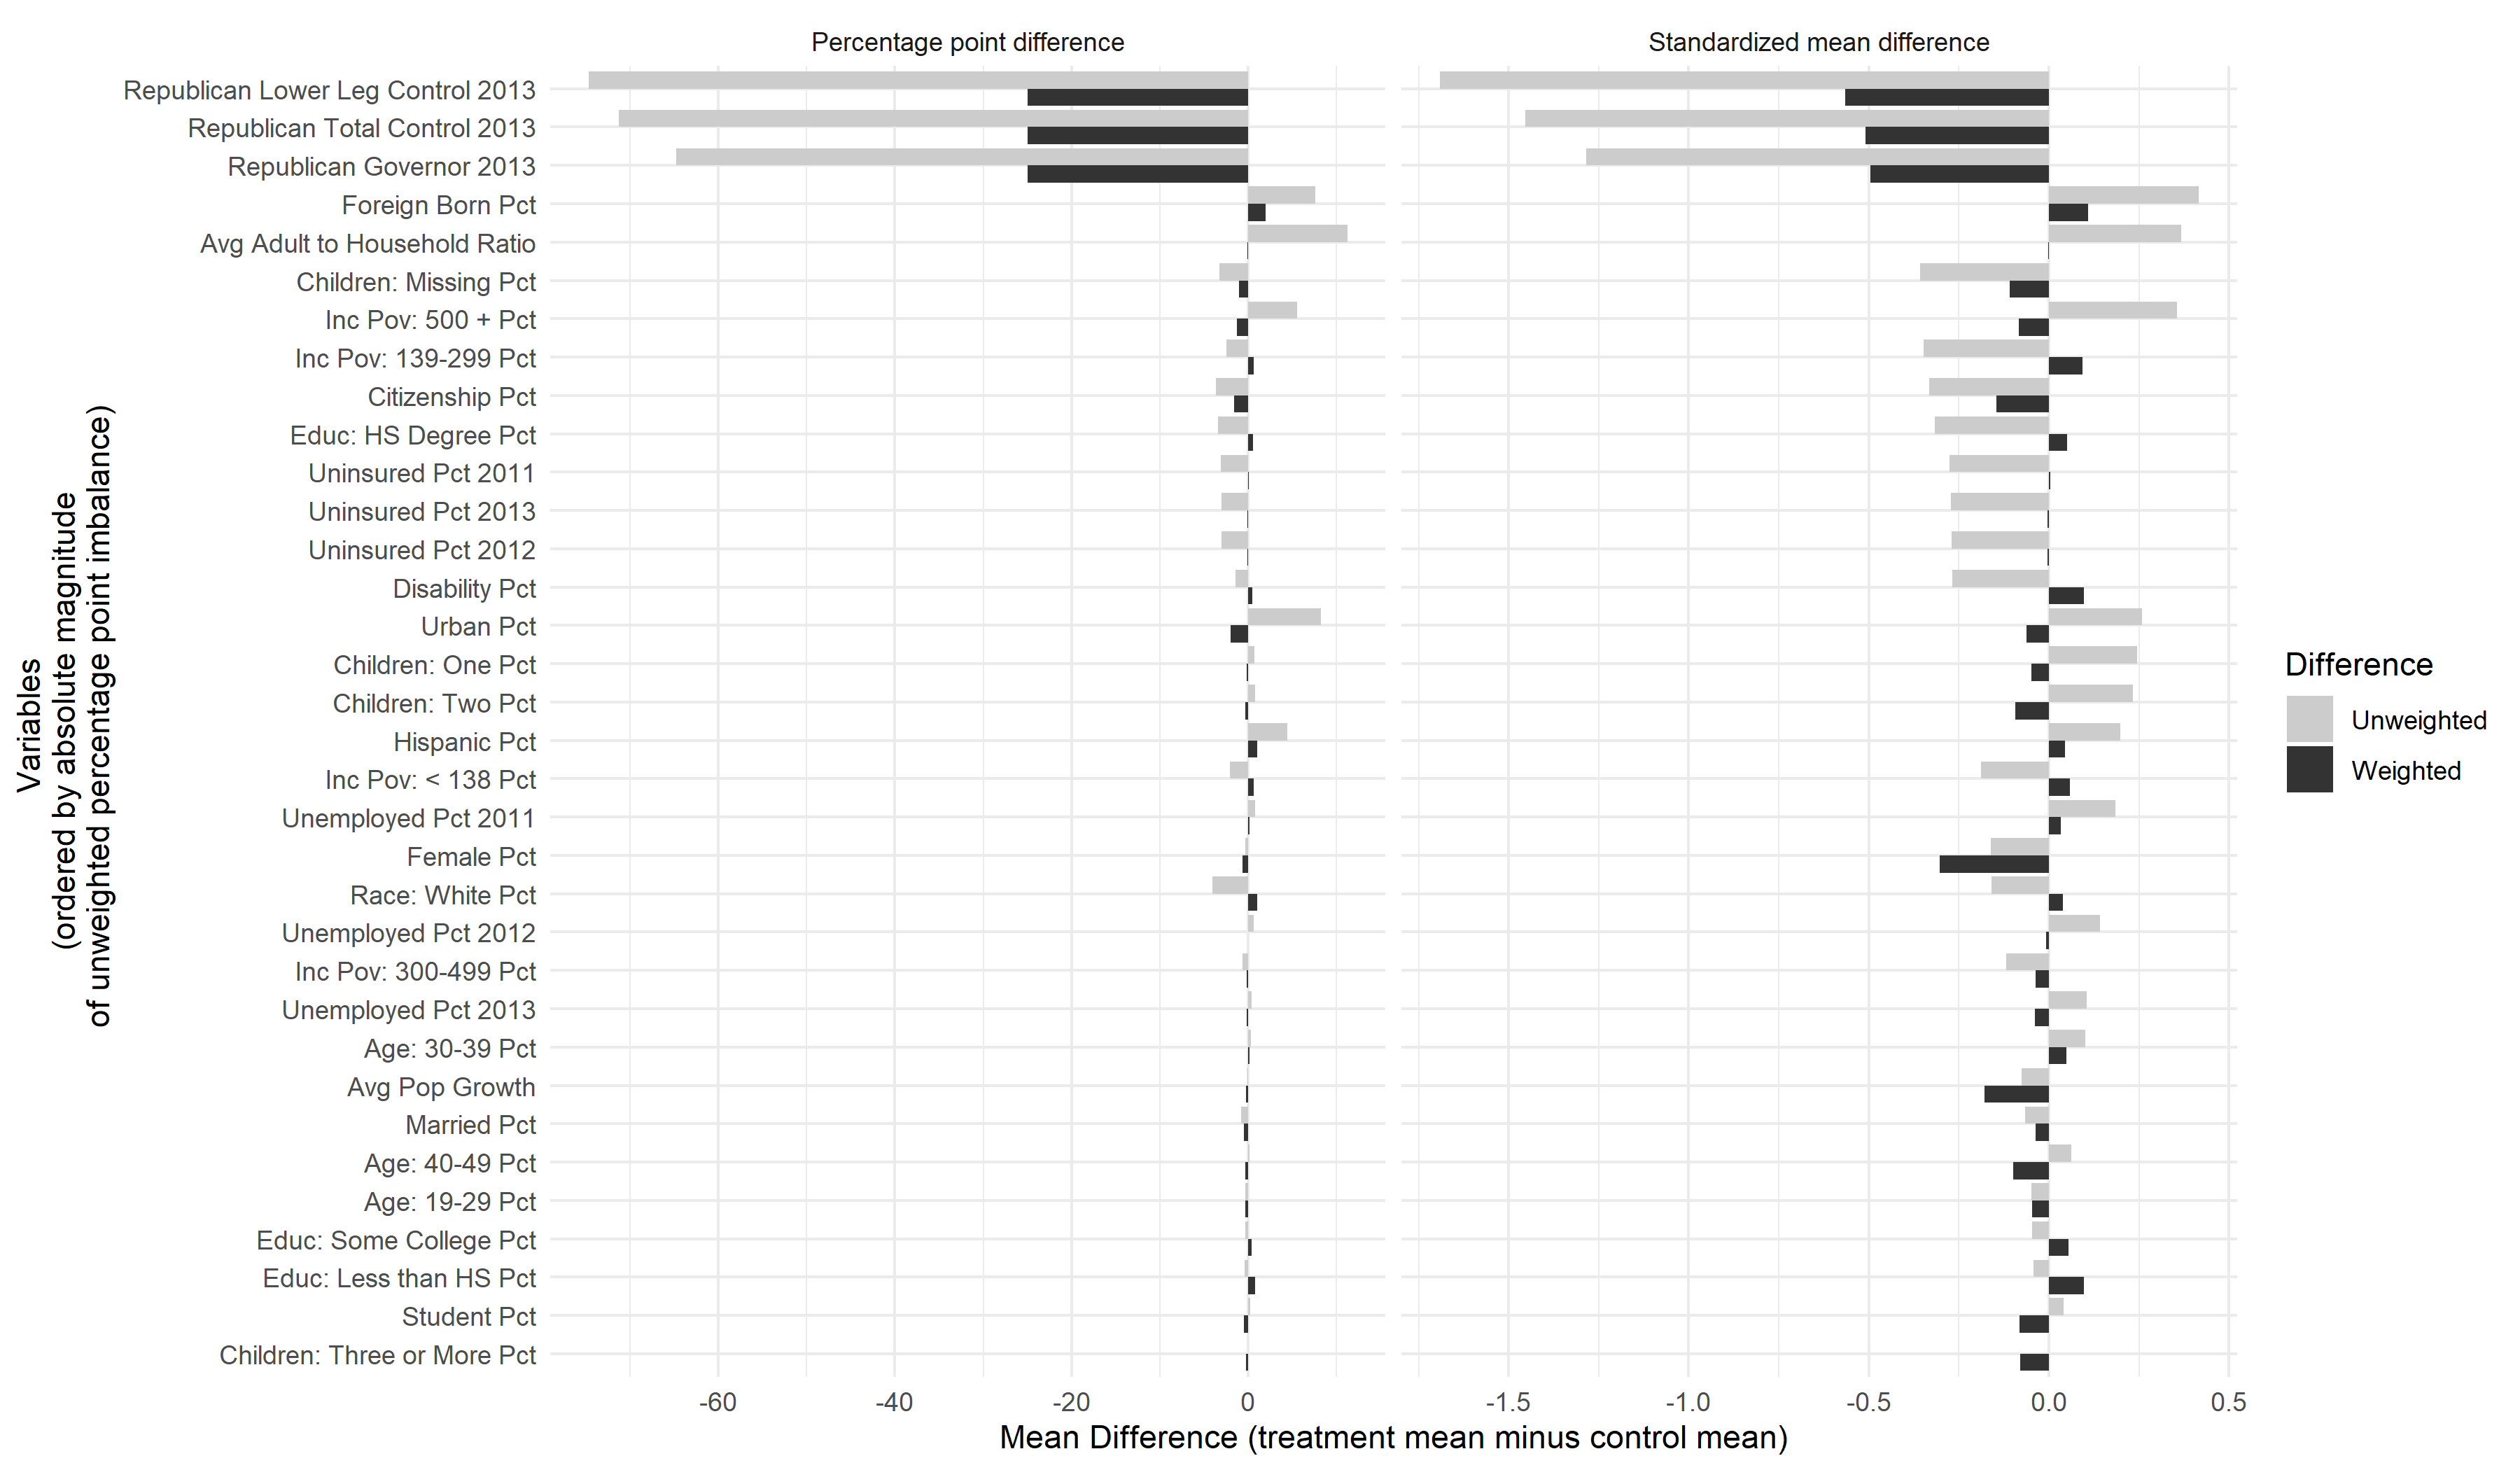
\includegraphics[scale=0.45]{01_Plots/balance-plot-all-etuc1.png}
\end{center}
\end{figure}

\begin{figure}[H]
\begin{center}
    \caption{H-SBW versus BC-HSBW versus SBW, weights summed by state, primary dataset}
    \label{fig:sbwvhsbw1}
    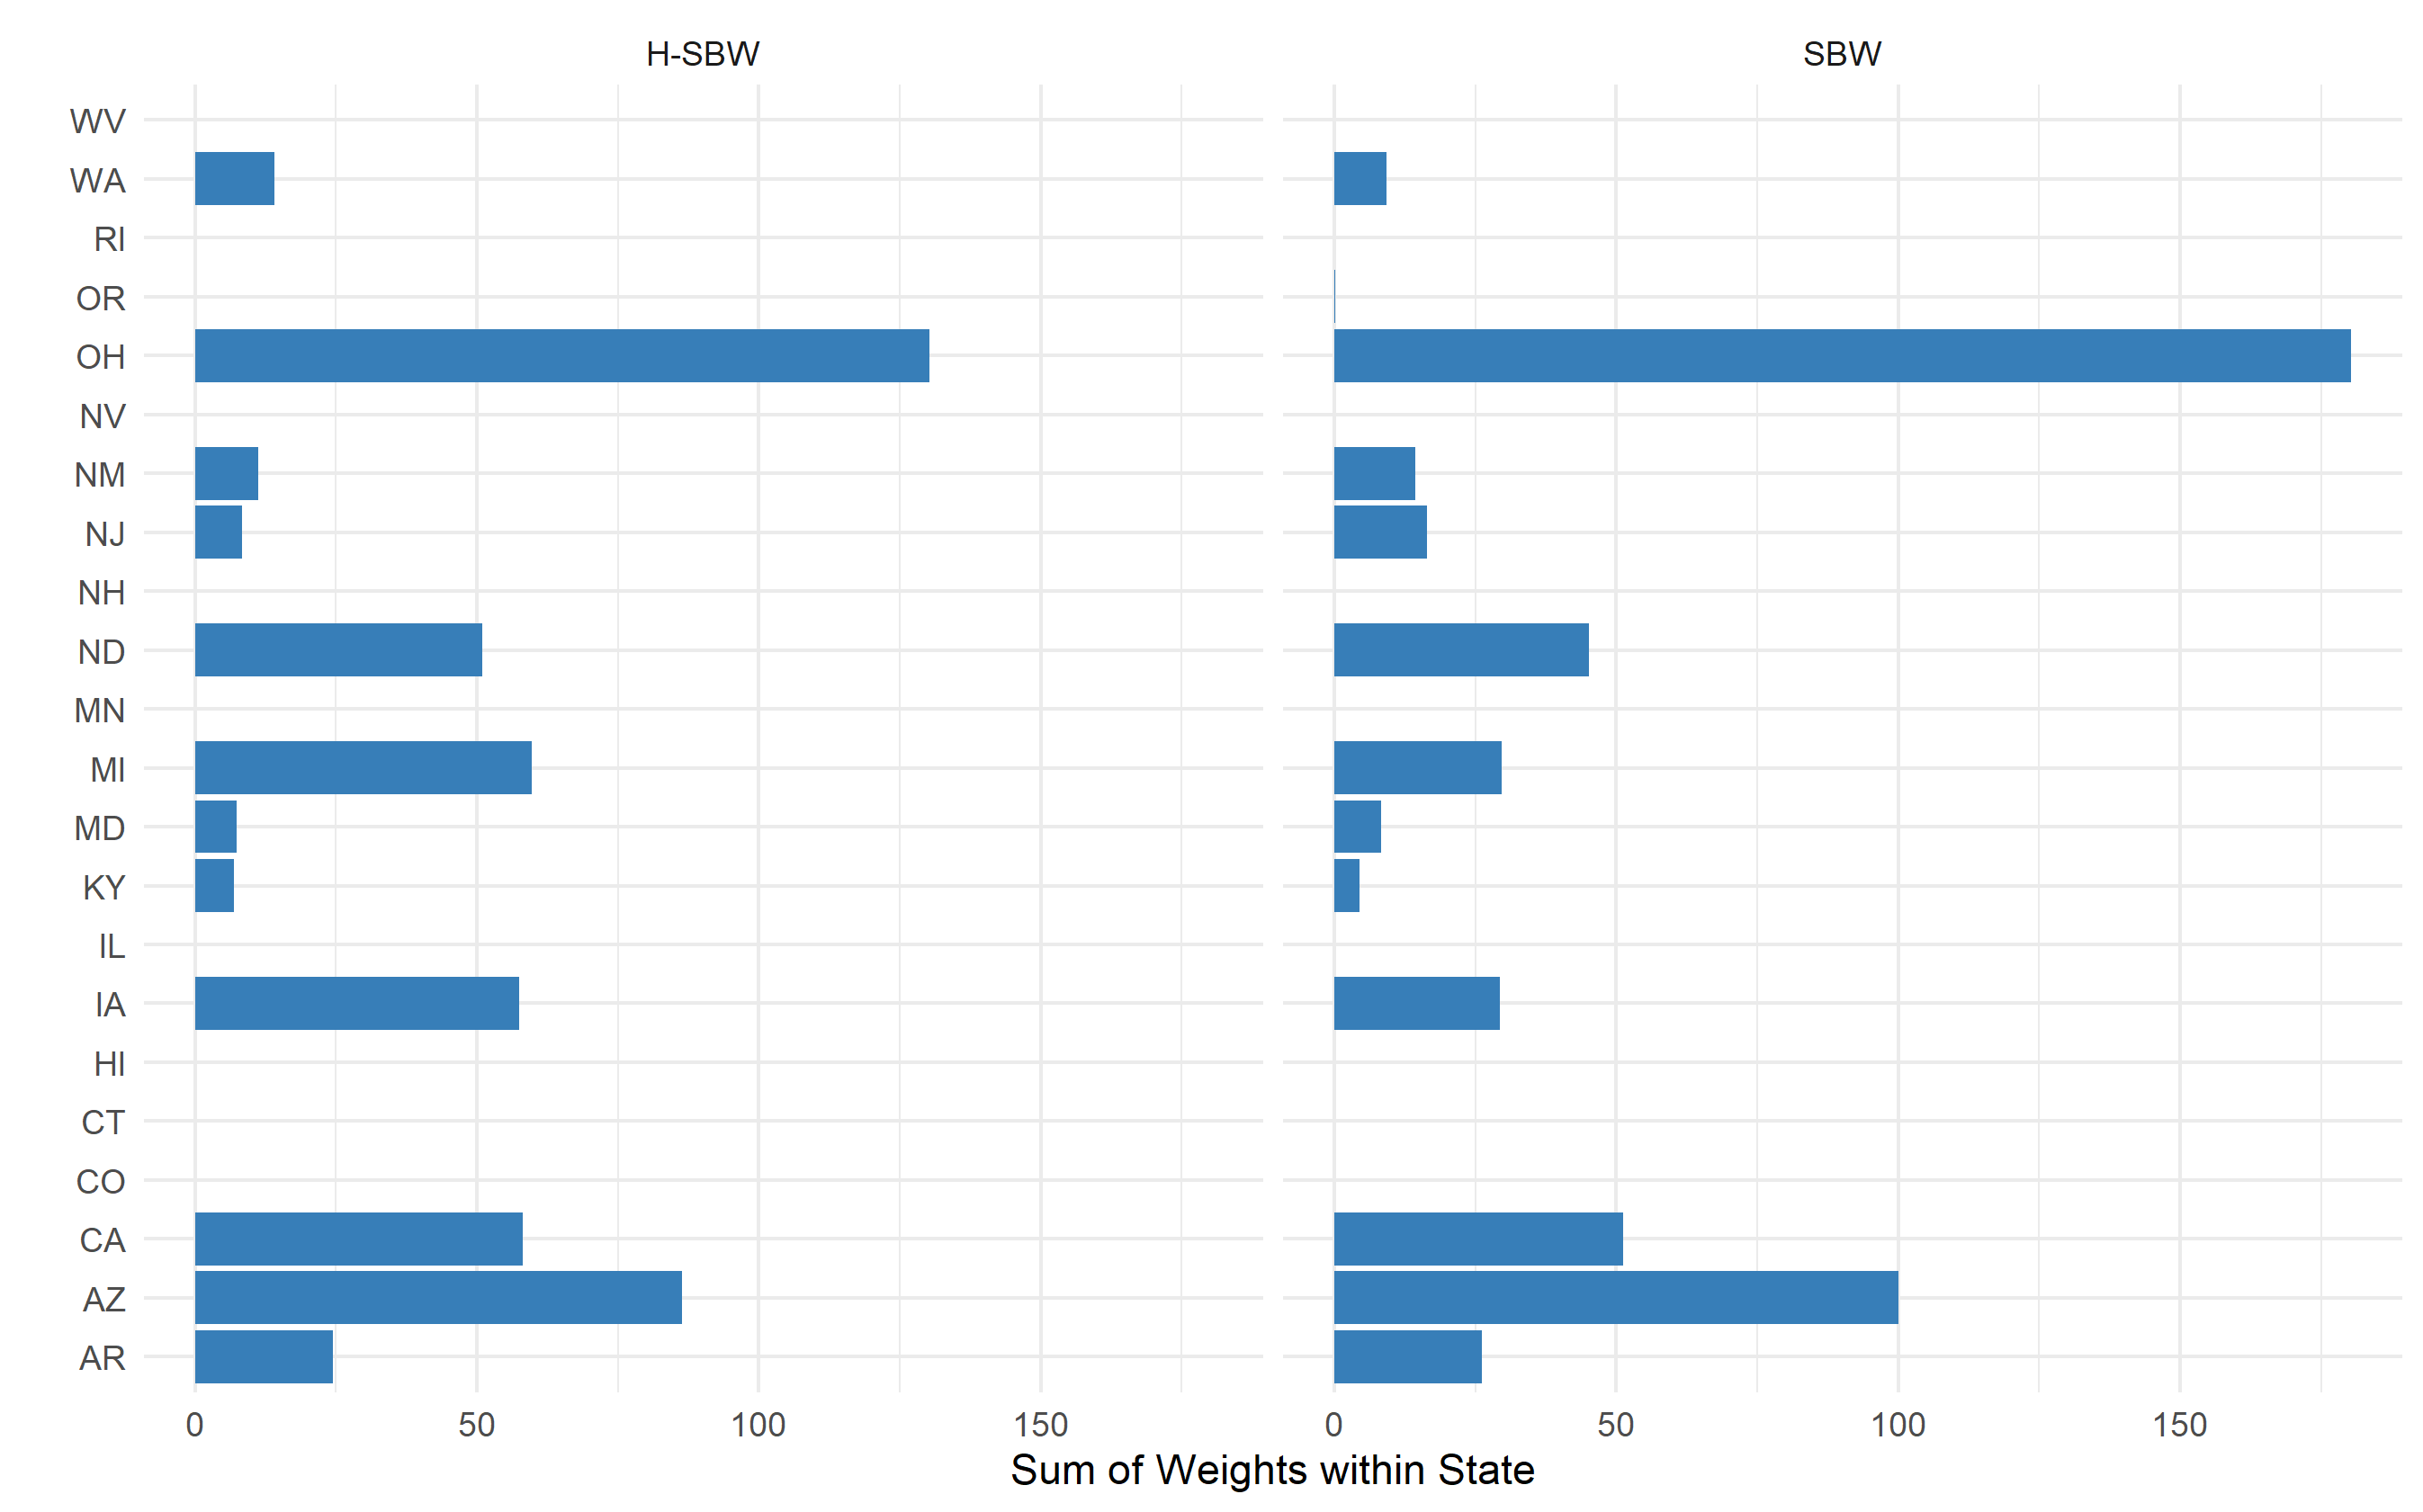
\includegraphics[scale=0.55]{01_Plots/weights-by-state-sbw-hsbw-c1.png}
\end{center}
\end{figure}

To further reduce these imbalances, we also augment these weights using ridge-regression. Figure~\ref{fig:sbwvhsbw1} shows the total weights summed across states (and standardized to sum to 100) for three estimators: H-SBW, BC-HSBW, and SBW. For BC-HSBW we also display the sum the negative weights from the positive weights to highlight the extrapolation. This figure illustrates two key points: first, that H-SBW more evenly disperses the weights across states relative to SBW; second, that BC-HSBW extrapolates somewhat heavily in order to achieve balance, particularly from CPUMAs in California. This is likely in part because California has the most CPUMAs of any state in the dataset.

\subsection{Model validation}\label{sec:validation}

We compare the performance of our models by repeating the covariate adjustments and calculating our procedure on 2009-2011 ACS data to predict 2012 outcomes, and similarly for 2010-2012 data to predict 2013 outcomes for the non-expansion states. We run this procedure using the primary dataset and excluding the early expansion states. Table~\ref{tab:pretxpred} displays the RMSE of these results, with the rows ordered by RMSE for each dataset. We see that the estimators trained on the covariate adjusted data perform substantially better than the unadjusted data and the estimators trained on the homogeneous adjustment outperform their counterparts on the heterogeneous adjustment. We therefore prioritize the results using the homogeneous adjustment. We also observe that H-SBW has comparable performance to SBW throughout.

Interestingly the bias-corrected estimators perform relatively poorly on the primary dataset, but are the best performing estimators when excluding early expansion states -- with RMSEs lower than any other estimator on the primary dataset. As the early expansion states include California, and Figure~\ref{fig:sbwvhsbw1} shows that the bias-corrected estimators extrapolate heavily from this state, the differences in these results suggest that preventing this extrapolation may improve the model's performance. While these results do not imply that the bias-corrected models will perform poorly when predicting $\psi^1_0$ in the post-treatment period on the primary dataset (or that they will perform especially well when excluding the early expansion states), it does highlight the dangers of extrapolation: linearity may approximately hold on the support of the data where we have sufficient covariate overlap, but beyond this region this may be a more costly assumption.\footnote{In Table~\ref{tab:pretxpredfull} in Appendix~\ref{app:allresults}, we also compare the performance against the implied regression weights from OLS and GLS. These weights exactly balance the observed covariates, but are almost always the worst performing estimators in the validation study on either dataset. This also illustrates the benefits of the regularization inherent in the bias-corrected weights.}

\begin{table}[]
    \centering
\begin{longtable}{llrllr}\caption{Estimator pre-treatment outcome RMSE (in \% pts)}\label{tab:pretxpred}
\hline
\multicolumn{3}{c}{Primary data} & \multicolumn{3}{c}{Early expansion 
 excluded} \\ 
%\cmidrule{1-3} \cmidrule{4-6}
\hline
Sigma estimate & Estimator & RMSE & Sigma estimate & Estimator & RMSE \\ 
\hline
Homogeneous & SBW & 0.20 & Homogeneous & BC-HSBW & 0.07 \\ 
Homogeneous & H-SBW & 0.23 & Homogeneous & BC-SBW & 0.12 \\ 
Heterogeneous & SBW & 0.27 & Heterogeneous & BC-HSBW & 0.14 \\ 
Heterogeneous & H-SBW & 0.36 & Heterogeneous & BC-SBW & 0.15 \\ 
Homogeneous & BC-SBW & 0.39 & Homogeneous & H-SBW & 0.25 \\ 
Heterogeneous & BC-SBW & 0.42 & Homogeneous & SBW & 0.26 \\ 
Unadjusted & SBW & 0.56 & Heterogeneous & SBW & 0.28 \\ 
Unadjusted & H-SBW & 0.57 & Heterogeneous & H-SBW & 0.29 \\ 
Homogeneous & BC-HSBW & 0.58 & Unadjusted & SBW & 0.42 \\ 
Heterogeneous & BC-HSBW & 0.63 & Unadjusted & H-SBW & 0.46 \\ 
Unadjusted & BC-SBW & 0.88 & Unadjusted & BC-HSBW & 0.60 \\ 
Unadjusted & BC-HSBW & 0.96 & Unadjusted & BC-SBW & 0.71 \\ 
 \hline
\end{longtable}
\end{table}


Finally, we observe that all estimators generated on the unadjusted dataset under-predict the true uninsurance rate. This may reflect a form of regression-to-the-mean caused by overfitting our weights to noisy covariate measurements. More formally, we can think of the uninsurance rates in time period $t$ in expansion and non-expansion regions as being drawn from separate distributions with means $(\upsilon_1, \upsilon_0)$, respectively, where $\upsilon_1 < \upsilon_0$. For simplicity assume that the only covariate in the outcome model at time $t$ is $Y_{sct-1}$. Under \eqref{eqn:linmod}, we obtain $Y_{sc} = Y_{sct} = \alpha_1 + \beta_1Y_{sct-1} + \epsilon_{sct} + \varepsilon_{st}$. The pre-treatment outcomes are likely positively correlated with the post-treatment outcomes, implying that $\beta_1 > 0$. Because $\upsilon_1 < \upsilon_0$, when reweighting the vector of noisy pre-treatment outcomes $J_{A=1}$ to $\upsilon_0$ the expected value of the weighted measurement error $\mathbb{E}[\sum_{A_{sc} = 1}\hat{\gamma}_{sc}\nu_{sct-1}]$ should be positive. In other words, our weights are likely to favor units with covariate measurements that are greater than their true covariate values. The expected value of the weighted pre-treament outcome will then be less than the target $\upsilon_0$. This implies that our estimates will be negatively biased, since $\mathbb{E}[\beta_1(\sum_{A_{sc} = 1}\hat{\gamma}_{sc}Y_{sct-1} - \upsilon_0)] \le 0$.\footnote{This phenomenon has also been discussed in the difference-in-differences and synthetic controls literature (see, e.g., \cite{daw2018matching}).} While our covariate adjustments are meant to eliminate this bias, in practice they appear more likely only to reduce it. Assuming these errors reflect a (slight) negative bias that will also hold for our estimates of $\psi^1_0$, we may expect that the true treatment effect is closer to zero than our estimates. 

\subsection{Primary Results}

Table~\ref{tab:mainresults} presents all of our estimates. Using H-SBW we estimate an effect of -2.33 (-3.54, -1.11) percentage points on our primary dataset. The SBW results are almost identical with -2.35 (-3.76, -0.95) percentage points. Compared to the unadjusted data we find very similar point estimates at -2.34 (-2.88, -1.79) percentage points for H-SBW and -2.39 (-2.99, -1.79) percentage points for SBW. We see that H-SBW reduces the confidence interval length relative to SBW on our primary dataset, though the lengths are nearly identical when excluding early expansion states. This suggests that H-SBW had at best only modest variance improvements relative to SBW in this setting. Using the adjusted covariate set also increases the length of the confidence intervals relative to the unadjusted data. This increase in the variance estimated is expected in part because the adjustment procedure generally reduces the variability in the data, as we saw in Table~\ref{tab:adjust1}, requiring that the variance of the weights to increase to achieve approximate balance. More generally this increase also reflects the uncertainty due to the measurement error.

Adding the bias-correction decreases the absolute magnitude of the estimates: we estimate effects of -2.05 (-3.30, -0.80) percentage points for BC-HSBW and -2.07 (-3.14, -1.00) percentage points for BC-SBW. This contrasts to our validation tests, where the bias-corrected estimators tended to predict lower uninsurance rates than the other estimators. The point estimates from the SBW and H-SBW estimators were virtually identical. The estimates calculated using the heterogeneous adjustment were all closer to zero than the unadjusted estimates (results are available in Appendix~\ref{app:allresults}).

\begin{table}[ht]
\begin{longtable}{lllrlr}\caption{Primary results}\label{tab:mainresults} \\
 \hline
 &  & \multicolumn{2}{c}{Primary data} & \multicolumn{2}{c}{Early expansion 
 excluded} \\
  \hline
Weights & Adjustment & Estimate  & Difference & Estimate & Difference\\ 
 &  & (95\% CI) &  & (95\% CI) & \\
  \hline
H-SBW & Homogeneous & -2.33 (-3.54, -1.11) & 0.01 & -2.09 (-3.24, -0.94) & 0.19 \\ 
  H-SBW & Unadjusted & -2.34 (-2.88, -1.79) & - & -2.28 (-2.87, -1.70) & - \\ 
  BC-HSBW & Homogeneous & -2.05 (-3.30, -0.80) & 0.17 & -1.94 (-3.27, -0.61) & 0.28 \\ 
  BC-HSBW & Unadjusted & -2.22 (-2.91, -1.52) & - & -2.22 (-3.14, -1.31) & - \\ 
  SBW & Homogeneous & -2.35 (-3.76, -0.95) & 0.04 & -2.05 (-3.19, -0.91) & 0.16 \\ 
  SBW & Unadjusted & -2.39 (-2.99, -1.79) & - & -2.21 (-2.75, -1.68) & - \\ 
  BC-SBW & Homogeneous & -2.07 (-3.14, -1.00) & 0.13 & -1.99 (-3.33, -0.66) & 0.23 \\ 
  BC-SBW & Unadjusted & -2.19 (-2.94, -1.45) & - & -2.23 (-3.12, -1.33) & - \\    
  \hline
\end{longtable}
\subcaption{``Difference'' column reflects difference between adjusted and unadjusted estimators}
\end{table}

All adjusted estimators were closer to zero than the corresponding unadjusted estimators. However, the difference between the adjusted SBW and H-SBW and the unadjusted versions is close to zero. This is in contrast to our validation study where the unadjusted SBW and H-SBW estimators ranged from about 0.3 to 0.4 percentage points lower than the adjusted estimators.\footnote{When excluding the early expansion states, the difference between the estimates on the adjusted and unadjusted data persist but are also smaller in magnitude.} We interpret this difference as due to chance: while theory and our validation study suggests that our unadjusted estimators are biased, bias only exists in expectation. Our primary dataset is a random draw where our unadjusted estimators perform more comparably to the adjusted estimators.

We next consider the sensitivity of our analysis with respect to the no anticipatory treatment effects assumption by excluding the early expansion states (California, Connecticut, Minnesota, New Jersey, and Washington) and re-running our analyses. The column ``Early excluded estimate (95\% CI)'' in Table~\ref{tab:mainresults} reflects these results. The overall patterns of the results are consistent with our primary estimates; however, our point estimates almost all move somewhat closer to zero. This may indicate that either the primary estimators have a slight negative bias, or that these estimates have a slight positive bias. Given our analysis of the validation study we view the first case as more likely. This would imply that our primary estimators reflect a lower bound on the true treatment effect. Regardless, the differences are small relative to our uncertainty estimates. Overall we view our primary results as relatively robust to the exclusion of these states. Additional diagnostics and results are available in Appendix~\ref{app:weightdiagnostics}.

\section{Discussion}

We divide our discussion into two sections: methodological considerations and policy considerations. 

\subsection{Methodological considerations and limitations}

We make multiple contributions to the literature on balancing weights. First, our estimation procedure accounts for mean-zero random noise in our covariates that is uncorrelated with the outcome errors. We modify the SBW constraint set to balance on a linear approximation to the true covariate values, applying the idea of regression calibration from the measurement error literature to the context of balancing weights. Our results illustrate the benefits of this procedure: using observed pre-treatment outcomes generated by an unknown data generating mechanism, Table~\ref{tab:pretxpred} demonstrates that our proposed estimators have better predictive performance when balancing on the adjusted covariates. This finding is consistent with concerns about overfitting to noisy covariate measurements and subsequent regression-to-the-mean.

This approach has several limitations: first, it requires access to auxiliary data with which to estimate the measurement error covariance matrix $\Sigma_{\nu}$. Many applications may not have access to such information. Even without such data, $\Sigma_{\nu}$ could also be considered a sensitivity parameter to evaluate the robustness of results to measurement error (see, e.g., \cite{huque2014impact}, \cite{illenberger2020impact}). Second, from a theoretic perspective, we require strong distributional assumptions on the covariates to consistently estimate $\psi_0^1$ using convex balancing weights. This contrasts to \cite{gleser1992importance}, who shows that the OLS estimates are consistent with only very weak distributional assumptions on the data (see also Propositions~\ref{cl8} and ~\ref{cl9} in Appendix~\ref{app:AsecI}). This relates to a third limitation: we require strong outcome modeling assumptions. Yet by preventing extrapolation, SBW and H-SBW estimates may be less sensitive than OLS estimates to these assumptions. Our validation results support this: the standard regression calibration adjustment using OLS and GLS weights performs the worst out of any methods we consider (see Table~\ref{tab:pretxpredfull} in Appendix~\ref{app:allresults}). In contrast, using regression-calibration with balancing weights -- even when allowing for limited extrapolation using ridge-augmentation -- performs better.\footnote{We also provide a suggestion of how to adapt our procedure to accommodate a basis expansion of gaussian covariates in Appendix~\ref{app:AsecI} Remark~\ref{remark:basis expansion}}. Developing methods to relax these assumptions further would be a valuable area for future work.

A final concern is that this procedure may be sub-optimal with respect to the mean-square error of our estimator. In particular, the bias induced by the measurement error decreases with the sample size used to calculate each CPUMA's covariate values, the minimum of which were over three hundred. Yet the variance of our counterfactual estimate decreases with the number of treated states. From a theoretic perspective, the variance is of a larger order than the bias, so perhaps the bias from measurement error should not be a first-order concern. Our final results support this: the changes in our results on the adjusted versus unadjusted data are of smaller magnitude than the associated uncertainty estimates. Other studies have proposed tests of whether the measurement error corrections are ``worth it'', though we do not do this here (see, e.g., \cite{gleser1992importance}). However, as an informal observation, our simulation study in Appendix~\ref{app:simstudy} shows that the MSE of the SBW estimator that naively balances on the noisy covariates $W$ is comparable to the MSE of the SBW estimator that balances on the adjusted covariates $\hat{X}$ when the ratio of the variance of $X$ to the variance of $W$ is over 0.95. However, even in this setting we find that confidence interval coverage can fall below nominal rates when balancing on $W$, and that the measurement error correction can improve our ability to construct valid confidence intervals.

Our second contribution is to introduce the H-SBW objective. This objective can improve upon the SBW objective assuming that the errors in the outcome model are homoskedastic with constant positive equicorrelation $\rho$ within known groups of units. Assuming no measurement error and that $\rho$ is known, we show that H-SBW returns the minimum variance estimator within the constraint set by more evenly dispersing weights across the groups. We also demonstrate the connection between these weights and the implied weights from GLS (see Propositions~\ref{cl4} and \ref{cl56} in Appendix~\ref{app:AsecII}). While studies have considered balancing weights in settings with hierarchical data (see, e.g., \cite{keele2020hospital}), we are the first to our knowledge to propose changing the criterion to account for correlated outcomes.

This estimation procedure has at least three potential drawbacks. First, we make a very specific assumption on the covariance structure of the error terms that is useful for our application. Applications where a different structure $\Omega$ is more appropriate one can still follow our approach and minimize the more general criterion $f(\gamma) = \gamma^T\Omega\gamma$. Second, we require specifying the parameters $(\rho, \delta)$ in advance. Choosing $\delta$ is a challenging problem shared with SBW and we do not offer any new suggestions.\footnote{We refer to \cite{wang2020minimal} who offer an interesting data-driven approach to this problem.} Choosing $\rho$ is a new problem of this estimation procedure. Encouragingly, our simulation study shows the H-SBW estimator for any chosen $\rho$ almost always has lower variance than SBW in the presence of state-level random effects (see Appendix~\ref{app:simstudy}).\footnote{We caution that this finding solely reflects the simulation space we examined.} Even so, identifying a principled approach to choosing this parameter would be a useful future contribution. Third, in the presence of both measurement error and dependent data, using H-SBW in combination with the standard regression-calibration adjustment may be biased. This bias arises because the standard adjustment assumes independent observations. Our simulations show that this bias can increase with $\rho$ and that SBW remains approximately unbiased if the covariates are gaussian - though H-SBW may still have modest MSE improvements. We also show a theoretical modification to the adjustment procedure so that H-SBW will return unbiased estimates in this setting (see Propositions~\ref{cl7} and ~\ref{cl7hsbw}).

\subsection{Policy considerations and limitations}

We estimate that had states that did not expand Medicaid in 2014 instead expanded their programs, they would have seen a -2.33 (-3.54, -1.11) percentage point change in the average adult uninsurance rate. Our validation study and robustness checks indicate that this estimate may be biased downwards (away from zero), in which case we can interpret this estimate as a lower bound on the ETC. Existing estimates place the ETT between -3 and -6 percentage points. These estimates vary depending on the targeted sub-population of interest, the data used, the level of modeling (individuals or regions), and the modeling approach (see, e.g., \cite{courtemanche2017early}, \cite{kaestner2017effects}, \cite{frean2017premium}). Our estimate of the ETC are closer to zero than these estimates. When we attempt to estimate the ETT using our proposed method, the resulting estimates have high uncertainty due to limited covariate overlap.\footnote{In particular, there were no states entirely controlled by Democrats that did not expand Medicaid. Even allowing for large imbalances, our standard error estimates were approximately three percentage points and our confidence intervals all contained zero. When estimating a simple difference-in-differences model on the unadjusted dataset we estimate that the ETT is -2.05 (-3.23, -0.87), where the standard errors account for clustering at the state level.\label{footnote_did}} The differences may reflect different modeling strategies and data, or it may suggest that the ETC is smaller in absolute magnitude than the ETT.

We ultimately make no formal statistical claims about these differences, but we do emphasize the importance of caution when using estimates of the ETT to make inferences about the ETC. Because almost every outcome of interest is mediated through increasing the number of insured individuals, if the ETC is in fact different than the ETT, then projecting findings from an estimate of the ETT to the ETC may lead to inaccurate inferences. For example, \cite{miller2019medicaid} study the effect of Medicaid expansion on mortality. Using their estimate of the ETT they project that had all states expanded Medicaid, 15,600 deaths would have been avoided during their study's time-period. If we believe that this number increases monotonically with the number of uninsured individuals, this estimate may be an overestimate if the ETC is less than the ETT, or an underestimate if the ETC is greater than the ETT. Directly estimating the ETC can help us better model policy relevant downstream effects mediated through changing the uninsurance rate. 

Our estimate is not without limitations. Specifically, our analysis requires many strong modeling assumptions. In particular, we require SUTVA, no anticipatory treatment effects, no unmeasured confounding conditional on the true covariates, and several parametric assumptions regarding the outcome and measurement error models. We have addressed some concerns about possible violations of these assumptions. For example, our results were qualitatively similar whether we excluded possible ``early expansion states,'' or used different weighting strategies (including relaxing the positivity restrictions and changing the tuning parameter $\rho$). However, we do not attempt to address concerns about the impact of spillovers across regions. And while we believe that no unmeasured confounding is reasonable for this problem, we did not conduct a sensitivity analysis (see, e.g., \cite{bonvini2021sensitivity}) with respect to this assumption. 

Medicaid expansion remains an ongoing policy debate in the United States, with states such as Wyoming, Alabama, and North Carolina reportedly considering expanding their programs. Our study estimates the effect of Medicaid expansion on adult uninsurance rates; however, the primary reason this effect interesting is that Medicaid enrollment is not automatic for eligible individuals. If the goal of Medicaid expansion is to increase insurance access for low-income adults, state policy-makers also may wish to make it easier or even automatic to enroll in Medicaid. 

\section{Conclusion}

We predict the average change in the non-elderly adult uninsurance rate in 2014 among states that did not expand their Medicaid eligibility thresholds as if they had. We use survey data aggregated to the CPUMA-level to estimate this quantity. The resulting dataset has both measurement error in the covariates that may bias standard estimation approaches, and a hierarchical structure that may increase the variance of these same approaches. We therefore propose an estimation procedure that uses balancing weights that accounts for these problems. We demonstrate that our bias-reduction approach improves on existing methods when predicting observed outcomes from an unknown data generating mechanism. Applying this method to our problem, we estimate that states that did not expand Medicaid in 2014 would have seen a -2.33 (-3.54, -1.11) percentage point change in their adult uninsurance rates had they done so. This is the first study we are aware of that directly estimates the treatment effect on the controls with respect to Medicaid expansion. From a methodological perspective, we demonstrate the value of our proposed method relative to existing methods. From a policy-analysis perspective, we emphasize the importance of directly estimating the relevant causal quantity of interest. More generally if the goal of Medicaid expansion is to improve access to insurance, state and federal policy-makers should consider policies that make Medicaid enrollment easier if not automatic.

\section*{Acknowledgements}

The authors gratefully acknowledge invaluable advice and comments from Zachary Branson, Riccardo Fogliato, Edward Kennedy, Brian Kovak, Akshaya Jha, Lowell Taylor, and Jose Zubizaretta.

\begin{supplement}
Analyses conducted using R Version 4.0.2 (\cite{r}), and the optweight (\cite{optweight}) and tidyverse (\cite{tidyverse}) packages. Programs and supporting materials are available at \url{github.com /mrubinst757/medicaid-expansion}. Proofs and additional results are available in the Appendix. 
\end{supplement}

\bibliographystyle{imsart-nameyear} % Style BST file
\bibliography{research.bib}       % Bibliography file (usually '*.bib')

\clearpage

\appendix

\section{Proofs}\label{ssec:proof}

We divide our proofs into three sections: the first two consist of propositions and the third contains the proofs of the propositions. In the first section our propositions pertain to the performance of SBW under the classical measurement error model. Our key results are that the bias of the SBW estimator is equivalent to the bias of the OLS estimator and that regression-calibration techniques can be used in this setting to obtain consistent estimators. However, these results assume that the data are gaussian. We also show that if the data are not gaussian, the OLS estimator using regression-calibration remains consistent, while the SBW estimator may be biased. In our second section we consider the properties of the H-SBW objective when the true covariates $X$ are observed. We show that if our assumed correlation structure for the outcome errors is correct, H-SBW produces the minimum conditional-on-X variance estimator within the constraint set. We also show how a generalized form of H-SBW weights relate to the implied regression weights from Generalized Least Squares (GLS). We conclude by showing that H-SBW may yield biased estimates if we do not correctly model the dependence structure of the data. Section~\ref{app:AsecIII} contains all of the proofs.

\subsection{SBW and classical measurement error}\label{app:AsecI}

We begin by showing six results regarding the bias of the OLS and SBW estimators under the classical errors-in-variables model. First, we show that without adjustment for errors-in-covariates, the bias of the SBW estimator that sets $\delta = 0$ (i.e. reweights the treated units to exactly balance the control units) is equal to the bias of the OLS estimator. Second, we show that if the observed covariate values for the treated data can be replaced by their conditional expectations $\tilde{X}$ given the noisy observations, then the SBW estimator will be unbiased and consistent. Third, we consider the case where $\tilde{X}$ must be estimated, and show that the SBW estimator is consistent if we replace $\tilde{X}$ by a consistent estimate $\hat{X}$. Finally, we remove the assumption that $X$ is gaussian, and show that while the OLS estimator remains unbiased under weaker assumptions, the SBW estimator does not, and we show a general expression for the asymptotic bias. We take the perspective throughout that $X$ is random among the treated units but fixed for the control units.

We assume that equations (\ref{eqn:unconfoundedness}) - (\ref{eqn:Xgaussian}) hold. For simplicity, we additionally assume that
\begin{equation}\label{eqn:simplifications}
\epsilon_{sc} = 0, \quad \varepsilon_s = 0,\quad \xi_{sc} = 0,\quad  \Sigma_{\nu,sc} = \Sigma_\nu, \qquad \forall s,c
\end{equation}
noting that $\xi_{sc}=0$ implies $J_{sc} = Y_{sc}$. The covariate observations of the treated units can then be seen to be i.i.d., with covariance matrix
\[ \Sigma_{W|1} = \Sigma_{X|1} + \Sigma_\nu,\]
and the conditional expectation of $X_{sc}$ given $W_{sc}$ for the treated units can be seen to equal
\[ \tilde{X}_{sc} = v_1 + \kappa^T (W_{sc} - v_1), \qquad \forall sc: A_{sc}=1,\]
where
\[ \kappa = (\Sigma_{X|1} + \Sigma_{\nu})^{-1} \Sigma_{X|1}.\]
To ease notation, we abbreviate $\Sigma_X = \Sigma_{X \mid 1}$ and similarly $ \Sigma_W = \Sigma_{W \mid 1}$. 

In Propositions \ref{cl8}, \ref{cl9}, and part of Proposition \ref{cl1}, we will remove the Gaussian covariate assumption given by \eqref{eqn:Xgaussian}. In its place, we will instead consider the weaker assumption that the empirical covariance of $X$ has a limit $S_X$,

\begin{equation}\label{eqn:limitX}
 \frac{1}{n_1} \sum_{A_{sc}=1} (X_{sc} - \bar{X}_1)(X_{sc} - \bar{X}_1)^T \rightarrow^p S_X,
\end{equation}
which implies a similar limit $S_W$ for the noisy observations $W$,

\begin{equation}\label{eqn:limitW}
 \frac{1}{n_1} \sum_{A_{sc}=1} (W_{sc} - \bar{W}_1)(W_{sc} - \bar{W}_1)^T \rightarrow^p S_W = S_X + \Sigma_{\nu},
\end{equation}
where we have used the independence of the noise terms $\nu_{sc}$, and similarly that 
\begin{equation}\label{eqn:limitWY}
 \frac{1}{n_1} \sum_{A_{sc}=1} (W_{sc} - \bar{W}_1)(Y_{sc} - \bar{Y}_1)^T \rightarrow^p S_X \beta_1,
\end{equation}
where we have additionally used the linear model for $Y_{sc}$ given by \eqref{eqn:linmod}.

We first consider estimation without adjustment for errors in covariates. 
Proposition \ref{cl1} states that the unadjusted OLS and SBW estimators have equal bias, with the bias of the OLS estimator remaining unchanged if the gaussian assumption of \eqref{eqn:gaussiannoise} is removed.

\begin{proposition}\label{cl1}
Let (\ref{eqn:unconfoundedness}) - (\ref{eqn:Xgaussian}) and (\ref{eqn:simplifications}) hold.
Let $(\hat{\alpha}, \hat{\beta})$ denote the unadjusted OLS estimator of $(\alpha_1, \beta_1)$, 
\begin{equation}\label{eqn:prop1.beta}
(\hat{\alpha}, \hat{\beta}) = \arg \min_{\alpha, \beta} \sum_{sc:A_{sc}=1} (Y_{sc} - \alpha -  W_{sc}^T\beta)^2,
\end{equation}
which induces the OLS estimator of $\psi_0^1$ given by

\begin{align*}
\hat{\psi}^{1,\textup{ols}}_0 = \bar{Y}_1 + (\bar{W}_0 - \bar{W}_1)^T\hat{\beta}_1.
\end{align*}
%
Let ${\gamma}$ denote the unadjusted SBW weights under exact balance, found by solving \eqref{eqn:SBWobjective} with constraint set $\Gamma( W_{A=1}, \bar{W}_0, 0)$, which induces the SBW estimator of $\psi_0^1$ given by

\begin{align*}
\hat{\psi}^{1,\textup{sbw}}_0 = \sum_{sc: A_{sc} = 1} {\gamma}_{sc} Y_{sc}.
\end{align*}
%
Then the estimators $\hat{\psi}^{1, \textup{ols}}_0$ and $\hat{\psi}^{1, \textup{sbw}}_0$ have equal bias, satisfying

\begin{align*}
\mathbb{E}[\hat{\psi}_0^{1,\textup{ols}}] &= \mathbb{E}[\hat{\psi}^{1, \textup{sbw}}_0]  = \psi_0^1 + (\bar{X}_0 - \upsilon_1)^T(\mathbf{\kappa} - I_q)\beta.
\end{align*}
Additionally, the bias of $\hat{\psi}_0^{1,\textup{ols}}$ is asymptotically unchanged if the gaussian covariate assumption given by \eqref{eqn:Xgaussian} is replaced by \eqref{eqn:limitX}.
\end{proposition}

To study the SBW estimator with covariate adjustment, we first consider an idealized version where $\Sigma_X$ and $\Sigma_\nu$ are known, so that $\tilde{X}_{A=1}$ is also known. Proposition \ref{cl2} shows that the resulting estimate of $\psi_0^1$ is unbiased if $\delta = 0$.

\begin{proposition}\label{cl2}
Let (\ref{eqn:unconfoundedness}) - (\ref{eqn:Xgaussian}) and (\ref{eqn:simplifications}) hold. Let $\tilde{X}_{A=1}$ equal the conditional expectation of $X_{A=1}$ given $W$,

\[ \tilde{X}_{sc} = \upsilon_1 + \kappa^T (W_{sc} - \upsilon_1), \qquad \forall sc: A_{sc} = 1,\] let $\gamma^*$ be the solution to the SBW objective defined over the constraint set $\Gamma(\tilde{X}_{A=1}, \bar{X}_0, 0)$, and let $\hat{\psi}^{1, \textup{ideal}}_0$ be the SBW estimator $\sum_{sc: A_{sc} = 1}\gamma^\star_{sc}Y_{sc}$. This estimator is unbiased for $\psi_0^1$.
\end{proposition}



Proposition \ref{prop:variance_rate} shows that the variance of this idealized SBW estimator goes to zero, implying consistency. 
\begin{proposition}\label{prop:variance_rate}
Let (\ref{eqn:unconfoundedness}) - (\ref{eqn:Xgaussian}) and (\ref{eqn:simplifications}) hold, and let $\gamma^*$ and $\hat{\psi}_0^{1, \textup{ideal}}$ be defined as in Proposition \ref{cl2}. Then the conditional variance of the estimation error is given by

\begin{align*}
\operatorname{Var}\left( \hat{\psi}_0^{1, \textup{ideal}} - \psi_0^1| W\right)  = \|\gamma^*\|^2 \cdot \beta_1^T(\Sigma_{X} - \Sigma_{X}\Sigma_{W}^{-1}\Sigma_{X})\beta_1, 
\end{align*}
with $\operatorname{Var}\left( \hat{\psi}_0^{1, \textup{ideal}} - \psi_0^1| W\right)$ and $\operatorname{Var}(\hat{\psi}_0^{1,\textup{ideal}})$ both behaving as $O_P(n_1^{-1})$ as $n_1 \rightarrow \infty$.
\end{proposition}

In practice, the idealized SBW estimator considered in Propositions \ref{cl2} and \ref{prop:variance_rate} cannot be used, as $\Sigma_X$ and $\Sigma_{\nu}$ are not known, but instead must be estimated from auxilliary data. Proposition \ref{cl3} states that if these estimates are consistent, then the resulting adjusted SBW estimator for $\psi_0^1$ is also consistent if $\delta = 0$.

\begin{proposition}\label{cl3}
Let (\ref{eqn:unconfoundedness}) - (\ref{eqn:Xgaussian}) and (\ref{eqn:simplifications}) hold. Given estimates $\hat{\Sigma}_X$ and $\hat{\Sigma}_\nu$ that are consistent for $\Sigma_X$ and $\Sigma_\nu$, let $\hat{X}_{A=1}$ be given by 
\[ \hat{X}_{sc} = \bar{W}_1 + \hat{\kappa}^T(W_{sc} - \bar{W}_1), \]
where $\hat{\kappa} = (\hat{\Sigma}_X + \hat{\Sigma}_{\nu})^{-1} \hat{\Sigma}_X$. Let $\hat{\gamma}$ be the weights that solve the SBW objective over the constraint set $\Gamma(\hat{X}_{A=1}, \bar{W}_0, 0)$, and let $\hat{\psi}^{1, \textup{adjusted}}_0 = \sum_{sc: A_{sc} = 1} \hat{\gamma}_{sc} Y_{sc}$ be the corresponding SBW estimator. This estimator is consistent for $\psi_0^1$ as $n_1 \to \infty$.
\end{proposition}

In (\ref{eqn:jackknife}) we propose a leave-one-state-out jackknife estimate of variance. Following \cite{efron1981jackknife}, this estimate can be decomposed a conservatively biased estimate of the variance of $\hat{\psi}_0^{1, \textup{adjusted}}$ given a sample size of $(m_1-1)$ treated states, plus a heuristic adjustment to go from sample size $(m_1-1)$ to sample size $m_1$, when treating the observations of the control states as fixed.

\begin{proposition}\label{prop:jackknife}
Let (\ref{eqn:unconfoundedness}) - (\ref{eqn:gaussiannoise}) hold, and additionally assume that $p_s$, the number of CPUMAs, is i.i.d. in the treated states. Let $\hat{\operatorname{Var}}(\hat{\psi}_0^{1, \textup{adjusted}}) = \frac{m_1-1}{m_1} \cdot \tilde{\operatorname{Var}}(\hat{\psi}_0^{1, \textup{adjusted}})$, where

\begin{equation} \label{eqn:prop.jackknife}
\tilde{\operatorname{Var}}(\hat{\psi}_0^{1, \textup{adjusted}}) = \sum_{s:A_{s}=1} (S_{(s)} - S_{(\cdot)})^2,
\end{equation}
with $S_{(s)}$ and $S_{(\cdot)}$ as defined for \eqref{eqn:jackknife}. Then $\tilde{\operatorname{Var}}$ is conservatively biased for the variance of the leave-one-state-out estimate,

\[ \mathbb{E}\left[ \tilde{\operatorname{Var}}(\hat{\psi}_0^{1, \textup{adjusted}})\right] \geq \operatorname{Var}(S_{(1)} | \bar{W}_0),\]
where $S_{(1)}$ can be seen to equal the estimator $\hat{\psi}_0^{1,\textup{adjusted}}$ under a sample size of $(m_1-1)$ treated states.

\end{proposition}

As the gaussian covariate assumption given by \eqref{eqn:Xgaussian} is strong, it would be desirable if the adjusted OLS or SBW estimators were consistent even for non-gaussian $X$. Proposition \ref{cl8} shows under mild assumptions that this is in fact true when running OLS on the adjusted covariates. 

\begin{proposition}\label{cl8}
Let (\ref{eqn:unconfoundedness}) - (\ref{eqn:gaussiannoise}), and (\ref{eqn:simplifications})- (\ref{eqn:limitX}) hold, with $S_X$ invertible. Let $(\check{\alpha}, \check{\beta})$ denote the adjusted OLS estimates of $(\alpha_1, \beta_1)$, solving

\[ \min_{\alpha,\beta} \sum_{A_{sc}=1} (Y_{sc} - \alpha - \check{X}_{sc}^T \beta)^2, \]
where $\check{X}_{sc} = \bar{W}_1 + \check{\kappa}^T(W_{sc} - \bar{W}_1)$ with $\check{\kappa} = (S_X + \Sigma_\nu)^{-1}S_X$. Then the adjusted OLS estimator of $\psi_0^1$ given by
\[ \bar{Y}_1 - (\bar{W}_0 - \bar{W}_1)^T \check{\beta},\]
remains consistent if the gaussian assumption given by \eqref{eqn:gaussiannoise} is removed.
\end{proposition}

However, the same does not hold for the adjusted SBW estimator. Proposition \ref{cl9} gives an expression for its bias when the covariates are non-gaussian. 

\begin{proposition}\label{cl9}
Let the assumptions of Proposition \ref{cl8} hold. Let $\check{\gamma}$ solve the SBW objective over the constraint set $\Gamma(\check{X}_{A=1}, \bar{W}_0, 0)$ where $\check{X}_{A=1}$ and $\check{\kappa}$ are defined as in Proposition \ref{cl8}. Let $Q$ denote the set of indices where $\check{\gamma}$ is non-zero,

\[ Q = \{sc: \check{\gamma}_{sc} > 0\},\]
with cardinality $n_Q = |Q|$, and let $\bar{W}_Q$ and $S_{W_Q}$ denote the empirical mean and covariance of $\{W_{sc}:sc \in Q\}$,

\[ \bar{W}_Q = \frac{1}{n_Q}\sum_{sc \in Q} W_{sc},\qquad S_{W_Q} = \frac{1}{n_Q} \sum_{sc \in Q} (W_{sc} - \bar{W}_Q)(W_{sc} - \bar{W}_Q)^T,\]
with $\bar{X}_Q$ the analogous empirical mean of $\{X_{sc}:sc \in Q\}$ and $S_{XW_Q}$ the empirical cross covariance,
\[ S_{XW_Q} = \frac{1}{n_Q} \sum_{sc \in Q} (X_{sc} - \bar{X}_Q)(W_{sc} - \bar{W}_Q)^T.\]
Then if the gaussian assumption given by \eqref{eqn:gaussiannoise} is removed, the adjusted SBW estimator for $\psi_0^1$ given by 

\[\sum_{A_{sc}=1} Y_{sc} \check{\gamma}_{sc},\]
may be biased for $\psi_0^1$, with estimation error given by 

\begin{align} 
\nonumber \sum_{A_{sc}=1} Y_{sc} \check{\gamma}_{sc} - \psi_0^1 & = \beta_1^T\Big[(S_{XW_Q}S_{W_Q}^{-1}S_WS_X^{-1} - I)\bar{X}_0  + (\bar{X}_Q - S_{XW_Q}S_{W_Q}^{-1} S_W S_X^{-1} \bar{X}_1) \\
& \hskip1cm {} - S_{XW_Q}S_{W_Q}^{-1}(\bar{X}_Q - \bar{X}_1)\Big](1 + o_P(1)),  \label{eqn:cl9.error}
\end{align}
which need not converge to zero unless $\bar{X}_Q \to \bar{X}_1$, $S_{XW_Q} \to S_X$, and $S_{W_Q} \to S_W$.
\end{proposition}

Proposition \ref{cl7} shows that if the conditional expectations can be computed for the treated units (which may be computationally difficult or require strong modeling assumptions if the data is non-gaussian, or if dependencies exist between CPUMAs), then SBW yields unbiased estimates. 

\begin{proposition}\label{cl7}
    Let equations (\ref{eqn:unconfoundedness})-(\ref{eqn:linmod}) hold. Let $\tilde{X}^*$ denote the conditional expectation,
    \[\tilde{X}^*_{sc} = \mathbb{E}[X_{sc} | W, A_{sc}=1],\]
    let weights $\tilde{\gamma}^*$ solve the SBW objective (\ref{eqn:SBWobjective}) with constraint set $\Gamma(\tilde{X}^\star_{A=1}, \bar{X}_0, 0)$, and consider the estimator of $\psi_0^1$ given by $\sum_{A_{sc}=1} Y_{sc} \tilde{\gamma}^*_{sc}$. This estimator is unbiased for $\psi_0^1$.
\end{proposition}

\begin{remark}
    While we have assumed that $\epsilon_{sc}=0$ for simplicity in our propositions, removing this assumption simply leads to the additional term $\sum_{sc: A_{sc} = 1}\gamma_{sc}\epsilon_{sc}$ in the error of the SBW estimator of $\psi_0^1$. This again has expectation zero, because the weights remain independent of the error $\epsilon_{sc}$ in the outcomes. Allowing non-zero $\epsilon_{sc}$ also adds a term to the estimator variance (conditional on $W$) equal to $\sigma^2_{\epsilon}\cdot \|\gamma^*\|^2$,    which does not change the variance bound given by Proposition \ref{prop:variance_rate}.
\end{remark}


\begin{remark}
    For the adjusted OLS estimator, in which $\beta_1$ is estimated using the adjusted covariates $\tilde{X}_{A=1}$, in practice we must estimate $\tilde{X}$ with some estimator $\hat{X}$ that relies on an estimate $\hat{\kappa}$. As long as $\hat{\kappa}$ is consistent for $\kappa$ then the OLS estimator will also be consistent by the continuous mapping theorem.
\end{remark}

\begin{remark}
As the proposition implies that $\hat{\operatorname{Var}}$ is conservatively biased only up the heuristic $(m_1-1)/m_1$ scaling term, it may be preferable to remove this term, inflating the variance estimate slightly. While Proposition \ref{prop:jackknife} considers the marginal variance of the estimator $\hat{\psi}_0^{1,\textup{adjusted}}$, a confidence interval using the conditional variance $\operatorname{Var}(\hat{\psi}_0^{1 \textup{adjusted}}|X)$ (see, e.g., \cite{buonaccorsi2010measurement}, who discuss using a modification of the parametric bootstrap for parameters estimated via OLS in this setting) may be of interest, potentially leading to smaller intervals and more precise inference. 
\end{remark}


\begin{remark}
To see how Proposition \ref{cl9} implies that the adjusted SBW estimate may be biased in non-gaussian settings, we observe that as the set $Q$ in Proposition \ref{cl9} will depend on the values of the covariates $X$ and observation noise $\nu$, the values of $\{X_{sc}: sc \in Q\}$ and $\{\nu_{sc}: sc \in Q\}$ may differ systematically from their population, so that $\bar{X}_Q$, $S_{XW_Q}$ and $S_{W_Q}$ may not converge to their desired counterparts. While the expression for the estimation error given by (\ref{eqn:cl9.error}) is asymptotic, an exact formula is given in  \eqref{eqn:cl9.proof3} which is very similar; the only asymptotic approximations are the convergence of $\bar{W}_1$ to $\bar{X}_1$ and $\bar{W}_0$ to $\bar{X}_0$. Proposition \ref{cl7}, presented in the next section, suggests an approach to restore unbiased estimation for SBW and H-SBW in non-gaussian settings.
\end{remark}

\begin{remark}\label{remark:basis expansion}
We describe a possible direction for future work that utilizes Proposition \ref{cl7}. Suppose that in lieu of equations  (\ref{eqn:additivenoise})-(\ref{eqn:Xgaussian}), we instead assume that $X_{sc}$ is a transformation of the covariate, so that $X_{sc} = \phi(U_{sc})$ for some transformation $\phi$, and that the untransformed $U_{sc}$ is observed with additive noise, so that $W_{sc} = U_{sc} + \nu_{sc}$. For example, to make the linear model (\ref{eqn:linmod}) more credible, $\phi(U_{sc})$ might denote a basis expansion applied to the survey sampled covariates for each unit. If, analogous to assumptions (\ref{eqn:gaussiannoise}) and (\ref{eqn:Xgaussian}), the original covariates $U_{sc}$ and measurement error $\nu_{sc}$ can be assumed to be iid gaussian, so that the treated units satisfy

\begin{align*}
    U_{sc} & \sim \mathcal{N}(v_1, \Sigma_{U|1}), & \nu_{sc} & \sim \mathcal{N}(0, \Sigma_{\nu}), \qquad \forall\ sc: A_{sc}=1
\end{align*}
then the posterior distribution of $U_{sc}$ given $W$ for the treated units will also be gaussian

\[ U_{sc}|W_{sc} & \sim \mathcal{N}(\tilde{U}_{sc}, \Sigma_{\tilde{U}|1}), \qquad \forall\ sc:A_{sc}=1 \]
where $\tilde{U}_{sc}$ and $\Sigma_{\tilde{U}|1}$ are given for the treated units by

\begin{align*}
\tilde{U}_{sc} & = v_{1} + \Sigma_{U|1} (\Sigma_{U|1} + \Sigma_{\nu})^{-1}(W_{sc} - v_1), & \Sigma_{\tilde{U}|1} & = \Sigma_{U|1} - \Sigma_{U|1} (\Sigma_{U|1} + \Sigma_{\nu})^{-1} \Sigma_{U|1},
\end{align*}
with analogous expressions for the control units. This suggests that if auxilliary data can be used to find $\Sigma_{U|1}$, $\Sigma_{U|0}$, and $\Sigma_{\nu}$ as before, then  $\tilde{X}^*_{sc} = \mathbb{E}[\phi(U_{sc})|W,A]$ could be estimated by using monte carlo methods. Specifically, for each unit $sc$ we can generate random variates $\{u_{i}\}$ that are i.i.d. normal with mean $\tilde{U}_{sc}$ and covariance $\Sigma_{\tilde{U}|A_{sc}}$, and estimate $\tilde{X}_{sc}^*$ by the average of $\{\phi(u_{i})\}$. An estimate of $\bar{X}_0$ found by averaging $\tilde{X}^*_{A=0}$ could then be plugged into the SBW constraint set $\Gamma(\tilde{X}^*_{A=1}, \bar{X}_0, 0)$. By Proposition \ref{cl7} the resulting SBW weights would yield unbiased estimates.
\end{remark}

\subsection{Properties of H-SBW}\label{app:AsecII}

Here we consider an H-SBW setting where $\nu_{sc}=0$ so that the true covariates are observed. By \eqref{eqn:linmod}, the outcomes have CPUMA level noise terms  $\epsilon_{sc}$, and also state-level noise terms $\varepsilon_s$ that correlate the outcomes of CPUMAs in the same state. Proposition \ref{cl4} states that if $\rho$ is the within-state correlation of these error terms, the H-SBW estimator produces the minimum conditional-on-X variance estimator of $\psi_0^1$ within the constraint set.

\begin{proposition}\label{cl4}
    Consider the outcome model in ~\eqref{eqn:linmod}. Assume the errors are homoskedastic and have finite variance $\sigma^2_{\epsilon}$ and $\sigma^2_{\varepsilon}$, and let $\rho$ be the within-state correlation of the error terms. Let $\hat{\gamma}^{\textup{hsbw}}$ be the weights that solve \eqref{eqn:hsbwobjective} for known parameter $\rho$ across the constraint set $\Gamma(X_{A=1}, \bar{X}_0, \delta)$ for any $\delta$. Then the H-SBW estimator of $\psi_0^1$,

    \[\sum_{s: A_s = 1}\sum_{c=1}^{p_s}\hat{\gamma}_{sc}^{\textup{hsbw}}Y_{sc}\] 
    is the minimum conditional-on-X variance estimator of $\psi_0^1$ within the constraint set $\Gamma(X_{A=1}, \bar{X}_0, \delta)$.
\end{proposition}

The SBW and H-SBW objective functions take the generic form $\gamma^T\Omega\gamma$: SBW takes $\Omega = I_n$, while H-SBW specifies an $\Omega$ that allows for positive within-state equicorrelation. Analogous versions hence exist for any assumed covariance structure $\Omega$. Proposition \ref{cl56} highlights connections between this generic form and generalized least-squares (or least-norm) problems, showing that under exact balance we can express the weights as regression weights estimated on a subset of the data. Similar results connecting regression weights to balancing weights can be found throughout the literature (see, e.g., \cite{kline2011oaxaca}, \cite{ben2021augmented}, \cite{chattopadhyay2021implied}).

\begin{proposition}\label{cl56}
Let $\gamma^*$ solve the optimization problem

\begin{equation}\label{eqn:a1.1}
 \min_\gamma \gamma^T \Omega \gamma \quad \text{ subject to } \quad  \sum_i \gamma_i Z_i = v,\ \sum_i \gamma_i = 1,\ \textup{ and } \gamma \geq 0%\gamma \in \Phi(Z, v, 0),
\end{equation}
 with $\Omega$ positive definite, and let $Q = \{i: \gamma^*_i > 0\}$ denote the indices of its non-zero entries. Then $\gamma^*$ also solves the generalized least squares problem,
  
  \begin{equation}\label{eqn:a1.2}
   \min_{\gamma}  \ \gamma^T \Omega \gamma  \quad \textup{subject to }\quad \sum_{i \in Q} \gamma_i Z_i = v,\ \sum_{i \in Q} \gamma_i = 1,\ \textup{ and }   \gamma_i = 0\  \forall\ i \not\in Q,
  \end{equation}
 and hence has non-zero entries $\gamma^*_Q = \{\gamma_i^*: i \in Q\}$ satisfying
 
 \begin{equation}\label{eqn:a1.3}
 \gamma^*_{Q} = \Omega_{Q}^{-1} (Z_{Q} - \mu)^T\left[ (Z_Q - \mu) \Omega_{Q}^{-1} (Z_Q - \mu)^T\right]^{-1} (v - \mu) + \frac{\Omega^{-1}_Q {\bf 1} }{{\bf 1}^T \Omega^{-1}_Q {\bf 1}},
 \end{equation}
where $Z_{Q}$ is the matrix whose columns are $\{Z_i: i \in Q\}$, $\Omega_Q$ is the submatrix of $\Omega$ whose rows and columns are in $Q$, ${\bf 1}$ is the column vector of ones, and $\mu$ is the vector $\frac{Z_{Q}\Omega_{Q}^{-1} {\bf 1}}{ {\bf 1}^T \Omega^{-1}_Q {\bf 1}}$. 
\end{proposition}

\begin{remark}
To lighten notation, we have used $Z_Q - \mu$ (a vector subtracted from a matrix) to mean $Z_Q - \mu{\bf 1}^T$, so that each column of $Z_{Q}$ is centered by $\mu$. 
\end{remark}

Proposition \ref{cl7hsbw} simply states that the conclusion of Proposition \ref{cl7} holds not only for SBW, but for H-SBW as well.

\begin{proposition}\label{cl7hsbw}
    Let $\tilde{X}^*$ be defined as in Proposition \ref{cl7}, and consider the H-SBW estimator $\hat{\psi}_0^{1, \textup{hsbw}}$ using weights $\hat{\gamma}^{hsbw}$ that solve \eqref{eqn:hsbwobjective} across $\Gamma(\tilde{X}^\star_{A=1}, \bar{X}_0, 0)$. This estimator, given by $\sum_{A_{sc}=1} Y_{sc} \hat{\gamma}^{\textup{hsbw}}$, is unbiased for $\psi_0^1$.

%    Let $S$ be the vector of state-assignments for each unit, and let $\tilde{X}^\dagger$ be $\mathbb{E}[X_{sc} \mid W, S, A_{sc} = 1]$. Consider the H-SBW estimator $\hat{\psi}_0^{1, \textup{hsbw}}$ using weights $\hat{\gamma}^{\textup{hsbw}}$ that solve \eqref{eqn:hsbwobjective} across $\Gamma(\tilde{X}^\dagger_{A=1}, \bar{X}_0, 0)$. This estimator is unbiased for $\psi_0^1$.
\end{proposition}

\begin{remark}
    In Proposition \ref{cl4}, we assumed the outcomes followed \eqref{eqn:linmod} and the constraints balanced the means of the covariates; however, we can allow for any outcome model and our balance constraints can include any function of the covariate distribution and this result still holds conditional on $X$ (though of course the estimator may be badly biased). The key assumption is that the variability in the estimates comes from the outcome model errors, which are assumed to be equicorrelated within state for known parameter $\rho$.
\end{remark}

\begin{remark}\label{remark:cefdiff}
    A key difference between SBW and H-SBW is that the H-SBW weights also require the vector of state-assignments $S$ in the optimization: this defines the covariance structure $\Omega$. By contrast the SBW solution is invariant to any input vector of states $S$. %This observation motivates the distinction between $\tilde{X}^\star$ in Proposition~\ref{cl7} and $\tilde{X}^\dagger$ in Proposition~\ref{cl7hsbw}.
\end{remark}

\begin{remark}\label{remark:obgls}
    Assuming that $(X_{sc}, W_{sc}) \mid A_{sc} = 1$ are gaussian but dependent, Proposition \ref{cl7hsbw} implies that if we correctly model the correlations between the CPUMAs within states in our regression calibration step, we can use GLS or H-SBW without inducing asymptotic bias (assuming all of our models are correct). This is similar to the approach followed in \cite{huque2014impact}, who consider parameter estimation using GLS in the context of a one-dimensional spatially-correlated covariate measured with error. We also outline in Appendix~\ref{app:adjustmentdetails} a potential adjustment when we assume a homoskedastic and positive equicorrelation structure among the covariates similar to what we have assumed for the outcome, and evaluate this adjustment in simulations in Appendix~\ref{app:simstudy}. 
    
    To be clear if we do not model this dependence structure, we cannot generally use the simple adjustment provided in \eqref{eqn:regcal} in combination with GLS to obtain asymptotically unbiased estimates. Intuitively this is because the implied weights from GLS depend on the covariance structure between the units, which is not correctly modeled in \eqref{eqn:regcal}. By contrast, Proposition \ref{cl8} shows that we safely can ignore such dependence in when using regression-calibration with OLS (as long as a probability limit exists for the empirical covariance matrix).
\end{remark}

\begin{remark}\label{remark:sbwspeculation}
    In our simulation study in Appendix~\ref{app:simstudy} we obtain an approximately unbiased estimate when using SBW using the simple adjustment provided in \eqref{eqn:regcal} with dependent gaussian data. We conjecture that the set $Q$ may have some limiting boundary. If true, the characterization of SBW weights as regression weights in Proposition~\ref{cl56} would imply that the SBW weight $\gamma_{sc}^{sbw}$ is fixed conditional on input data point $W_{sc}$ asymptotically. The error of the estimator could then decompose as a function of $(X_{sc} - \tilde{X}_{sc})$, which is independent of $\gamma_{sc}^{sbw}$ given $W_{sc}$. This implies that it would suffice to balance on $\tilde{X}_{A=1}$.

    %This could happen if $\mathbb{E}[X_{sc} \mid W, A_{sc} = 1] \approx \mathbb{E}[X_{sc} \mid W_{sc}, A_{sc} = 1]$. 
    
    %Because the SBW solution does not depend on the state-assignment vector, the solution does not depend on the correlations between the CPUMAs within states. We see this in the closed form expression for the SBW weights, noting that the set $Q$ is also invariant to the state-assignment vector and therefore cannot be a function of the dependence between CPUMAs within states.
    
    %Relatedly, the expression of the bias of the SBW solution in the non-gaussian (but possibly dependent) setting in Proposition~\ref{cl9} shows that the bias of the SBW estimator using \eqref{eqn:regcal} is not a function of the correlations between the units. This also suggests that the use of SBW with \eqref{eqn:regcal} given dependent data that the dependence between the units is not inducing additional bias. 
    
\end{remark}

\subsection{Proofs}\label{app:AsecIII}

We begin by establishing the following identity for our target parameter $\psi_0^1$ defined in \eqref{eqn:psi}.

\begin{equation}\label{eqn:psi10_identity}
\psi^1_0 = \mu_y + (\bar{X}_0 - \upsilon_1)^T\beta_1
\end{equation}
%
where $\mu_y = \mathbb{E}[Y_{sc} \mid A_{sc} = 1]$ and $\upsilon_1 = \mathbb{E}[X_{sc} \mid A_{sc} = 1]$.

\begin{proof}[Proof of (\ref{eqn:psi10_identity})]
Using our causal and modeling assumptions we have that:

\begin{align*}
\mathbb{E}[Y_{sc}^1 \mid X_{sc}, A_{sc} = 0] &= \mathbb{E}[Y_{sc}^1 \mid X_{sc}, A_{sc} = 1] \\
&= \mathbb{E}[Y_{sc} \mid X_{sc}, A_{sc} = 1] \\
&= \alpha_1 + X_{sc}^T\beta_1 \\
&= \mu_y + (X_{sc} - \upsilon_1)^T\beta \\
&\implies \psi_0^1 = \mu_y + (\bar{X}_0 - \upsilon_1)^T\beta_1
\end{align*}
%
where the first equality follows from unconfoundedness, the second equality from consistency, the third from our parametric modeling assumptions, and the fourth by definition of $\alpha$. The final equation follows from averaging over the control units.
\end{proof}
%

\begin{proof}[Proof of Propositon \ref{cl1}]
It can be seen from \eqref{eqn:regcal} that for all $sc: A_{sc}=1$,

\begin{align*}
   X_{sc} &= v_1 + (W_{sc} - v_1)^T \kappa + \nu_{sc}',
\end{align*}
where $\nu_{sc}' = X_{sc} - \mathbb{E}[X_{sc}|W,A=1]$ may be viewed as an independent zero-mean noise term. Plugging into \eqref{eqn:linmod} yields 

\begin{align*}
   Y_{sc} & = \alpha_1 + v_1^T (I - \kappa)\beta_1 + W_{sc}^T \kappa \beta_1 + \epsilon_{sc}',
\end{align*}
for $\epsilon_{sc}' = \beta_1^T\nu_{sc}' + \epsilon_{sc}$. It follows that the OLS estimate $\hat{\beta}$ given by \eqref{eqn:prop1.beta} satisfies \citep{gleser1992importance},

\begin{equation}\label{eqn:prop1.0}
\mathbb{E}[\hat{\beta}|W_{A=1}] = \kappa \beta_1, \qquad \text{and} \qquad \mathbb{E}[\bar{W}_1 \hat{\beta}] = \bar{X}_1 \kappa \beta_1.
\end{equation}
To show that $\hat{\psi}_0^{1,\textup{ols}}$ and $\hat{\psi}_0^{1, \textup{sbw}}$ have identical bias, we compute their expectations:

\begin{align}
\nonumber	\mathbb{E}[\hat{\psi}_0^{1,\textup{ols}}] &= \mathbb{E}[ \bar{Y}_1 + (\bar{W}_0 - \bar{W}_1)^T \hat{\beta}] \\
	& = \bar{\mu}_y + (\bar{X}_0 - \upsilon_1)^T\kappa\beta_1 \label{eqn:prop1.1}\\
	& = \psi_0^1 + (\bar{X}_0 - \upsilon_1)^T(\kappa - I_q)\beta_1 \label{eqn:prop1.2}
\end{align}
where \eqref{eqn:prop1.1} holds by \eqref{eqn:prop1.0}, and \eqref{eqn:prop1.2} holds by \eqref{eqn:psi10_identity}. We next derive the expected value of $\hat{\psi}^{1, \textup{sbw}}$:

\begin{align}
\nonumber	\mathbb{E}[\hat{\psi}_0^{1, \textup{sbw}}] & = \mathbb{E}\left[ \sum_{A_{sc} = 1} {\gamma}_{sc} Y_{sc}\right] \\
	& = \mathbb{E}\left[ \sum_{A_{sc}=1} {\gamma}_{sc} \left(\alpha_1 + (W_{sc} - W_{sc} + X_{sc})^T \beta_1 + \epsilon_{sc}\right)\right] \label{eqn:prop1.4}\\
\nonumber	& = \mathbb{E}\left[ \alpha_1 + \sum_{A_{sc} = 1} {\gamma}_{sc} W_{sc}^T \beta_1 + \sum_{A_{sc}=1} {\gamma}_{sc} (X_{sc} - W_{sc})^T \beta_1 + \sum_{A_{sc}=1} {\gamma}_{sc} \epsilon_{sc} \right] \\
	& = \alpha_1 + \bar{X}_0^T\beta_1 + \mathbb{E}\left[ \sum_{A_{sc} = 1} {\gamma}_{sc}(X_{sc} - W_{sc})^T \beta_1\right] \label{eqn:prop1.5}\\
	& = \psi_0^1 + \mathbb{E} \left[ \sum_{A_{sc} = 1} {\gamma}_{sc}(X_{sc} - W_{sc})^T \beta_1 \right] \label{eqn:prop1.6} \\
	& = \psi_0^1 + \mathbb{E} \left[ \sum_{A_{sc} = 1} \mathbb{E}\left[ {\gamma}_{sc}(X_{sc} - W_{sc})^T \beta_1 | W \right] \right] \label{eqn:prop1.7} \\
	& = \psi_0^1 + \mathbb{E} \left[ \sum_{A_{sc} = 1}  {\gamma}_{sc} (\mathbb{E}[X_{sc}|W] - W_{sc})^T \beta_1 \right] \label{eqn:prop1.8} \\
	& = \psi_0^1 + \mathbb{E} \left[ \sum_{A_{sc} = 1}  {\gamma}_{sc} (\upsilon_1 + \kappa^T(W_{sc} - \upsilon_1) - W_{sc})^T \beta_1 \right] \label{eqn:prop1.9} \\
\nonumber	& = \psi_0^1 + \mathbb{E} \left[ \sum_{A_{sc} = 1}  {\gamma}_{sc} (W_{sc} - \upsilon_1)^T(\kappa - I)\beta_1 \right] \\
\nonumber	& = \psi_0^1 + \left(\mathbb{E}\left[\sum_{A_{sc} = 1} {\gamma}_{sc} W_{sc}\right] - \upsilon_1\right)^T(\kappa - I)\beta_1  \\
	& = \psi_0^1 + \left(\bar{X}_0 - \upsilon_1\right)^T(\kappa - I_q)\beta_1,  \label{eqn:prop1.10}
\end{align}
%
where \eqref{eqn:prop1.4} holds by the assumed linear model for $Y_{sc}$ given by  \eqref{eqn:linmod}; \eqref{eqn:prop1.5} and \eqref{eqn:prop1.10} hold because the SBW algorithm enforces that $\sum \gamma_{sc} W_{sc} = \bar{W}_0$, which has expectation $\bar{X}_0$, and because $\epsilon_{sc}$ is zero-mean and independent of $W_{sc}$ and hence independent of $\gamma_{sc}$; \eqref{eqn:prop1.6} holds by definition of $\psi_0^1$ and the assumed linear model in \eqref{eqn:linmod}; \eqref{eqn:prop1.7} is the tower property of expectations; \eqref{eqn:prop1.8} follows because $\gamma_{sc}$ and $W_{sc}$ are deterministic given $W$; and \eqref{eqn:prop1.9} uses the expression for the conditional expectation given by \eqref{eqn:regcal}. It can be seen that \eqref{eqn:prop1.2} and \eqref{eqn:prop1.10} are equal, and hence show that $\hat{\psi}_0^{1,\textup{ols}}$ and $\hat{\psi}_0^{1, \textup{sbw}}$ have equal bias.

It remains to show that the bias of the OLS estimator is unchanged if the gaussian assumption is relaxed so that \eqref{eqn:regcal} no longer holds. It follows from \eqref{eqn:prop1.beta} that $\hat{\beta}$ is asymptotically given by

    \begin{align*}
    \hat{\beta} &= \left(\sum_{A_{sc}=1} (W_{sc} - \bar{W}_1)(W_{sc} - \bar{W}_1)^T \right)^{-1} \left(\sum_{A_{sc}=1} (W_{sc} - \bar{W}_1)(Y_{sc} - \bar{Y}_1)^T\right) \\
     & \rightarrow^p  (S_X + \Sigma_\nu)^{-1}S_X \beta_1 = \check{\kappa} \beta_1, 
    \end{align*}
where we have used \eqref{eqn:limitW} and \eqref{eqn:limitWY}. Plugging into $\psi_0^{1,\textup{ols}}$ yields

\begin{align*}    
    \mathbb{E}[\hat{\psi}_0]^{1,\textup{ols}} = \mathbb{E}[ \bar{Y}_1 + (\bar{W}_0 - \bar{W}_1)^T \hat{\beta}] \\
    \rightarrow^p  \bar{\mu}_y + (\bar{X}_0 - \bar{X}_1)\check{\kappa} \beta_1,
\end{align*}
from which the result follows by the same steps used to show \eqref{eqn:prop1.2}.

\end{proof}


\begin{proof}[Proof of Proposition \ref{cl2}]
Assuming $\epsilon_{sc} = 0$, by linearity we know that

\begin{equation}\label{eqn:outcomerevised}
Y_{sc} = \alpha_1 + \tilde{X}_{sc}^T\beta_1 + (X_{sc} - \tilde{X}_{sc})^T\beta_1 \qquad \forall sc: A_{sc} = 1
\end{equation}

We then have that:

\begin{align}\nonumber
    \hat{\psi}_0^{1,\textup{ideal}} - \psi_0^1 &= \sum_{sc: A_{sc} = 1}\gamma_{sc}^\star Y_{sc} - (\alpha_1 + \bar{X}_0^T\beta_1) \\
    \nonumber &= \sum_{sc: A_{sc} = 1}\gamma_{sc}^\star\alpha_1 + \sum_{sc: A_{sc} = 1}\gamma_{sc}^\star\tilde{X}_{sc}^T\beta_1 \\ 
    &+ \sum_{sc: A_{sc} = 1}\gamma_{sc}^\star(X_{sc} - \tilde{X}_{sc})^T\beta_1 - (\alpha_1 + \bar{X}_0^T\beta_1) \label{eqn:outcomerevised_proof1}\\
    &= \sum_{sc: A_{sc} = 1}\gamma_{sc}^\star(X_{sc} - \tilde{X}_{sc})^T\beta_1\label{eqn:sbwregcalerror},
\end{align}
where \eqref{eqn:outcomerevised_proof1} follows from \eqref{eqn:outcomerevised}, and \eqref{eqn:sbwregcalerror} holds since $\sum \gamma_{sc}^\star = 1$ and $\sum \gamma_{sc}^\star \tilde{X}_{sc} = \bar{X}_0$. Conditioned on $W$, it can be seen that $\gamma^*$ is fixed and $X_{sc} - \tilde{X}_{sc}$ has expectation zero; therefore, \eqref{eqn:sbwregcalerror} implies that the estimator is unbiased.
\end{proof}


\begin{proof}[Proof of Proposition \ref{prop:variance_rate}] 
To derive $\operatorname{Var}\left(\hat{\psi}_0^{1,\textup{ideal}} | W\right)$, we use

\begin{align}
\operatorname{Var}\left(\hat{\psi}_0^{1,\textup{ideal}} - \psi_0^1 | W\right) &= \operatorname{Var}\left[\sum_{sc: A_{sc} = 1}\gamma_{sc}^\star(X_{sc} - \tilde{X}_{sc})^T\beta_1 \mid W\right] \label{eqn:prop:variance.1}\\
 &= \sum_{sc: A_{sc} = 1} \operatorname{Var}(\gamma_{sc}^\star(X_{sc} - \tilde{X}_{sc})^T\beta_1 \mid W) \label{eqn:prop:variance.2}\\
 &= \sum_{sc: A_{sc} = 1} \gamma_{sc}^{\star^2}\beta_1^T(\Sigma_{X} - \Sigma_{X}\Sigma_{W}^{-1}\Sigma_{X})\beta_1  \label{eqn:prop:variance.3}\\
& = \|\gamma^*\|^2 \cdot \beta_1^T(\Sigma_{X} - \Sigma_{X}\Sigma_{W}^{-1}\Sigma_{X})\beta_1,  \label{eqn:variance}
\end{align}
%
where \eqref{eqn:prop:variance.1} follows from \eqref{eqn:sbwregcalerror}, \eqref{eqn:prop:variance.2} holds because the tuples $(X_{sc}, W_{sc})$ are i.i.d, and \eqref{eqn:prop:variance.3} holds because $\gamma_{sc}^*$ is fixed given $W$ and $(X_{sc}, W_{sc})$ are jointly normal. 

To upper bound the conditional variance given by \eqref{eqn:variance}, we will construct a feasible solution $\gamma'$ to the SBW objective over the constraint set $\Gamma(\tilde{X}, \bar{X}_0, 0)$ such that $\|\gamma'\|^2 = O_P(n_1^{-1})$. As the optimal solution $\gamma^*$ satisfies $\|\gamma^*\|^2 \leq \|\gamma'\|^2$, the result follows.

Our construction is the following. Divide the $n_1$ treated units into $L = \lfloor n_1/n^{\text{sub}} \rfloor$ subsets of size $n^{\text{sub}}$, and a remainder subset. For the subsets $\ell=1,\ldots,L$, let $X^{(\ell)}$ denote its covariates, $\tilde{X}^{(\ell)}$ the conditional expectation $\mathbb{E}[X^{(\ell)}|W, A]$, and  $\gamma^{(\ell)}$ the solution to the SBW objective over the constraint set $\Gamma(\tilde{X}^{(\ell)}, \bar{X}_0, 0)$, with $\gamma^{(\ell)}=0$ if the constraint set is infeasible. As the units are assumed to be i.i.d., it follows that $\gamma^{(1)}, \ldots, \gamma^{(L)}$ are also i.i.d. Let $n^{\text{sub}}$ be large enough so that each $\gamma^{(\ell)}$ has positive probability of being non-zero. 

Let $L'$ denote the number of subsets whose $\gamma^{(\ell)}$ is non-zero. As each non-zero weight vector $\gamma^{(\ell)}$ is feasible for $\Gamma(\tilde{X}^{(\ell)}, \bar{X}_0, 0)$, it can be seen that the concatenated vector $\gamma' = (\gamma^{(1)}/L', \ldots, \gamma^{(L)}/L', 0)$ is feasible for $\Gamma(\tilde{X},\bar{X}_0,0)$. As the weights $\gamma^{(\ell)}$ are i.i.d, it follows that $\| \gamma'\|^2$ which equals $\frac{1}{(L')^2} \sum_\ell \|\gamma_\ell\|^2$  converges in probability to $\frac{1}{L'} \mathbb{E}\|\gamma^{(1)}\|^2 = O_P(n_1^{-1})$, proving the bound on $\operatorname{Var}\left(\hat{\psi}_0^{1,\textup{ideal}} - \psi_0^1 | W\right)$.

To show this rate also holds for $\operatorname{Var}\left(\hat{\psi}_0^{1,\textup{ideal}}\right)$, we can apply the law of total variance to $f = \hat{\psi}_0^{1,\textup{ideal}} - \psi_0^1$, %= \hat{\psi}_0^{1,\textup{ideal}},$
\[ \operatorname{Var}(f) = \underbrace{\mathbb{E}[\operatorname{Var}(f|W)]}_{(i)} + \underbrace{\operatorname{Var}(\mathbb{E}[f|W])}_{(ii)}, \]
observing that $\mathbb{E}[f|W] = 0$ by Proposition \ref{cl2}, so that (ii) is zero. To show that term (i) is $O(n_1^{-1})$, we observe that as $\operatorname{Var}(f|W) = O_P(n_1^{-1})$ and is bounded (since $\gamma^*$ is non-negative and sums to 1), it follows that  $\mathbb{E}[ \operatorname{Var}(f|W)]$ must be $O(n_1^{-1})$ as well.
\end{proof}

\begin{proof}[Proof of Proposition \ref{cl3}]
Following Proposition~\ref{cl2}, assuming $\epsilon_{sc}=0$ we can decompose the error of the estimator as follows:

\begin{align}
\nonumber    \hat{\psi}^{1,\textup{adjusted}}_0 - \psi_0^1 &= \sum_{A_{sc}=1} \hat{\gamma}_{sc} Y_{sc} - \psi_0^1 \\
    & = \sum_{A_{sc}=1} \hat{\gamma}_{sc} (\alpha_1 + X_{sc}^T \beta_1) - \psi_0^1 \label{eqn:cl3.1}\\
    \nonumber & = \sum_{A_{sc}=1} \hat{\gamma}_{sc} (\alpha_1 + \hat{X}_{sc}^T \beta_1 + (X_{sc} - \hat{X}_{sc})^T \beta_1 ) - \psi_0^1 \label{eqn:cl3.2}\\
    \nonumber & = \alpha_1 + \sum_{A_{sc}=1} \hat{\gamma}_{sc} \hat{X}_{sc}^T \beta_1 + \sum_{A_{sc}=1} \hat{\gamma}_{sc}(X_{sc} - \hat{X}_{sc})^T \beta_1  - \psi_0^1 \label{eqn:cl3.3}\\
    & = \alpha_1 + \bar{W}_0^T \beta_1 + \sum_{A_{sc}=1} \hat{\gamma}_{sc}(X_{sc} - \hat{X}_{sc})^T \beta_1  - \psi_0^1 \label{eqn:cl3.3}\\
    & = \underbrace{(\bar{X}_0 - \bar{W}_0)^T \beta_1}_{(i)} + \underbrace{\sum_{A_{sc}=1} \hat{\gamma}_{sc}(X_{sc} - \tilde{X}_{sc})^T \beta_1}_{(ii)} + \underbrace{\sum_{A_{sc}=1} \hat{\gamma}_{sc} (\tilde{X}_{sc} - \hat{X}_{sc})^T \beta_1}_{(iii)} \label{eqn:cl3.4}
\end{align}
where \eqref{eqn:cl3.1} holds by \eqref{eqn:linmod}, \eqref{eqn:cl3.3} uses that $\sum \hat{\gamma}_{sc} \hat{X}_{sc} = \bar{W}_0$, and \eqref{eqn:cl3.4} uses that $\psi_{0}^1 = \alpha_1 + \bar{X}_0^T \beta_1$.

We observe that term (i) goes to zero by the law of large numbers. To show that (ii) and (iii) converge, we observe that as  $\hat{\Sigma}_X$ and $\hat{\Sigma}_\nu$ converge, $\hat{X}$ converges to $\tilde{X}$ uniformly over all units; as $\hat{\gamma}$ is a continuous function of the constraints determined by $\hat{X}$, it follows that $\hat{\gamma}$ converges to $\gamma^*$ as well. As $\hat{\gamma} \to \gamma^*$, term (ii) goes to 0 by Propositions \ref{cl2} and \ref{prop:variance_rate}. As $\|\hat{\gamma}\|$ is bounded, term (iii) goes to zero as $\hat{X} \to \tilde{X}$.

\end{proof}

\begin{proof}[Proof of Proposition \ref{prop:jackknife}]
Let $U_s = \{(J_{sc}, W_{sc}): c = 1,\ldots,p_s\}$ denote the observed outcomes and covariates corresponding to the CPUMAs in state $s$. Under our assumptions, it holds that $U_s$ is i.i.d. for the treated states. It can also be seen that $\hat{\psi}_0^{1,\textup{adjusted}}$ is a symmetric function of the treated state observations $\{U_s: A_s=1\}$. It follows that equation (1.6) of  \cite{efron1981jackknife} can be seen to apply to our setting; as this equation is equal to (\ref{eqn:prop.jackknife}), this proves the result.
\end{proof}


\begin{proof}[Proof of Proposition \ref{cl8}]
Let $\mu$ denote 
\[ \mu = \frac{1}{n_1} \sum_{A_{sc} = 1} \check{X}_{sc},\]
so that
\[ \check{X}_{sc} - \mu = \check{\kappa}^T(W_{sc} - \bar{W}_1),\]
and hence that 
\begin{align}
 \nonumber \check{\beta} &=  \left(\sum_{A_{sc}=1} (\check{X}_{sc} - \mu)(\check{X}_{sc} - \mu)^T\right)^{-1} \sum_{A_{sc}=1} (\check{X}_{sc} - \mu)(Y_{sc} - \bar{Y}_1) \\
 \nonumber & = \left(\sum_{A_{sc}=1} \check{\kappa}^T (W_{sc} - \bar{W}_1)(W_{sc} - \bar{W}_1)^T \check{\kappa}\right)^{-1} \sum_{A_{sc}=1} \check{\kappa}^T(W_{sc} - \bar{W}_1)(Y_{sc} - \bar{Y}_1) \\
 & \to^p (\check{\kappa}^T (S_X + \Sigma_\nu) \check{\kappa})^{-1} \check{\kappa}^T S_X \beta_1  \label{eqn:cl8.1}\\
 \nonumber 
 & = \check{\kappa}^{-1} (S_X + \Sigma_{\nu})^{-1} S_X \beta_1 \\
 \nonumber 
 & = \beta_1
 \end{align}
 where \eqref{eqn:cl8.1} follows by \eqref{eqn:limitW} and \eqref{eqn:limitWY}, and the last step follows from the definition of $\check{\kappa}$. It then follows that 
 \[ \bar{Y}_1 - (\bar{W}_0 - \bar{W}_1)^T \check{\beta} \to^p \alpha_1 + \bar{X}_0^T \beta_1 = \psi_0^1,\]
 proving consistency.
\end{proof}

\begin{proof}[Proof of Proposition \ref{cl9}]

We will use Proposition \ref{cl6} which is proved later in this section. To apply it, we let $\Omega = I$, $Z = \check{X}_{A=1}$, and $v = \bar{W}_0$. Using  $\check{X}_{sc} = \bar{W}_1 + \check{\kappa}^T(W_{sc} - \bar{W}_1)$, we find that 
\begin{align}
    \nonumber \mu & = \frac{1}{n_Q} \sum_{sc \in Q} \check{X}_{sc} \\
    \label{eqn:cl9.mu} & = \bar{W}_1 + \check{\kappa}^T(\bar{W}_Q - \bar{W}_1),
\end{align}
and hence that $\check{X}_{sc} - \mu = \check{\kappa}^T(W_{sc} - \bar{W}_Q)$. Plugging into \eqref{eqn:a1.3} yields 

\begin{align}
 \nonumber \check{\gamma}_{sc} & = \frac{1}{n_Q}(W_{sc} - \bar{W}_Q)^T \check{\kappa} (\check{\kappa}^T S_{W_Q} \kappa)^{-1}(\bar{W}_0 - \mu) + \frac{1}{n_Q} \\
 \label{eqn:cl9.proof.gamma}& = \frac{1}{n_Q}(W_{sc} - \bar{W}_Q)^T S_{W_Q}^{-1} \check{\kappa}^{-T}(\bar{W}_0 - \mu) + \frac{1}{n_Q}, \qquad \forall \ sc \in Q,
\end{align}
As $Y_{sc} = \alpha_1 + \beta_1^T (\bar{X}_Q + X_{sc} - \bar{X}_Q)$ for the treated units, the SBW estimator of $\psi_0^1$ can be seen to equal
\begin{align}
    \nonumber \sum_{A_{sc}=1} Y_{sc}\check{\gamma}_{sc} & = \sum_{A_{sc}=1} (\alpha_1 + \beta_1^T \bar{X}_Q) \check{\gamma}_{sc} + \sum_{A_{sc}=1}  \beta_1^T (X_{sc} - \bar{X}_Q)\check{\gamma}_{sc} \\
 \label{eqn:cl9.proof1}    & = (\alpha_1 + \beta_1^T \bar{X}_Q)\\
    \nonumber & \hskip.5cm {} + \sum_{sc \in Q}  \beta_1^T(X_{sc} - \bar{X}_Q)\left[\frac{1}{n_Q} (W_{sc} - \bar{W}_Q)^T S_{W_Q}^{-1} \check{\kappa}^{-T}(\bar{W}_0 - \mu) +  \frac{1}{n_Q}\right] \\
\label{eqn:cl9.proof2}    & = (\alpha_1 + \beta_1^T \bar{X}_Q)\\
    \nonumber & \hskip.5cm {} +  \beta_1^TS_{XW_Q} S_{W_Q}^{-1} \check{\kappa}^{-T}(\bar{W}_0 - \mu) + \underbrace{\frac{1}{n_Q}\sum_{sc \in Q}   \beta_1^T (X_{sc} - \bar{X}_Q) }_{= 0} \\ %+ o_p(1) \\
\label{eqn:cl9.proof3}    & = \alpha_1 + \beta_1^T \bar{X}_0 - \underbrace{(\beta_1^T \bar{X}_0 -  \beta_1^TS_{XW_Q} S_{W_Q}^{-1} \check{\kappa}^{-T}\bar{W}_0)}_{(i)} \\
    \nonumber & \hskip.5cm {} + \underbrace{\beta_1^T (\bar{X}_Q - S_{XW_Q} S_{W_Q}^{-1} \check{\kappa}^{-T}\bar{W}_1)}_{(ii)} - \underbrace{\beta_1^TS_{X_Q}S_{W_Q}^{-1}(\bar{W}_Q - \bar{W}_1))}_{(iii)}\\
\label{eqn:cl9.proof4}    & \to^p \psi_0^1 - \underbrace{\beta_1^T(I - S_{XW_Q}S_{W_Q}^{-1}S_WS_X^{-1})\bar{X}_0}_{(i)} \\
    \nonumber & \hskip.5cm {} + \underbrace{\beta_1^T(\bar{X}_Q - S_{XW_Q}S_{W_Q}^{-1} S_W S_X^{-1} \bar{X}_1)}_{(ii)} - \underbrace{\beta_1^TS_{XW_Q}S_{W_Q}^{-1}(\bar{X}_Q - \bar{X}_1)}_{(iii)}, 
\end{align}
where \eqref{eqn:cl9.proof1} uses the expression for $\check{\gamma}$ given by (\ref{eqn:cl9.proof.gamma}; \eqref{eqn:cl9.proof2} follows by algebraic manipulations, and notes that $n_Q^{-1}\sum_{sc \in Q} (X_{sc} - \bar{X}_Q) = 0$; \eqref{eqn:cl9.proof3} adds and subtracts $\beta_1^T \bar{X}_0$,  substitutes for $\mu$ using (\ref{eqn:cl9.mu}), and groups the terms into (i), (ii), and (iii); and \eqref{eqn:cl9.proof4} substitutes for $\check{\kappa}$ and uses $\bar{W}_0 \to^p \bar{X}_0$ and $\bar{W}_1 \to^p \bar{X}_1$.

It can be seen that terms (i), (ii), and (iii) each go to zero if $S_{XW_Q} \to S_X$, $S_{W_Q} \to S_W$, and $\bar{X}_Q \to \bar{X}_1$, proving the result. 
\end{proof}

\begin{proof}[Proof of Propositions \ref{cl7} and \ref{cl7hsbw}]
   It can be seen that the derivation of \eqref{eqn:sbwregcalerror} holds for the H-SBW weights more generally and by similar steps it can be shown that: 
    
    \begin{align*}
        \hat{\psi}^{1, sbw}_0 - \psi^1_0 = \sum_{sc: A_{sc} = 1}\hat{\gamma}^{sbw}_{sc}(X_{sc} - \tilde{X}_{sc}^\star)^T\beta_1
    \end{align*}

Conditional on $W$, $\hat{\gamma}_{sc}^{sb}$ is fixed and $X_{sc} - \tilde{X}_{sc}^*$ equals $X_{sc} - \mathbb{E}[X_{sc}|W, A=1]$ which has mean zero, proving the result.
\end{proof}


\begin{proof}[Proof of Proposition \ref{cl4}]
\begin{align*}
    \operatorname{Var}\left( n_t^{-1}\sum_{s: A_s = 1}\sum_{c = 1}^{p_s}\gamma_{sc}Y_{sc} \mid X, A\right) &= n_t^{-2}\sum_{s: A_s = 1}\sum_{c = 1}^{p_s}\gamma_{sc}^2(\sigma^2_{\epsilon} + \sigma^2_{\varepsilon}) + \sum_{c \ne d}\gamma_{sc}\gamma_{sd}\sigma^2_{\varepsilon} \\
    &\propto \sum_{s: A_s = 1}\sum_{c = 1}^{p_s}\gamma_{sc}^2 + \sum_{c \ne d}\rho \gamma_{sc}\gamma_{sd}
\end{align*}
%
where the second line follows by dividing by $\sigma^2_{\epsilon} + \sigma^2_{\varepsilon}$. By definition of the H-SBW objective, which minimizes this function for known $\rho$, the H-SBW estimator must produce the minimum conditional-on-X variance estimator within the constraint set.
\end{proof}


\begin{proof}[Proof of Proposition \ref{cl56}]

    To show that $\gamma^*$ solves (\ref{eqn:a1.2}), we first observe that it is a feasible solution, by definition of $Q$. The result can then be proven by contradiction: if $\gamma^*$ is feasible but does not solve (\ref{eqn:a1.2}), then a feasible $\tilde{\gamma}$ must exist with lower objective value. Then for some convex combination $\gamma_\lambda = \lambda \tilde{\gamma} + (1-\lambda)\gamma^*$ with $\lambda > 0$, we can show that that $\gamma_\lambda$ is both feasible for (\ref{eqn:a1.1}), and has lower objective value than $\gamma^*$:
    \begin{enumerate}
        \item     To establish that $\gamma_\lambda$ is feasible, we observe that $\tilde{\gamma}$ is feasible for (\ref{eqn:a1.2}). This implies that if $\gamma^*_i=0$, then $\tilde{\gamma}_i=0$ as well; as a result, there exists $\lambda > 0$ such that the convex combination $\gamma_\lambda$ satisfies $\gamma_\lambda \geq 0$ and hence is feasible for (\ref{eqn:a1.1}).
    \item     To show that this $\gamma_\lambda$ has lower objective value than $\gamma^*$, we observe that if $\tilde{\gamma}$ has lower objective value than $\gamma^*$, then by strict convexity of the objective any convex combination with $\lambda > 0$ must have lower objective value than $\gamma^*$ as well.
    \end{enumerate}
    This shows that if $\gamma^*$ is not optimal for (\ref{eqn:a1.2}), then it is not optimal for (\ref{eqn:a1.1}) either. But as $\gamma^*$ is the optimal solution to (\ref{eqn:a1.1}), this is a contradiction; hence by taking the contrapositive it follows that $\gamma^*$ must solve (\ref{eqn:a1.2}).
    
To show \eqref{eqn:a1.3}, we observe that \eqref{eqn:a1.2} can be written as

\[ \min_{\gamma_Q} \gamma_Q^T \Omega_Q \gamma_Q \quad \text{subject to} \quad Z_Q \gamma_Q = v \ \text{ and } \ {\bf 1}^T \gamma_Q = 1,\] 
which can be rewritten as

\[ \min_{\gamma_Q} \gamma_Q^T \Omega_Q \gamma_Q \quad \text{subject to} \quad \left[ \begin{array}{c} Z_Q - \mu {\bf 1}^T\\ {\bf 1}^T \end{array}\right] \gamma_Q = \left[\begin{array}{c} v - \mu & 1 \end{array}\right],\] 
where we have subtracted $\mu{\bf 1}^T \gamma_Q$ (which equals $\mu$) from both sides of the constraint. This is a least norm problem, and when feasible has solution

\begin{equation}\label{eq:a1.least_norm}
 \gamma_Q^* = \Omega^{-1}_Q A^T (A\Omega^{-1}_QA^T)^{-1} b,
\end{equation}
where $A = \left[ \begin{array}{c} Z_Q - \mu {\bf 1}^T\\ {\bf 1}^T \end{array}\right]$ and $b = \left[\begin{array}{c} v - \mu & 1 \end{array}\right]$. As $(Z_{Q} - \mu{\bf 1}^T)\Omega_Q^{-1} {\bf 1} = 0$, it follows that $A\Omega^{-1}A^T$ is block diagonal

\[ A\Omega_Q^{-1}A^T = \left[\begin{array}{cc} (Z_Q - \mu)\Omega_Q^{-1} (Z_Q- \mu)^T & 0  \\ 0 & {\bf 1}^T \Omega^{-1}{\bf 1}\end{array}\right], \]
so that plugging into \eqref{eq:a1.least_norm} yields
 \begin{equation*}
 \gamma^*_{Q} = \Omega_{Q}^{-1} (Z_{Q} - \mu)^T\left[ (Z_Q - \mu) \Omega_{Q}^{-1} (Z_Q - \mu)\right]^{-1} (v - \mu) + \frac{\Omega^{-1}_Q {\bf 1} }{{\bf 1}^T \Omega^{-1}_Q {\bf 1}},
 \end{equation*}
proving the result.

%\clearpage
\end{proof}




\clearpage

\section{Adjustment Details}

We provide additional details about estimating $\eta_a$, allowing separate adjustment for both the control and treated data.\footnote{We only use $\hat{\eta}_0$ for estimating the ETT as a sensitivity check. Our primary estimates only rely on $\hat{\eta}_1$.} We begin by estimating the unit-level covariance matrices $\Sigma_{vv, sc}$, the sampling variability for each CPUMA, by using the individual replicate survey weights to generate $b = 80$ additional CPUMA-level datasets. We then estimate $\Sigma_{vv, sc}$:

\begin{equation}
\hat{\Sigma}_{vv, sc} = \frac{4}{80}\sum_{b=1}^{80}(W_{b, sc} - \bar{W}_{sc})(W_{b, sc} - \bar{W}_{sc})^T
\end{equation}

where the $4$ in the numerator comes from the process used to generate the replicate survey weights and $\bar{W}_{sc}$ is the vector of covariate values estimated using the original ACS weights.

In contrast to our proof in Section~\ref{ssec:proof}, we do not assume that $\Sigma_{XX \mid A = a}$ or $\Sigma_{vv \mid A_s = a}$ are equal across values of $a$. Instead we let $\hat{\Sigma}_{WW \mid A = a} = n_a^{-1}\sum_{sc: A_s = a} (W_{sc} - \bar{W}_a)(W_{sc} - \bar{W}_a)^T$. This estimator is calculated on the original observed dataset. We then estimate $\Sigma_{XX \mid A = a}$ using:

\begin{equation}
\hat{\Sigma}_{XX \mid A = a} = \hat{\Sigma}_{WW \mid A = a} - n_a^{-1}\sum_{sc: A_s = a} \hat{\Sigma}_{vv, sc}
\end{equation}

Define

\begin{equation}
\hat{\kappa}_a = \hat{\Sigma}_{WW \mid A = a}^{-1}\hat{\Sigma}_{XX \mid A = a}
\end{equation}

Notice that $\hat{\kappa}_a$ is a matrix of estimated coefficients of a linear regressions of the (unobserved) matrix $X_{sc}$ on (observed) matrix $W_{sc}$. We can then estimate $X_{sc}$ using $\hat{\eta}_a(W_{sc})$: 

\begin{equation}
\hat{\eta}_a(W_{sc}) = \bar{W}_a + \hat{\kappa}_a^T(W_{sc} - \bar{W}_a)
\end{equation}

where $\bar{W}_a = n_a^{-1}\sum_{sc: A_s = a} W_{sc}$. We call this the ``homogeneous adjustment'' and note that this approximately aligns with the adjustments suggested by \cite{carroll2006measurement} and \cite{gleser1992importance}. 

We also consider a second estimate that we call the ``heterogeneous adjustment.'' This adjustment accounts for the fact that some regions with large populations are estimated quite precisely, while regions with small populations are estimated much less precisely (additionally, for a given CPUMA, some covariates are measured using three years of data, and others only one). 

For this adjustment we model an individual-level $\Sigma_{vv, sc}$ as a function of the sample sizes used to estimate each covariate. In particular, let $s_{sc}$ be the q-dimensional vector of the sample sizes used to estimate each covariate value for a given CPUMA. Let $\matr{S}_{sc} = \sqrt{s_{sc}}\sqrt{s_{sc}}^T$. We assume that $\sqrt{s_{sc}} \odot v_{sc} \sim N(0, \Sigma_{vv, a})$. We then know that $\Sigma_{vv, sc}^m = \Sigma_{vv, a} \oslash \matr{S}_{sc}$ (where we add the superscript $m$ to distinguish that this individual-level covariance matrix comes from a common model).

To estimate these matrices we pool our initial estimates of the CPUMA-level covariance matrices within each treatment group ($\hat{\Sigma}_{vv, sc}$) to generate $\hat{\Sigma}_{vv, a} = n_a^{-1}\sum_{sc: A_s = a} \matr{S}_{sc} \circ \Sigma_{vv, sc}$. We estimate $\hat{\Sigma}_{vv, sc}^m = \hat{\Sigma}_{vv, a} \oslash \matr{S}_{sc}$. From this we estimate $\hat{\Sigma}_{XX \mid A = a} = \hat{\Sigma}_{WW \mid A = a} - n_a^{-1}\sum_{sc: A_s = a}\hat{\Sigma}_{vv, sc}$. Finally, we calculate $\hat{\kappa}_{sc} = (\hat{\Sigma}_{XX \mid A = a} + \hat{\Sigma}_{vv, sc}^m)^{-1}\hat{\Sigma}_{XX \mid A = a}$, which we use to estimate $\hat{\eta}_{sc}$. We can then use these CPUMA-level covariate matrices to estimate $X_{sc}$ from $W_{sc}$.

This adjustment accounts for CPUMA-level variability in the measurement error, and should more greatly affect outlying values of imprecisely estimated covariates, while leaving precisely estimated covariates closer to their observed value in the dataset. Moreover, we are able to use the full efficiency of using all units in the modeling. On the other hand, this model assumes that all differences in the sampling variability are due to the sample sizes, and assumes away heterogeneity due to heteroskedasticity. A second cost is that in practice, as shown in Appendix~\ref{sec:appendixsumstat}, we find that this adjustment, compared to the homogeneous approach, is more likely to lead to extreme values of $\hat{\eta}(W_{sc})$ that fall outside of the support of the original data. This may not be true generally, but is a problem for this application. 

\clearpage

\section{Summary Statistics and Covariates}\label{app:sumstats}

In this section we display summary statistics about the CPUMA-level datasets. The first two tables pertain to treatment assignment classifications. Table~\ref{tab:txassign} lists the states that are assigned to each group: the first two columns include the treatment states and control states in our primary analysis. The third column lists the treatment states for our sensitivity analysis that excludes ``early expansion'' states. The final column indicates states that were always excluded from the analysis. Table~\ref{tab:cpumasperstate} displays the total number of CPUMAs per state, as well as a column reiterating the state's treatment assignment and whether it was an early expansion state.

The subsequent tables and figure display summary information about the expansion state data and the homogeneous and heterogeneous covariate adjustments detailed in Appendix~\ref{app:adjustmentdetails}. 

Table~\ref{tab:summarytab1} displays univariate summary statistics for the treated CPUMAs. Specifically, the table displays mean, interquartile range, and the range (as defined by the maximum value minus the minimum value) for the unadjusted dataset, the heterogeneous adjustment, and the homogeneous adjustment. We see that the covariate adjustments generally reduce the variability relative to the unadjusted data. 

Table~\ref{tab:extreme1} displays the frequency that the adjusted covariates fell outside of the support of the unadjusted dataset on our primary dataset. The frequency is comparable for either adjustment and the counts are low, supporting the use of the linear model outlined in \eqref{eqn:regcal}. We also calculate these adjustments excluding early expansion states, and recalculate these adjustments excluding each state one at a time to calculate our variance estimates, yielding different results with respect to the quality of the resulting adjustments. These results are available on request.

Table~\ref{tab:timetrends} displays the trends in the outcome over time by treatment group. We use these estimates to compute the difference-in-differences estimator of the ETT in footnote \ref{footnote_did}. 

Figure~\ref{fig:corrmatrix} displays the Pearson's correlation coefficients for the bivariate relationships between the covariates on the unadjusted dataset (including both treated and untreated units). These point estimates may be biased due to the measurement error in the covariates. Nevertheless, this matrix is useful for at least two reasons: first, assuming the correlations among the treated and untreated units are similar, the more heavily correlated the data the easier it should be to attain covariate balance (see, e.g., \cite{d2021overlap}). This matrix gives a general sense of how correlated the data are, even if the estimates are biased. Second, these correlations can suggest potential confounders by revealing which variables are most heavily associated with treatment assignment and the pre-treatment outcomes. For example, the plot shows a strong association between Republican governance and treatment assignment, and a smaller association between these variables with pre-treatment outcomes. The plot also illustrates strong associations between the pre-treatment uninsurance rates, though they are more weakly associated with treatment assignment. 

\begin{table}[h!]\caption{Treatment assignment classification}\label{tab:txassign}
\centering
\hline 
\begin{tabularx}{\textwidth}{XXXX} \\ 
Treated states & Control states & Early expansion states & Always excluded \\ 
\hline
AR, AZ, CA, CO, CT, HI, IA, IL, KY, MD, MI$^\textrm{a}$, MN, ND, NJ, NM, NV, OH, OR, RI, WA, WV & AK, AL, FL, GA, ID, IN, KS, LA, ME, MO, MS, MT, NC, NE, OK, PA, SC, SD, TN, TX, UT, VA, WI, WY & CA, CT, MN, NJ, WA & DE$^\textrm{c}$, MA$^\textrm{c}$, NH$^\textrm{b}$, NY$^\textrm{c}$, VT$^\textrm{c}$, DC$^\textrm{c}$\\ 
\hline 
\end{tabularx} {
     \vspace{1ex} }
     {\par \raggedright $^\textrm{a}$ Expanded April 2014 \par 
     \raggedright $^\textrm{b}$ Expanded September 2014; included for covariate adjustment estimates but not as a possible weight donor for treatment effect estimates \par 
    \raggedright $^\textrm{c}$ Comparable coverage policies prior to 2014 
    \par}
\end{table}

\begin{table}[ht]
\centering
\caption{Number of CPUMAs per state}\label{tab:cpumasperstate}
\begin{tabular}{lllrl}
  \hline
State Full & State & Treatment & Number CPUMAs & Early Expansion \\ 
  \hline
Delaware & DE & Excluded &   4 & No \\ 
  Massachusetts & MA & Excluded &  15 & No \\ 
    New Hampshire & NH & Excluded $^\textrm{a}$ &   4 & No \\ 
  New York & NY & Excluded & 123 & No \\ 
  Vermont & VT & Excluded &   4 & No \\ 
  Arizona & AZ & Expansion &  11 & No \\ 
  Arkansas & AR & Expansion &  15 & No \\ 
  Colorado & CO & Expansion &  15 & No \\ 
  Hawaii & HI & Expansion &   8 & No \\ 
  Illinois & IL & Expansion &  47 & No \\ 
  Iowa & IA & Expansion &   7 & No \\ 
  Kentucky & KY & Expansion &  23 & No \\ 
  Maryland & MD & Expansion &  36 & No \\ 
  Michigan & MI & Expansion &  44 & No \\ 
  Nevada & NV & Expansion &   7 & No \\ 
  New Mexico & NM & Expansion &   6 & No \\ 
  North Dakota & ND & Expansion &   2 & No \\ 
  Ohio & OH & Expansion &  44 & No \\ 
  Oregon & OR & Expansion &  17 & No \\ 
  Rhode Island & RI & Expansion &   6 & No \\ 
  West Virginia & WV & Expansion &   4 & No \\ 
  California & CA & Expansion & 110 & Yes \\ 
  Connecticut & CT & Expansion &  22 & Yes \\ 
  Minnesota & MN & Expansion &  27 & Yes \\ 
  New Jersey & NJ & Expansion &  38 & Yes \\ 
  Washington & WA & Expansion &  22 & Yes \\ 
  Alabama & AL & Non-expansion &  18 & No \\ 
  Alaska & AK & Non-expansion &   4 & No \\ 
  Florida & FL & Non-expansion &  59 & No \\ 
  Georgia & GA & Non-expansion &  20 & No \\ 
  Idaho & ID & Non-expansion &   1 & No \\ 
  Indiana & IN & Non-expansion &  24 & No \\ 
  Kansas & KS & Non-expansion &   9 & No \\ 
  Louisiana & LA & Non-expansion &  15 & No \\ 
  Maine & ME & Non-expansion &   5 & No \\ 
  Mississippi & MS & Non-expansion &   7 & No \\ 
  Missouri & MO & Non-expansion &  16 & No \\ 
  Montana & MT & Non-expansion &   1 & No \\ 
  Nebraska & NE & Non-expansion &  11 & No \\ 
  North Carolina & NC & Non-expansion &  27 & No \\ 
  Oklahoma & OK & Non-expansion &   8 & No \\ 
  Pennsylvania & PA & Non-expansion &  55 & No \\ 
  South Carolina & SC & Non-expansion &  10 & No \\ 
  South Dakota & SD & Non-expansion &   1 & No \\ 
  Tennessee & TN & Non-expansion &  28 & No \\ 
  Texas & TX & Non-expansion &  49 & No \\ 
  Utah & UT & Non-expansion &   8 & No \\ 
  Virginia & VA & Non-expansion &  15 & No \\ 
  Wisconsin & WI & Non-expansion &  21 & No \\ 
  Wyoming & WY & Non-expansion &   2 & No \\ 
   \hline
\end{tabular}
     \vspace{1ex}
     \newline
     {\raggedright $^\textrm{a}$ Included for covariate adjustment estimates but not as a possible weight donor for treatment effect estimates \par }
\end{table}

\begin{table}[h!]
\centering
\caption{Univariate summary statistics on adjusted data, primary dataset \\ (Mean, IQR, Range)}\label{tab:summarytab1}
\begin{tabular}{rllll}
  \hline
Variable & Unadjusted & Heterogeneous & Homogeneous \\ 
  \hline
  Age: 19-29 Pct & (24.5, 6, 30.9) & (24.5, 5.9, 29) & (24.5, 5.9, 29) \\ 
  Age: 30-39 Pct & (20.9, 3.4, 20.9) & (20.9, 3.1, 19.1) & (20.9, 3.1, 19.4) \\ 
  Age: 40-49 Pct & (22.2, 2.5, 15.4) & (22.2, 2.3, 13.7) & (22.2, 2.2, 13.7) \\ 
  Avg Adult to Household Ratio & (151, 27.2, 174.3) & (151, 27.2, 173.8) & (151, 27.2, 173.3) \\ 
  Avg Pop Growth & (100.3, 1.9, 13.7) & (100.3, 1.2, 6.2) & (100.3, 1.2, 6.5) \\ 
  Children: Missing Pct & (10.5, 6.6, 41) & (10.5, 6.5, 40.8) & (10.5, 6.5, 40.5) \\ 
  Children: One Pct & (11.1, 3.1, 14.3) & (11.1, 2.8, 12.3) & (11.1, 2.8, 12.5) \\ 
  Children: Three or More Pct & (5.2, 2, 14.1) & (5.2, 1.7, 13.5) & (5.2, 1.7, 13.3) \\ 
  Children: Two Pct & (9.7, 3.5, 15) & (9.7, 3.3, 13.5) & (9.7, 3.2, 13.6) \\ 
  Citizenship Pct & (90, 11.9, 57.1) & (90, 11.8, 55.4) & (90, 11.7, 55.7) \\ 
  Disability Pct & (10.5, 5.3, 28.6) & (10.4, 5.3, 26.7) & (10.5, 5.4, 27.2) \\ 
  Educ: HS Degree Pct & (26.3, 10.7, 43.2) & (26.3, 10.6, 41.8) & (26.3, 10.6, 42) \\ 
  Educ: Less than HS Pct & (11.4, 7.7, 45.3) & (11.4, 7.5, 45) & (11.4, 7.4, 44.6) \\ 
  Educ: Some College Pct & (33.5, 7.9, 34.2) & (33.5, 7.5, 32.9) & (33.5, 7.4, 33) \\ 
  Female Pct & (50.1, 1.6, 15.4) & (50.1, 1.4, 14.2) & (50.1, 1.5, 14.2) \\ 
  Foreign Born Pct & (18.1, 22.4, 76) & (18.1, 22.2, 75.2) & (18.1, 22.2, 75.4) \\ 
  Hispanic Pct & (15.9, 17.7, 97.2) & (15.9, 17.7, 97) & (15.9, 17.7, 97) \\ 
  Inc Pov: $<$ 138 Pct & (20, 11.9, 45.6) & (20, 11.8, 44.8) & (20, 11.8, 43.9) \\ 
  Inc Pov: 139-299 Pct & (24.9, 8.4, 34.2) & (24.9, 7.9, 34.2) & (24.9, 7.8, 34.1) \\ 
  Inc Pov: 300-499 Pct & (23.6, 5.5, 23) & (23.6, 4.9, 22.2) & (23.6, 4.9, 22.2) \\ 
  Inc Pov: 500 + Pct & (29.3, 18.5, 69.1) & (29.3, 18.5, 68.1) & (29.3, 18.5, 68) \\ 
  Married Pct & (50.7, 9.4, 45.1) & (50.7, 9, 44.1) & (50.7, 9.1, 44.2) \\ 
  Race: White Pct & (73.8, 25.4, 91.9) & (73.8, 25.5, 91.7) & (73.8, 25.5, 91.8) \\ 
  Republican Governor 2013 $^\textrm{a}$& (31.1, 100, 100) & (31.1, 100, 100) & (31.1, 100, 100) \\ 
  Republican Lower Leg Control 2013 $^\textrm{a}$ & (24.1, 0, 100) & (24.1, 0, 100) & (24.1, 0, 100) \\ 
  Republican Total Control 2013 $^\textrm{a}$ & (19.8, 0, 100) & (19.8, 0, 100) & (19.8, 0, 100) \\ 
Student Pct & (11.7, 3.4, 29.5) & (11.7, 3.5, 28.1) & (11.7, 3.5, 28) \\ 
  Unemployed Pct 2011 & (10.2, 4.6, 25.5) & (10.2, 3.9, 23.8) & (10.2, 3.9, 22.5) \\ 
  Unemployed Pct 2012 & (9.4, 4.5, 28.3) & (9.4, 4.3, 23.6) & (9.4, 4.3, 23.5) \\ 
  Unemployed Pct 2013 & (8.4, 3.6, 23.4) & (8.4, 3.5, 20.1) & (8.4, 3.5, 20.5) \\ 
  Uninsured Pct 2011 & (19.6, 11.2, 59) & (19.7, 10.9, 51.8) & (19.6, 10.9, 52.5) \\ 
  Uninsured Pct 2012 & (19.4, 9.9, 50.6) & (19.4, 10.1, 49.7) & (19.4, 10.3, 50.2) \\ 
  Uninsured Pct 2013 & (19, 11.2, 49.9) & (19, 10.3, 48.2) & (19, 10.5, 48.7) \\ 
  Urban Pct $^\textrm{b}$ & (82.9, 31.3, 91.3) & (82.9, 31.3, 91.3) & (82.9, 31.3, 91.3) \\ 
   \hline
\end{tabular}
     \vspace{1ex}
     
     {\raggedright $^\textrm{a}$ Derived from data obtained from National Conference of State Legislatures \par
     $^\textrm{b}$ Derived from 2010 Census \par
     }
\end{table}

\begin{table}[h!]
\centering
    \caption{Frequency of covariate adjustments falling outside the support of the unadjusted data \newline (primary dataset)}
    \label{tab:extreme1}
\begin{tabular}{lll}
  \hline
Variables & Heterogeneous & Homogeneous \\ 
  \hline
Age: 19-29 Pct & 0 & 0 \\ 
  Age: 30-39 Pct & 0 & 0 \\ 
  Age: 40-49 Pct & 0 & 0 \\ 
  Avg Adult to Household Ratio & 0 & 0 \\ 
  Citizenship Pct & 1 & 0 \\ 
  Disability Pct & 2 & 2 \\ 
  Educ: HS Degree Pct & 0 & 0 \\ 
  Educ: Less than HS Pct & 1 & 1 \\ 
  Educ: Some College Pct & 0 & 0 \\ 
  Female Pct & 0 & 0 \\ 
  Foreign Born Pct & 1 & 1 \\ 
  Uninsured Pct 2011 & 0 & 0 \\ 
  Uninsured Pct 2012 & 1 & 1 \\ 
  Uninsured Pct 2013 & 0 & 1 \\ 
  Hispanic Pct & 0 & 0 \\ 
  Inc Pov: $<$ 138 Pct & 1 & 1 \\ 
  Inc Pov: 139-299 Pct & 1 & 1 \\ 
  Inc Pov: 300-499 Pct & 0 & 0 \\ 
  Inc Pov: 500 + Pct & 0 & 0 \\ 
  Married Pct & 0 & 0 \\ 
  Children: Missing Pct & 1 & 1 \\ 
  Children: One Pct & 0 & 0 \\ 
  Avg Pop Growth & 0 & 0 \\ 
  Race: White Pct & 1 & 1 \\ 
  Student Pct & 0 & 0 \\ 
  Children: Three or More Pct & 2 & 1 \\ 
  Children: Two Pct & 1 & 1 \\ 
  Unemployed Pct 2011 & 0 & 0 \\ 
  Unemployed Pct 2012 & 0 & 0 \\ 
  Unemployed Pct 2013 & 0 & 0 \\ 
   \hline
\end{tabular}
\end{table}

\begin{table}[ht]
\centering
\caption{Mean non-elderly adult uninsurance rates, 2009-2014}\label{tab:timetrends}
\begin{tabular}{lrrrrrr}
  \hline
Treatment Group & 2009 & 2010 & 2011 & 2012 & 2013 & 2014 \\ 
  \hline
Non-expansion & 21.84 & 22.97 & 22.72 & 22.41 & 22.01 & 19.07 \\ 
  Expansion (primary dataset) & 19.52 & 20.20 & 19.63 & 19.42 & 19.01 & 14.02 \\ 
  Expansion (early excluded) & 19.40 & 20.08 & 19.21 & 19.01 & 18.55 & 13.64 \\ 
   \hline
\end{tabular}
\end{table}

\begin{figure}[h!]
\begin{center}
    \caption{Correlation matrix: full data, unadjusted covariates \newline (primary dataset)}
    \label{fig:corrmatrix}
    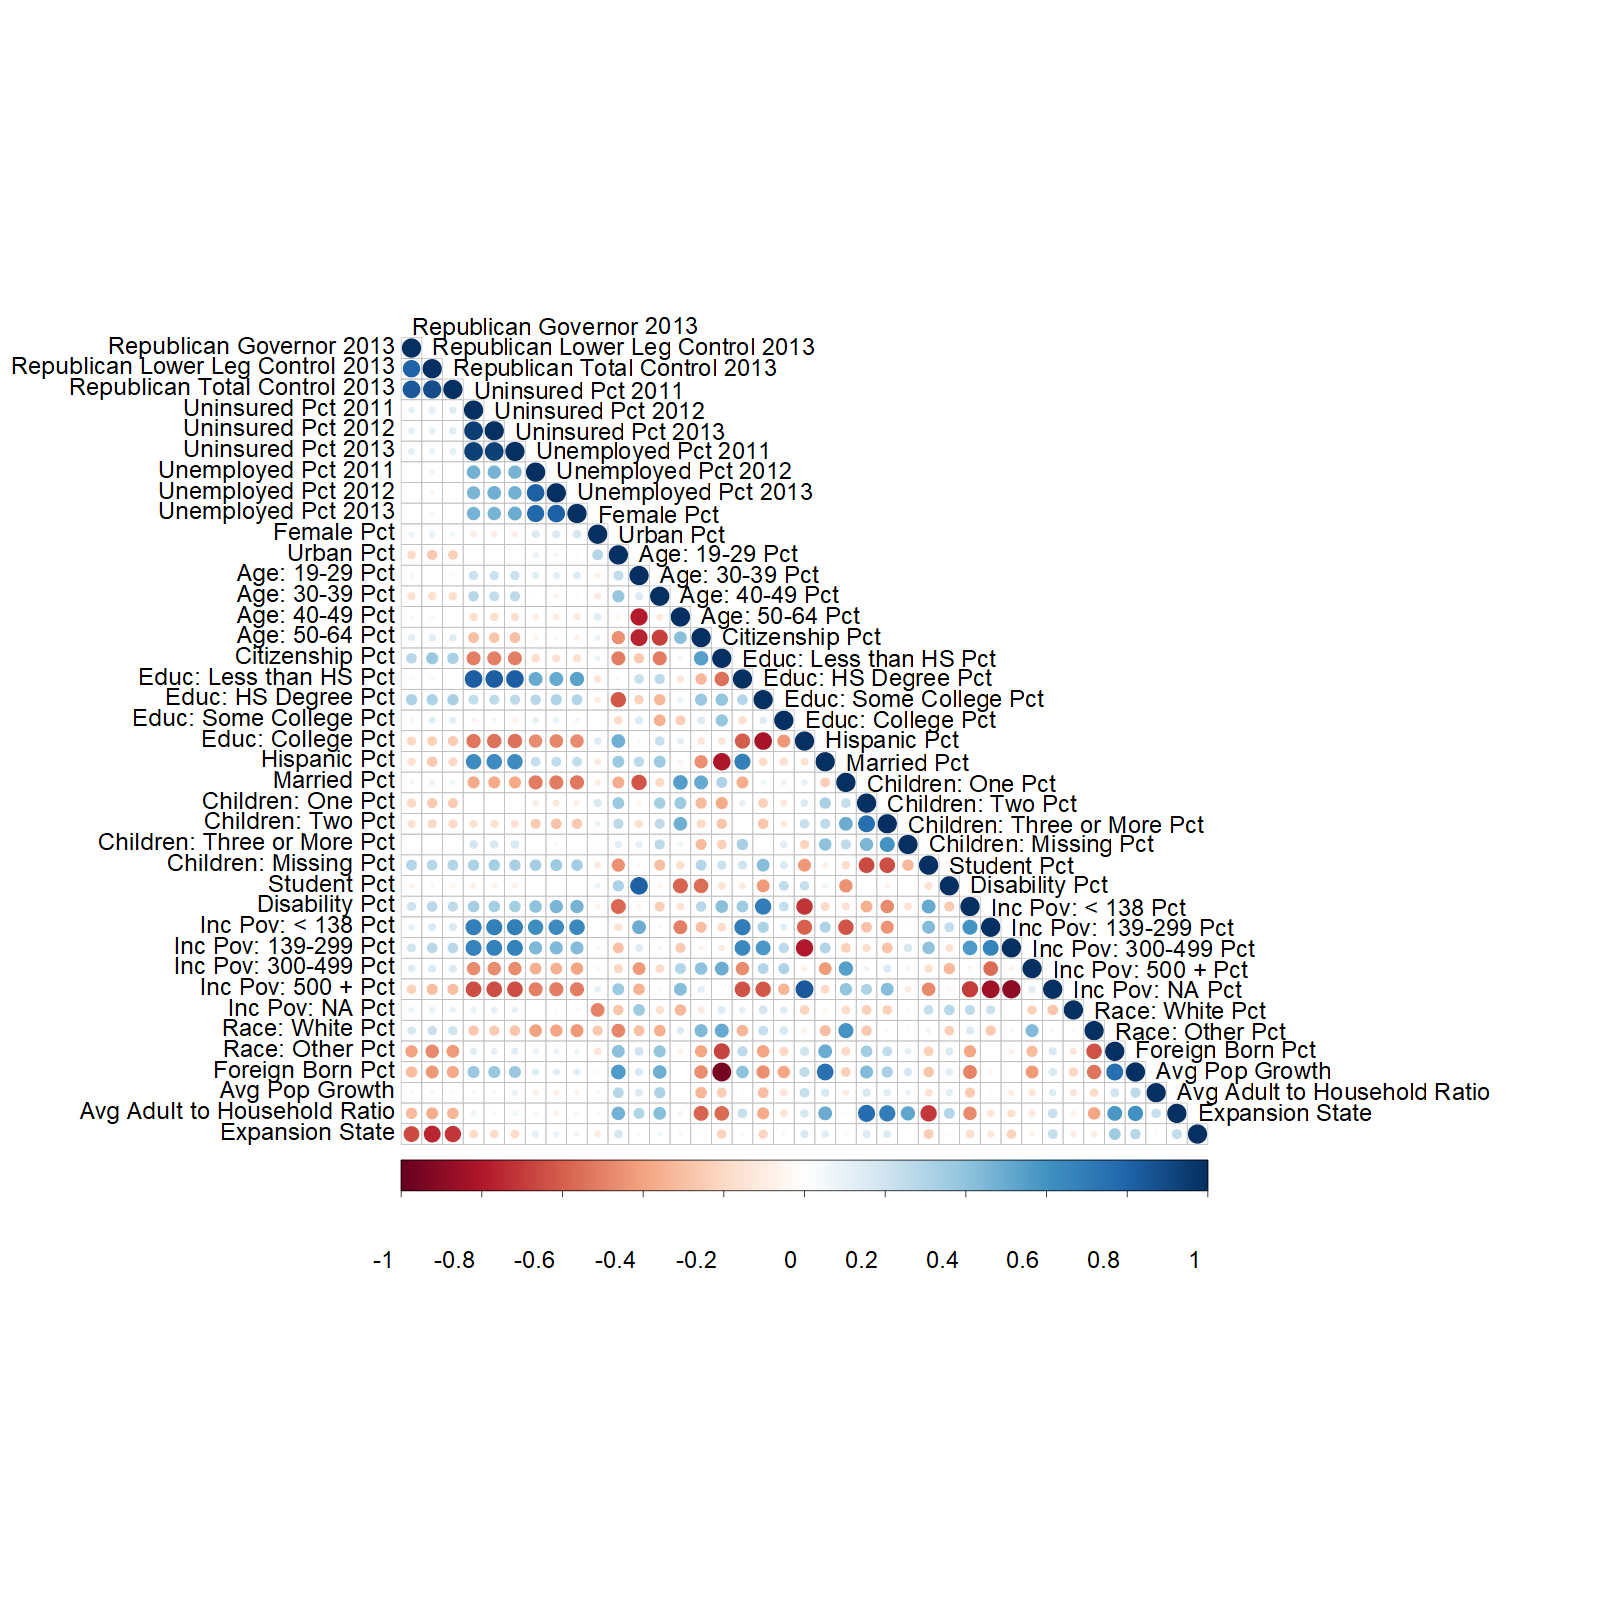
\includegraphics[scale=0.25]{01_Plots/correlation-plot-c1-sigma-zero.png}
\end{center}
\end{figure}

\clearpage

\clearpage

\section{Weight Diagnostics}\label{app:weightdiagnostics}

Table~\ref{tab:toltable} displays each covariate with the targeted level of maximal imbalance $\delta$ when generating approximate balancing weights. All variables and tolerances are measured in percentage points.

\begin{table}[ht]
\centering
\caption{Variables and maximal level of targeted imbalances ($\delta$)}
\begin{tabular}{lr}\label{tab:toltable}
Variable & $\delta$ \\ 
  \hline
Uninsured Pct 2011 & 0.05 \\ 
  Uninsured Pct 2012 & 0.05 \\ 
  Uninsured Pct 2013 & 0.05 \\ 
  Unemployed Pct 2011 & 0.15 \\ 
  Unemployed Pct 2012 & 0.15 \\ 
  Unemployed Pct 2013 & 0.15 \\ 
  Avg Pop Growth & 0.50 \\ 
  Avg Adult to Household Ratio & 0.50 \\ 
  Female Pct & 1.00 \\ 
  Age: 19-29 Pct & 1.00 \\ 
  Age: 30-39 Pct & 1.00 \\ 
  Age: 40-49 Pct & 1.00 \\ 
  Age: 50-64 Pct & 1.00 \\ 
  Married Pct & 1.00 \\ 
  Disability Pct & 1.00 \\ 
  Hispanic Pct & 1.00 \\ 
  Race: White Pct & 1.00 \\ 
  Children: One Pct & 1.00 \\ 
  Children: Two Pct & 1.00 \\ 
  Children: Three or More Pct & 1.00 \\ 
  Children: Missing Pct & 1.00 \\ 
  Urban Pct & 2.00 \\ 
  Citizenship Pct & 2.00 \\ 
  Educ: Less than HS Pct & 2.00 \\ 
  Educ: HS Degree Pct & 2.00 \\ 
  Educ: Some College Pct & 2.00 \\ 
  Educ: College Pct & 2.00 \\ 
  Student Pct & 2.00 \\ 
  Inc Pov: $<$ 138 Pct & 2.00 \\ 
  Inc Pov: 139-299 Pct & 2.00 \\ 
  Inc Pov: 300-499 Pct & 2.00 \\ 
  Inc Pov: 500 + Pct & 2.00 \\ 
  Inc Pov: NA Pct & 2.00 \\ 
  Race: Other Pct & 2.00 \\ 
  Foreign Born Pct & 2.00 \\ 
  Republican Governor 2013 & 25.00 \\ 
  Republican Lower Leg Control 2013 & 25.00 \\ 
  Republican Total Control 2013 & 25.00 \\ 
   \hline
\end{tabular}
\end{table}

\newpage

\begin{landscape}
Table~\ref{tab:baltab1} displays the differences between the weighted mean covariate values of the expansion region and the mean of the non-expansion region for our primary dataset and with the early expansion states excluded (calculated using our the homogeneous covariate adjustments). The weights presented here are for the H-SBW estimator. The values under each column are in the following format: (unweighted difference, weighted difference). ``Primary'' and ``Early excluded'' refer to the primary dataset and those that exclude the early expansion states. ``Percent'' indicates that the differences displayed are in percentage points while ``Standardized'' indicates that the standardized mean differences are displayed. Additional results are available on request.

\begin{table}[h!]\caption{Balance table: percent and standardized mean differences, H-SBW weights \\ (Weighted difference, Unweighted difference)}\label{tab:baltab1}
\centering
\begin{threeparttable}\begin{tabular}{lllll}
  \hline
Variables & Preferred (Percent) & Preferred (Standardized) & Early excluded (Percent) & Early excluded (Standardized) \\ 
  \hline
Age: 19-29 Pct & (-0.34, -0.34) & (-0.05, -0.05) & (-0.62, -0.21) & (-0.09, -0.03) \\ 
  Age: 30-39 Pct & (0.36, 0.17) & (0.1, 0.05) & (-0.04, 0.32) & (-0.01, 0.09) \\ 
  Age: 40-49 Pct & (0.19, -0.3) & (0.06, -0.1) & (-0.01, -0.44) & (0, -0.15) \\ 
  Avg Adult to Household Ratio & (11.29, -0.04) & (0.37, 0) & (3.37, 0.1) & (0.13, 0) \\ 
  Citizenship Pct & (-3.61, -1.59) & (-0.33, -0.15) & (-0.24, -1.45) & (-0.03, -0.16) \\ 
  Disability Pct & (-1.45, 0.52) & (-0.27, 0.1) & (-0.17, 0.63) & (-0.03, 0.11) \\ 
  Educ: HS Degree Pct & (-3.37, 0.54) & (-0.32, 0.05) & (-1.02, 0.64) & (-0.1, 0.06) \\ 
  Educ: Less than HS Pct & (-0.37, 0.83) & (-0.04, 0.1) & (-1.22, 0.76) & (-0.16, 0.1) \\ 
  Educ: Some College Pct & (-0.35, 0.4) & (-0.05, 0.06) & (0.36, 0.57) & (0.05, 0.08) \\ 
  Female Pct & (-0.34, -0.64) & (-0.16, -0.3) & (-0.25, -1) & (-0.12, -0.48) \\ 
  Foreign Born Pct & (7.6, 2) & (0.42, 0.11) & (1.02, 2) & (0.07, 0.13) \\ 
  Uninsured Pct 2011 & (-3.08, 0.05) & (-0.28, 0) & (-3.51, -0.05) & (-0.34, 0) \\ 
  Uninsured Pct 2012 & (-3, -0.05) & (-0.27, 0) & (-3.4, 0.05) & (-0.33, 0) \\ 
  Uninsured Pct 2013 & (-2.99, -0.05) & (-0.27, 0) & (-3.45, -0.05) & (-0.34, 0) \\ 
  Hispanic Pct & (4.46, 1) & (0.2, 0.04) & (-1.35, 1) & (-0.07, 0.05) \\ 
  Inc Pov: $<$ 138 Pct & (-2.05, 0.63) & (-0.19, 0.06) & (-1.33, 0.12) & (-0.12, 0.01) \\ 
  Inc Pov: 139-299 Pct & (-2.45, 0.65) & (-0.35, 0.09) & (-1.53, 0.5) & (-0.23, 0.08) \\ 
  Inc Pov: 300-499 Pct & (-0.59, -0.18) & (-0.12, -0.04) & (0.28, -0.18) & (0.06, -0.04) \\ 
  Inc Pov: 500 + Pct & (5.58, -1.3) & (0.35, -0.08) & (2.9, -1.23) & (0.2, -0.08) \\ 
  Married Pct & (-0.76, -0.43) & (-0.07, -0.04) & (-0.21, -0.53) & (-0.02, -0.05) \\ 
  Children: Missing Pct & (-3.25, -1) & (-0.36, -0.11) & (-1.99, -0.1) & (-0.21, -0.01) \\ 
  Children: One Pct & (0.7, -0.14) & (0.25, -0.05) & (0.11, -0.31) & (0.04, -0.12) \\ 
  Avg Pop Growth & (-0.09, -0.21) & (-0.07, -0.18) & (-0.26, -0.19) & (-0.22, -0.16) \\ 
  Race: White Pct & (-4.02, 1) & (-0.16, 0.04) & (0.09, 1) & (0, 0.04) \\ 
  Republican Governor 2013 & (-64.78, -25) & (-1.28, -0.5) & (-54.46, -24.87) & (-1.02, -0.47) \\ 
  Republican Lower Leg Control 2013 & (-74.72, -25) & (-1.69, -0.57) & (-56.67, -23.6) & (-1.12, -0.47) \\ 
  Republican Total Control 2013 & (-71.3, -25) & (-1.45, -0.51) & (-56.47, -25) & (-1.02, -0.45) \\ 
  Student Pct & (0.25, -0.5) & (0.04, -0.08) & (0.11, -0.25) & (0.02, -0.04) \\ 
  Children: Three or More Pct & (0, -0.21) & (0, -0.08) & (-0.17, -0.26) & (-0.07, -0.11) \\ 
  Children: Two Pct & (0.76, -0.31) & (0.23, -0.09) & (0.17, -0.37) & (0.05, -0.12) \\ 
  Unemployed Pct 2011 & (0.82, 0.15) & (0.18, 0.03) & (0.68, 0.15) & (0.15, 0.03) \\ 
  Unemployed Pct 2012 & (0.63, -0.03) & (0.14, -0.01) & (0.47, -0.03) & (0.11, -0.01) \\ 
  Unemployed Pct 2013 & (0.42, -0.15) & (0.11, -0.04) & (0.22, -0.15) & (0.06, -0.04) \\ 
  Urban Pct & (8.28, -2) & (0.26, -0.06) & (2.79, -2) & (0.08, -0.06) \\ 
   \hline
\end{tabular}
    \begin{tablenotes}
      \item[] The values displayed in each cell are the (weighted, unweighted) differences. The columns containing ``Standardized'' reflect the standardized mean differences while ``percent'' indicates the mean differences in percentage points. The columns containing ``Preferred'' indicate that this is for our primary analysis while ``Early excluded'' is for our analysis that excludes the early expansion states.
    \end{tablenotes}
\end{threeparttable}
\end{table}

\end{landscape}

Figure~\ref{fig:weightsbystatec1} shows the weights summed by states for the H-SBW, BC-HSBW, SBW, and BC-HSBW weights on the primary dataset. The positive and negative weights are displayed separately. Figure~\ref{fig:weightsbystatec2} displays the same plot excluding the early expansion states. These plots again show that H-SBW and BC-HSBW more evenly disperses the weights across states relative to SBW and BC-SBW, and also highlights the extent to which the weights extrapolate from each state for the bias-corrected estimators.

\begin{figure}[H]
\begin{center}
    \caption{Total weights summed by state, primary dataset}
    \label{fig:weightsbystatec1all}
    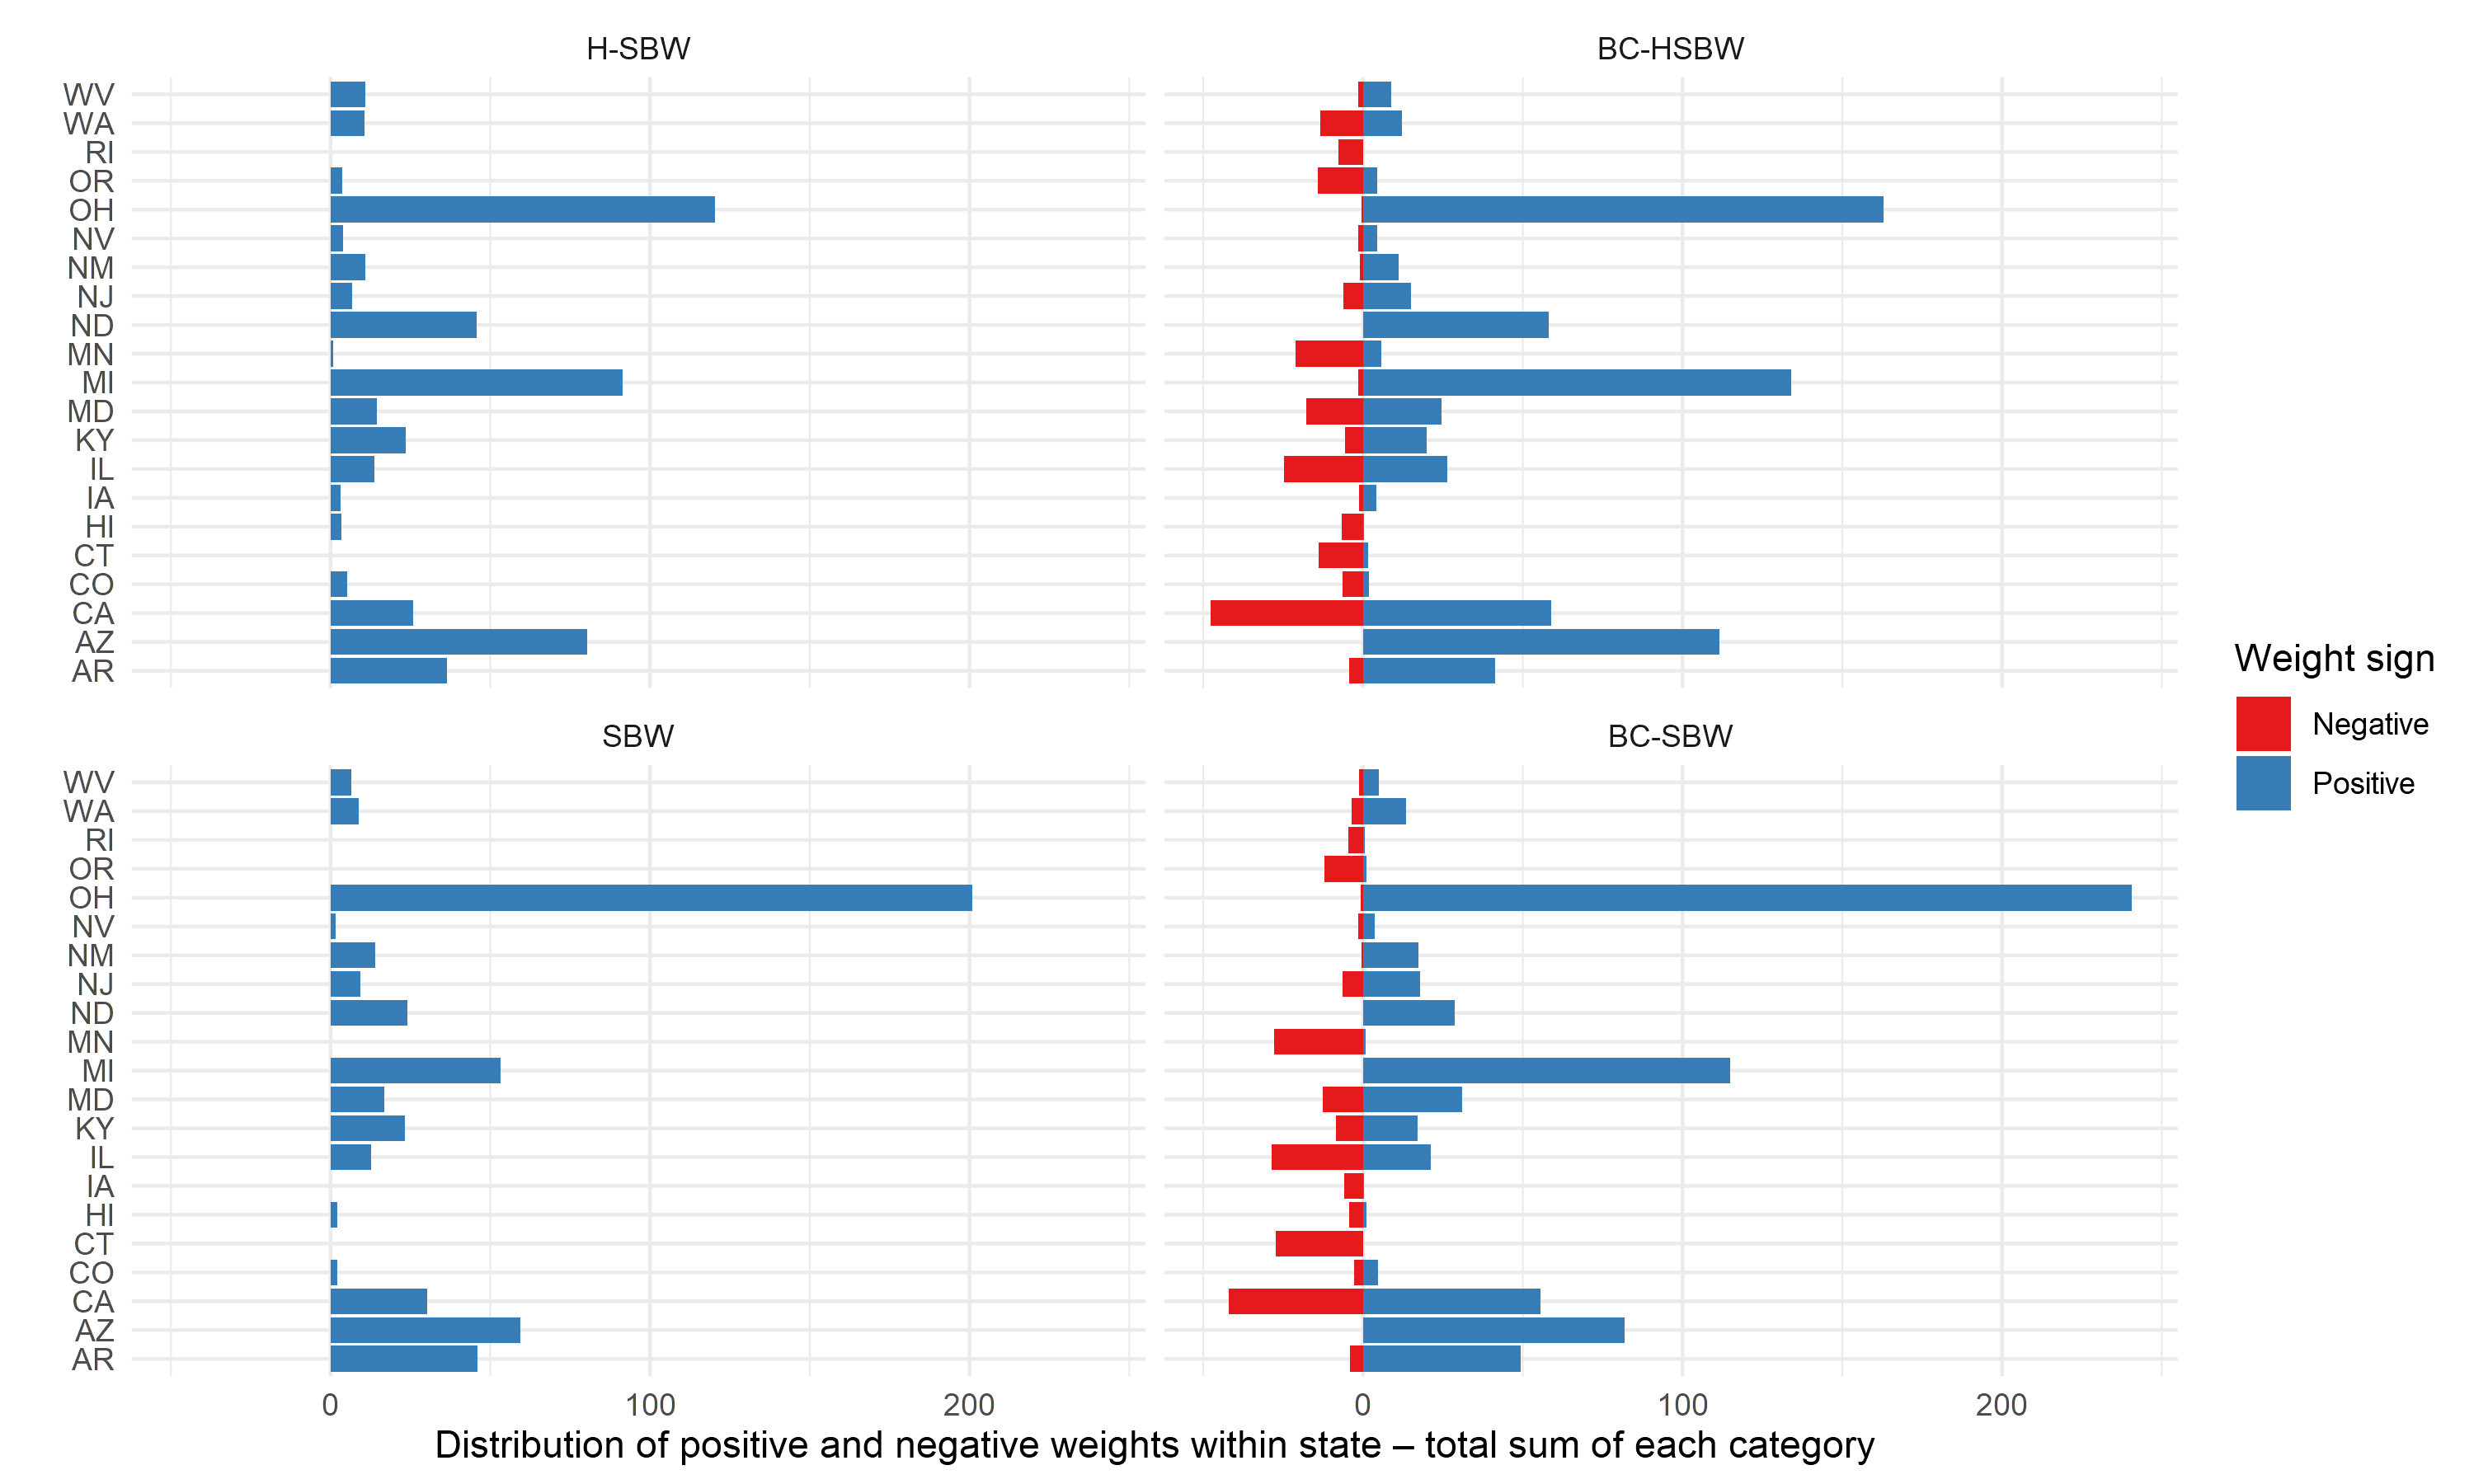
\includegraphics[scale=0.5]{01_Plots/weights-by-state-c1-all.png}
\end{center}
\end{figure}

\begin{figure}[H]
\begin{center}
    \caption{Total weights summed by state, early expansion excluded}
    \label{fig:weightsbystatec2all}
    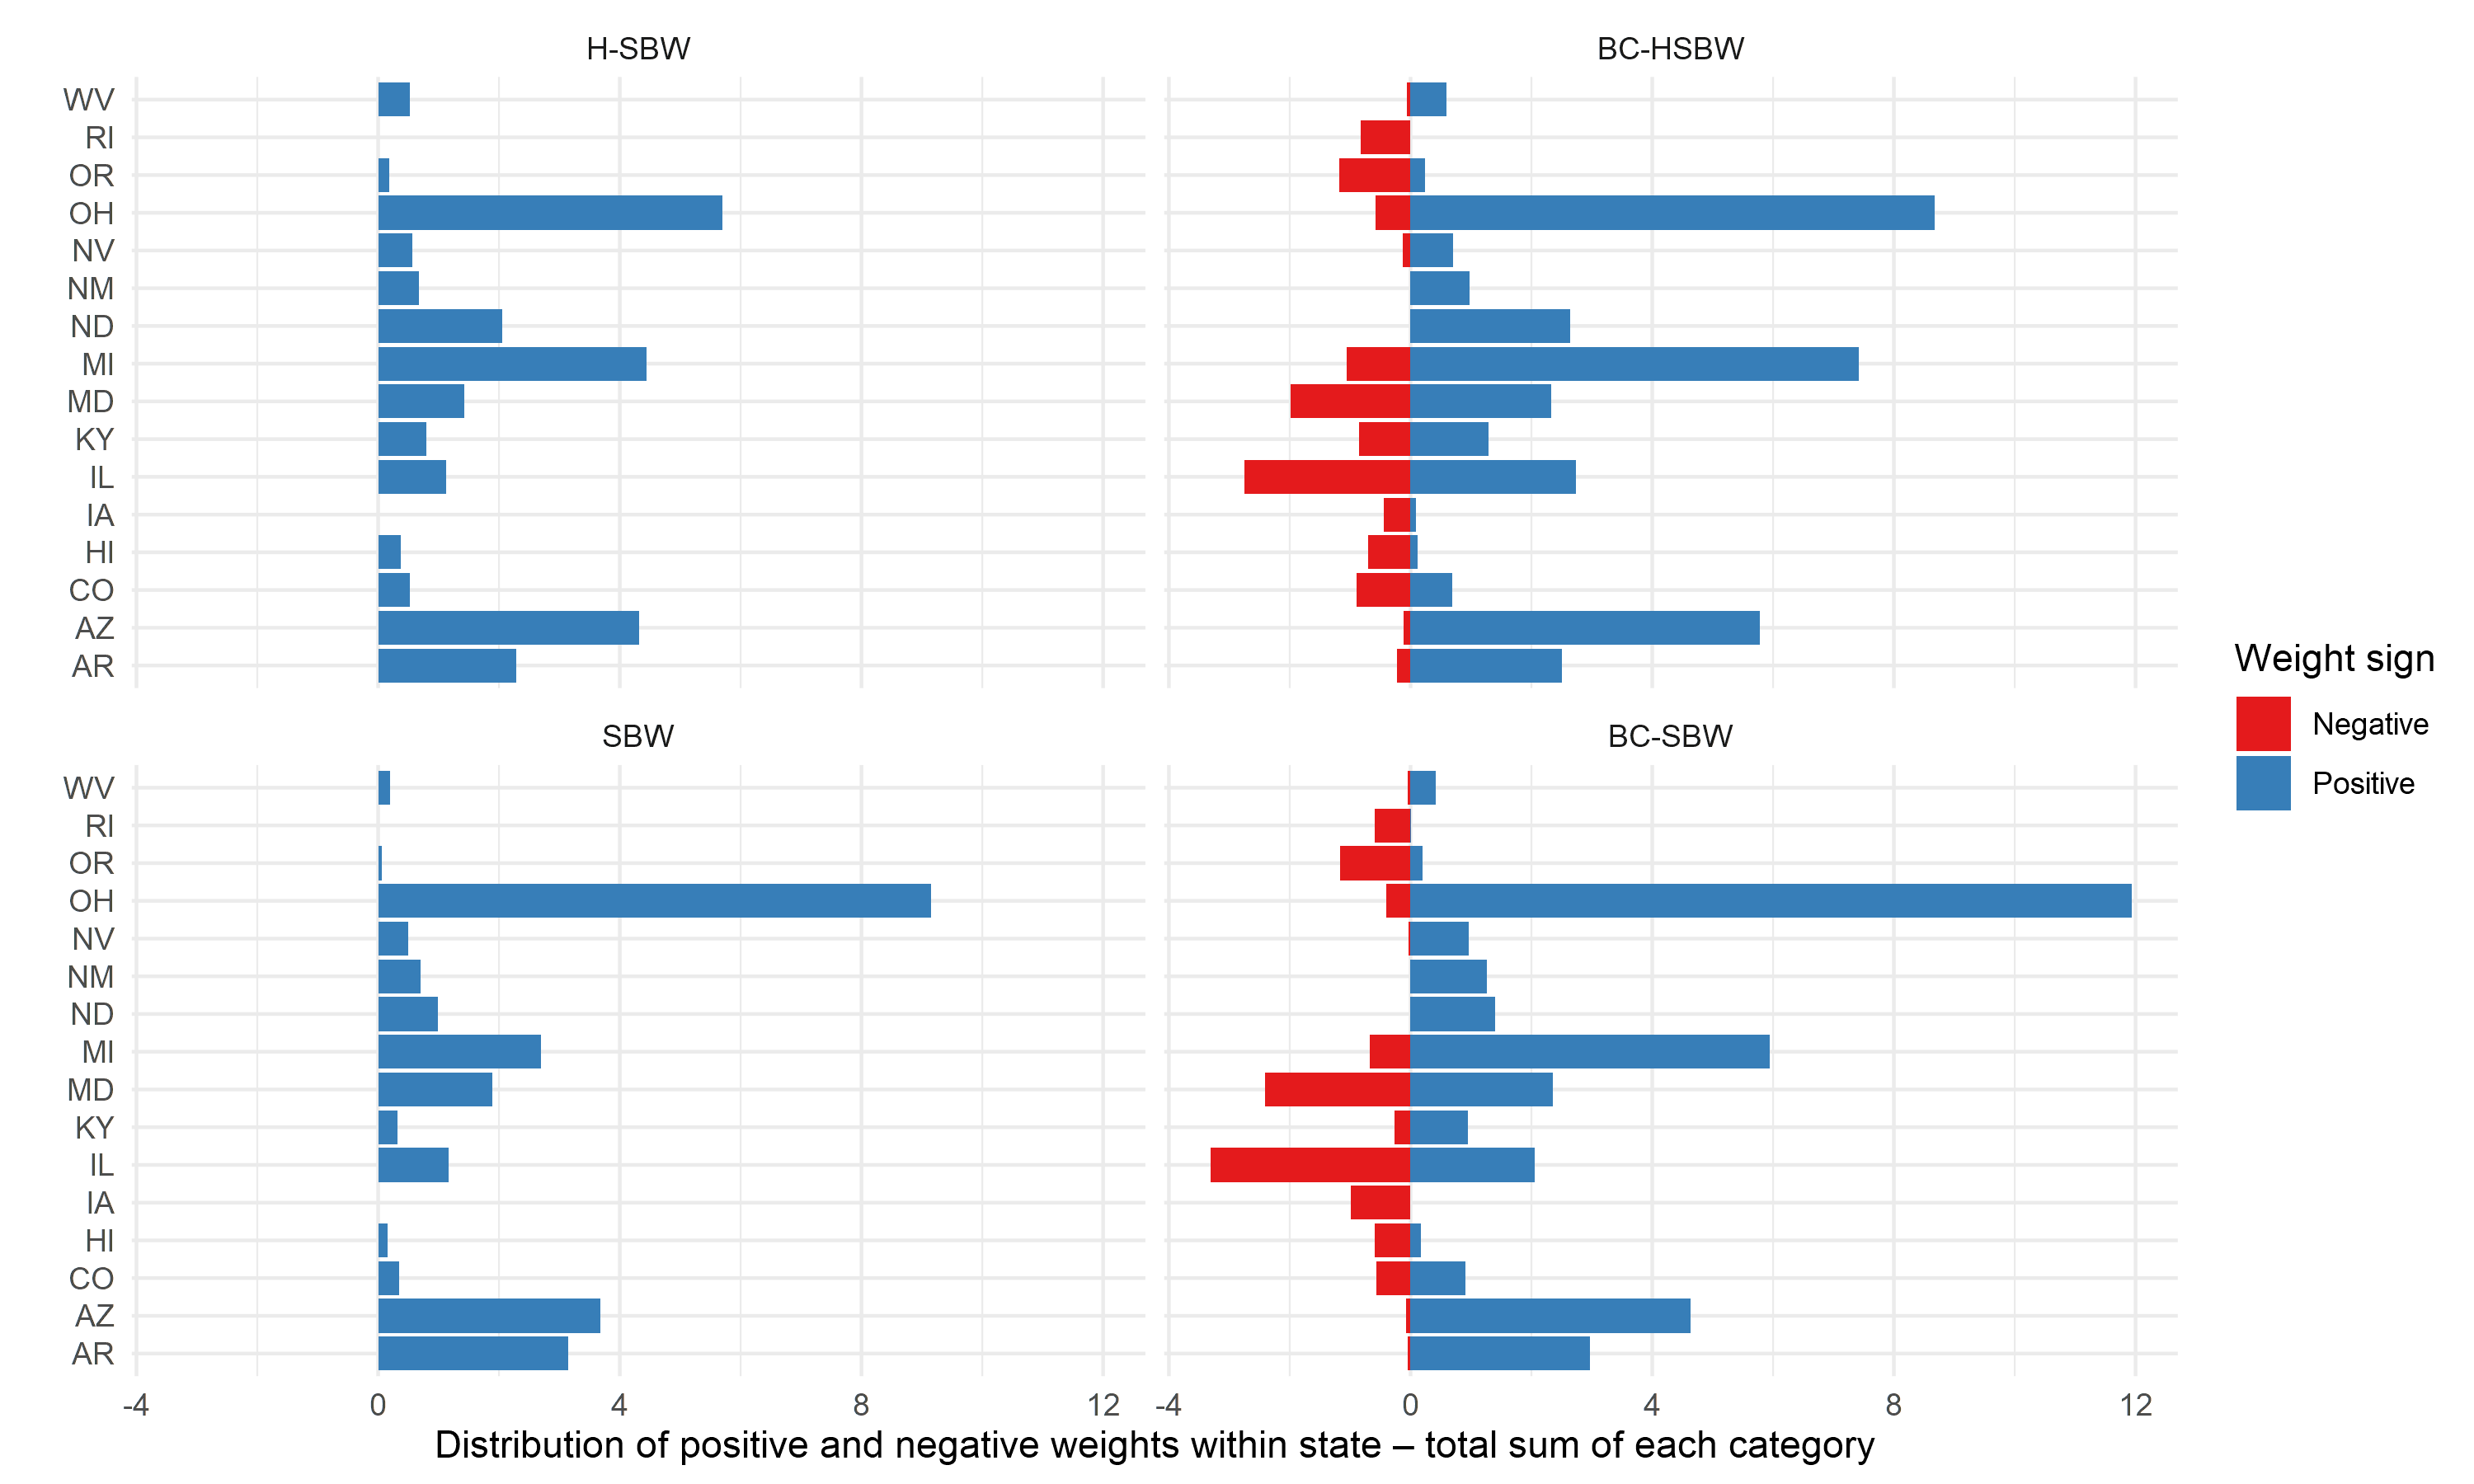
\includegraphics[scale=0.5]{01_Plots/weights-by-state-c2-all.png}
\end{center}
\end{figure}


We conclude by examining whether the H-SBW weights generated using the unadjusted data balance the adjusted covariates. While these metrics do not reflect the ``true'' imbalances, the comparison can provide some indication of whether the unadjusted weights are overfitting to noisy covariate measurements. Table~\ref{tab:balcomp} compares the imbalances among our pre-treatment outcomes using H-SBW weights generated on our unadjusted dataset applied to the adjusted (homogeneous) dataset. The ``Unweighted Difference'' column represents the raw difference in means, while the ``Weighted Difference'' column reflects the weighted difference that we calculate on the unadjusted dataset. The ``Homogeneous Diff'' column displays the weighted imbalance when applying the H-SBW weights to the dataset using the homogeneous adjustment, and similarly for ``Heterogeneous Diff.'' The weighted pre-treatment outcomes are approximately one percentage point lower than we desired in the two years prior to treatment using the heterogeneous adjustment, and -0.2 percentage points lower on average using the homogeneous adjustment. On the other hand, the naive difference suggests that the imbalance is only -0.05 percentage points. This result suggests that the unadjusted weights are overfitting to noisy covariates and may give an overly optimistic view of the covariate balance. Given the high degree of expected correlation between pre-treatment and post-treatment outcomes, we may expect the estimator of $\psi^1_0$ trained on the unadjusted data to have a negative bias.

\begin{table}[ht]
\caption{Balance comparison: weights estimated on unadjusted data applied to adjusted data}\label{tab:balcomp}
\begin{tabular}{lrrrr}
  \hline
Variables & Unweighted Diff & Weighted Difference & Homogeneous Diff & Heterogeneous Diff\\ 
  \hline
Uninsured Pct 2011 & -3.09 & -0.05 & -0.11 & 0.92 \\ 
  Uninsured Pct 2012 & -2.99 & -0.05 & -0.21 & -1.06 \\ 
  Uninsured Pct 2013 & -3.00 & -0.05 & -0.38 & -0.93 \\
  \hline
\end{tabular}
\end{table}
\clearpage

\clearpage

\section{Additional Results}
\label{ssec:allresults}

Table~\ref{tab:confintmain} displays the point estimates from all estimators as well as confidence intervals calculated either (a) leave-one-state-out jackknife on the adjusted dataset (CI (states)); (b) leave-one-state-out jackknife repeating the entire adjusted leaving each state out (CI (proc)). This table also includes all analyses calculated on a second version of the adjusted data where we use a common $\kappa$ for all values (sigma\_uu\_avg), which is the adjustment suggested by \cite{carroll2006measurement}. Notice that the confidence intervals are identical for ``sigma\_zero'' because this is the unadjusted dataset. ``sigma\_uu\_i'' is our preferred covariate adjustment.

\begin{table}[ht]
\centering
\caption{Point estimates and confidence intervals, primary dataset}
\label{tab:confintmain}
\begin{tabular}{llrll}
  \hline
Weight type & Sigma estimate & Psihat & CI (states) & CI (proc) \\ 
  \hline
H-SBW & sigma\_uu\_i & -2.17 & (-3.41, -0.94) & (-3.42, -0.92) \\ 
  H-SBW & sigma\_uu\_avg & -2.25 & (-3.51, -0.99) & (-3.35, -1.14) \\ 
  H-SBW & sigma\_zero & -2.35 & (-3.09, -1.61) & (-3.09, -1.61) \\ 
  BC-HSBW & sigma\_uu\_i & -2.13 & (-3.55, -0.71) & (-3.42, -0.84) \\ 
  BC-HSBW & sigma\_uu\_avg & -2.17 & (-3.57, -0.78) & (-3.39, -0.96) \\ 
  BC-HSBW & sigma\_zero & -2.40 & (-3.33, -1.46) & (-3.33, -1.46) \\ 
  SBW & sigma\_uu\_i & -2.24 & (-3.50, -0.99) & (-3.51, -0.97) \\ 
  SBW & sigma\_uu\_avg & -2.30 & (-3.67, -0.92) & (-3.45, -1.15) \\ 
  SBW & sigma\_zero & -2.40 & (-3.10, -1.69) & (-3.10, -1.69) \\ 
  BC-SBW & sigma\_uu\_i & -2.12 & (-3.15, -1.10) & (-3.11, -1.14) \\ 
  BC-SBW & sigma\_uu\_avg & -2.17 & (-3.25, -1.08) & (-3.22, -1.12) \\ 
  BC-SBW & sigma\_zero & -2.36 & (-2.93, -1.80) & (-2.93, -1.80) \\ 
   \hline
\end{tabular}
\end{table}

Table~\ref{tab:ptests} presents all point estimates from estimators that we calculated. The ``Var subset`` column indicates which variables were excluded from the estimation: 0 excludes no variables; 1 removes Republican governance indicators; 2 pre-treatment uninsurance and unemployment rates; 3 urban, age, education, citizenship, marital status, student, disability, or female; 4 race, ethnicity, income, foreign born; 5 children, population growth, and household to person ratio. We see that the largest changes generally occur when excluding the pre-treatment uninsurance and unemployment rates. This is not surprising: controlling for the other covariates, the pre-treatment uninsurance rate was substantially lower in the treated region compared to the control region. Given that pre-treatment uninsurance rates are highly correlated with post-treatment rates, we find that this comparison leads to a larger absolute magnitude point estimate, highlighting the need to control for these covariates.

%Wed Jan 13 15:24:43 2021
\begin{table}[ht]
\centering
\caption{Point estimates for all specifications}
\label{tab:ptests}
\begin{tabular}{rlrrrr}
  \hline
Variable subset & Sigma estimate & H-SBW & BC-HSBW & SBW & BC-SBW \\ 
  \hline
0 & sigma\_uu\_i & -2.17 & -2.13 & -2.24 & -2.12 \\ 
  0 & sigma\_uu\_avg & -2.25 & -2.17 & -2.30 & -2.17 \\ 
  0 & sigma\_zero & -2.35 & -2.40 & -2.40 & -2.36 \\ 
  1 & sigma\_uu\_i & -2.85 & -2.87 & -3.00 & -2.76 \\ 
  1 & sigma\_uu\_avg & -2.86 & -2.86 & -2.99 & -2.75 \\ 
  1 & sigma\_zero & -3.00 & -3.09 & -3.07 & -2.92 \\ 
  2 & sigma\_uu\_i & -5.73 & -5.05 & -5.24 & -4.70 \\ 
  2 & sigma\_uu\_avg & -5.73 & -5.05 & -5.24 & -4.70 \\ 
  2 & sigma\_zero & -5.73 & -5.13 & -5.24 & -4.77 \\ 
  3 & sigma\_uu\_i & -2.17 & -2.00 & -2.24 & -2.00 \\ 
  3 & sigma\_uu\_avg & -2.25 & -2.06 & -2.29 & -2.06 \\ 
  3 & sigma\_zero & -2.34 & -2.17 & -2.40 & -2.15 \\ 
  4 & sigma\_uu\_i & -2.35 & -2.39 & -2.29 & -2.30 \\ 
  4 & sigma\_uu\_avg & -2.39 & -2.39 & -2.32 & -2.32 \\ 
  4 & sigma\_zero & -2.45 & -2.59 & -2.43 & -2.49 \\ 
  5 & sigma\_uu\_i & -2.17 & -2.19 & -2.26 & -2.21 \\ 
  5 & sigma\_uu\_avg & -2.25 & -2.24 & -2.33 & -2.27 \\ 
  5 & sigma\_zero & -2.35 & -2.44 & -2.42 & -2.47 \\ 
   \hline
\end{tabular}
\end{table}

Table ~\ref{tab:confintmainc2} and Table~\ref{tab:secondaryptests} are identical to the structure of the previous two tables except we exclude the ``early expansion states'' from the pool of expansion state matches. 

\begin{table}[ht]
\centering
\caption{Point estimates and confidence intervals, early expansion excluded}
\label{tab:confintmainc2}
\begin{tabular}{llrll}
  \hline
Weight type & Sigma estimate & Psihat & CI (states) & CI (proc) \\ 
  \hline
H-SBW & sigma\_uu\_i & -2.05 & (-3.10, -1.00) & (-3.05, -1.05) \\ 
  H-SBW & sigma\_uu\_avg & -2.13 & (-3.20, -1.05) & (-3.17, -1.08) \\ 
  H-SBW & sigma\_zero & -2.29 & (-2.90, -1.69) & (-2.90, -1.69) \\ 
  BC-HSBW & sigma\_uu\_i & -2.14 & (-3.63, -0.64) & (-3.48, -0.80) \\ 
  BC-HSBW & sigma\_uu\_avg & -2.19 & (-3.65, -0.73) & (-3.57, -0.81) \\ 
  BC-HSBW & sigma\_zero & -2.50 & (-3.66, -1.33) & (-3.66, -1.33) \\ 
  SBW & sigma\_uu\_i & -1.91 & (-2.91, -0.91) & (-2.79, -1.03) \\ 
  SBW & sigma\_uu\_avg & -2.01 & (-3.02, -1.00) & (-2.83, -1.19) \\ 
  SBW & sigma\_zero & -2.20 & (-2.69, -1.71) & (-2.69, -1.71) \\ 
  BC-SBW & sigma\_uu\_i & -1.97 & (-3.49, -0.44) & (-3.27, -0.66) \\ 
  BC-SBW & sigma\_uu\_avg & -2.04 & (-3.59, -0.50) & (-3.39, -0.70) \\ 
  BC-SBW & sigma\_zero & -2.34 & (-3.44, -1.25) & (-3.44, -1.25) \\ 
   \hline
\end{tabular}
\end{table}

\begin{table}[ht]
\centering
   \caption{Point estimates for all specifications, early expansion excluded}
    \label{tab:secondaryptests}
\begin{tabular}{rlrrrr}
  \hline
Variable subset & Sigma estimate & H-SBW & BC-HSBW & SBW & BC-SBW \\ 
  \hline
0 & sigma\_uu\_i & -2.05 & -2.14 & -1.91 & -1.97 \\ 
  0 & sigma\_uu\_avg & -2.13 & -2.19 & -2.01 & -2.04 \\ 
  0 & sigma\_zero & -2.29 & -2.50 & -2.20 & -2.34 \\ 
  1 & sigma\_uu\_i & -2.85 & -2.99 & -2.85 & -2.86 \\ 
  1 & sigma\_uu\_avg & -2.86 & -2.98 & -2.86 & -2.86 \\ 
  1 & sigma\_zero & -3.05 & -3.18 & -2.96 & -2.99 \\ 
  2 & sigma\_uu\_i & -5.55 & -4.46 & -5.02 & -4.52 \\ 
  2 & sigma\_uu\_avg & -5.55 & -4.73 & -5.01 & -4.53 \\ 
  2 & sigma\_zero & -5.55 & -4.78 & -5.01 & -4.56 \\ 
  3 & sigma\_uu\_i & -2.05 & -2.03 & -1.91 & -1.89 \\ 
  3 & sigma\_uu\_avg & -2.13 & -2.10 & -2.00 & -1.97 \\ 
  3 & sigma\_zero & -2.27 & -2.22 & -2.20 & -2.13 \\ 
  4 & sigma\_uu\_i & -2.27 & -2.24 & -2.15 & -2.00 \\ 
  4 & sigma\_uu\_avg & -2.35 & -2.28 & -2.23 & -2.04 \\ 
  4 & sigma\_zero & -2.36 & -2.62 & -2.28 & -2.45 \\ 
  5 & sigma\_uu\_i & -2.05 & -2.20 & -1.91 & -2.03 \\ 
  5 & sigma\_uu\_avg & -2.13 & -2.26 & -1.99 & -2.11 \\ 
  5 & sigma\_zero & -2.29 & -2.45 & -2.19 & -2.36 \\ 
   \hline
\end{tabular}
\end{table}

Table~\ref{tab:loostatec1} and Table~\ref{tab:loostatec2} present point estimates for the leave-one-state out analysis for our preferred estimator, H-SBW calculated on our preferred covariate adjustment for the primary dataset and when excluding early expansion states.

\begin{table}[ht]
\centering
   \caption{Leave-one-state-out point estimates, primary dataset, preferred adjustment}
    \label{tab:loostatec1}
\begin{tabular}{lrlrl}
  \hline
State & Psihat (0) & None (states, proc) & Psihat (1) & Repub (states, proc) \\ 
  \hline
AR & -2.17 & (-2.34, -2.38) & -2.85 & (-2.81, -2.80) \\ 
  AZ & -2.17 & (-2.21, -2.24) & -2.85 & (-2.86, -2.86) \\ 
  CA & -2.17 & (-1.99, -2.02) & -2.85 & (-2.77, -2.76) \\ 
  CO & -2.17 & (-2.17, -2.23) & -2.85 & (-2.84, -2.84) \\ 
  CT & -2.17 & (-2.17, -2.15) & -2.85 & (-2.83, -2.82) \\ 
  HI & -2.17 & (-2.15, -2.14) & -2.85 & (-2.77, -2.78) \\ 
  IA & -2.17 & (-2.09, -2.07) & -2.85 & (-2.83, -2.84) \\ 
  IL & -2.17 & (-2.16, -2.24) & -2.85 & (-2.83, -2.84) \\ 
  KY & -2.17 & (-2.02, -1.95) & -2.85 & (-2.57, -2.52) \\ 
  MD & -2.17 & (-2.25, -2.27) & -2.85 & (-2.94, -2.94) \\ 
  MI & -2.17 & (-2.10, -2.18) & -2.85 & (-2.89, -2.92) \\ 
  MN & -2.17 & (-2.17, -2.19) & -2.85 & (-2.84, -2.86) \\ 
  ND & -2.17 & (-2.23, -2.26) & -2.85 & (-2.84, -2.84) \\ 
  NH & -2.17 & (-2.18, -2.21) & -2.85 & (-2.98, -2.99) \\ 
  NJ & -2.17 & (-2.26, -2.25) & -2.85 & (-2.99, -3.03) \\ 
  NM & -2.17 & (-2.16, -2.22) & -2.85 & (-2.76, -2.77) \\ 
  NV & -2.17 & (-2.21, -2.24) & -2.85 & (-2.89, -2.88) \\ 
  OH & -2.17 & (-2.70, -2.68) & -2.85 & (-3.00, -2.98) \\ 
  OR & -2.17 & (-2.17, -2.25) & -2.85 & (-2.80, -2.84) \\ 
  RI & -2.17 & (-2.17, -2.15) & -2.85 & (-2.81, -2.81) \\ 
  WA & -2.17 & (-2.10, -2.11) & -2.85 & (-2.78, -2.77) \\ 
  WV & -2.17 & (-2.16, -2.18) & -2.85 & (-2.8, -2.78) \\ 
   \hline
\end{tabular}
\end{table}

\begin{table}[ht]
\centering
   \caption{Leave-one-state-out point estimates, early expansion excluded, preferred adjustment}
    \label{tab:loostatec2}
\begin{tabular}{lrlrl}
  \hline
State & Psihat (0) & None (states, proc) & Psihat (1) & Repub (states, proc) \\ 
  \hline
AR & -2.05 & (-2.15, -2.16) & -2.85 & (-2.77, -2.76) \\ 
  AZ & -2.05 & (-1.82, -1.88) & -2.85 & (-2.87, -2.86) \\ 
  CO & -2.05 & (-2.07, -2.09) & -2.85 & (-2.84, -2.83) \\ 
  HI & -2.05 & (-2.01, -1.99) & -2.85 & (-2.71, -2.73) \\ 
  IA & -2.05 & (-1.98, -1.95) & -2.85 & (-2.85, -2.86) \\ 
  IL & -2.05 & (-2.03, -2.01) & -2.85 & (-2.8, -2.79) \\ 
  KY & -2.05 & (-1.87, -1.8) & -2.85 & (-2.59, -2.54) \\ 
  MD & -2.05 & (-2.18, -2.15) & -2.85 & (-2.97, -2.96) \\ 
  MI & -2.05 & (-1.96, -2) & -2.85 & (-2.92, -2.96) \\ 
  ND & -2.05 & (-2.02, -2.04) & -2.85 & (-2.84, -2.84) \\ 
  NH & -2.05 & (-2.05, -2.06) & -2.85 & (-3.02, -3.03) \\ 
  NM & -2.05 & (-1.99, -1.97) & -2.85 & (-2.72, -2.75) \\ 
  NV & -2.05 & (-2.15, -2.15) & -2.85 & (-2.93, -2.92) \\ 
  OH & -2.05 & (-2.43, -2.38) & -2.85 & (-3.03, -3.02) \\ 
  OR & -2.05 & (-2.05, -2.11) & -2.85 & (-2.81, -2.84) \\ 
  RI & -2.05 & (-2.05, -2.05) & -2.85 & (-2.80, -2.80) \\ 
  WV & -2.05 & (-2.06, -2.06) & -2.85 & (-2.83, -2.81) \\ 
   \hline
\end{tabular}
\end{table}

Table~\ref{tab:oateconfint} displays point estimates and confidence intervals for the primary point estimates for the OATE. We display the confidence intervals calculated using both the leave-one-out-states conditional on the covariate adjustment (CI (states)) and recalculating the covariate adjustment for the OATE (CI (proc)). 

\begin{table}[ht]
\centering
\caption{OATE primary results inference}
\label{tab:oateconfint}
\begin{tabular}{rllll}
  \hline
Psihat & Sigma estimate & Dataset & CI (states) & CI (proc) \\ 
  \hline
-1.74 & sigma\_uu\_i\_modeled & c1 & (-2.35, -1.14) & (-2.48, -1.00) \\ 
  -1.67 & sigma\_uu\_avg & c1 & (-2.34, -0.99) & (-2.52, -0.81) \\ 
  -1.80 & sigma\_zero & c1 & (-2.50, -1.10) & (-2.50, -1.10) \\ 
  -1.89 & sigma\_uu\_i\_modeled & c2 & (-2.47, -1.32) & (-2.54, -1.24) \\ 
  -1.80 & sigma\_uu\_avg & c2 & (-2.43, -1.17) & (-2.57, -1.03) \\ 
  -1.95 & sigma\_zero & c2 & (-2.65, -1.25) & (-2.65, -1.25) \\ 
   \hline
\end{tabular}
\end{table}

Table~\ref{tab:oatesensitive} presents all point estimates calculate using the overlap weights. Dataset ``c1'' refers to the primary dataset and dataset ``c2'' removes the early expansion states. The numeric column names refer to the covariate group excluded (covariate groups described above).

\begin{table}[ht]
\centering
\caption{OATE all point estimates}
\label{tab:oatesensitive}
\begin{tabular}{llrrrrrr}
  \hline
Sigma estimate & Dataset & 0 & 1 & 2 & 3 & 4 & 5 \\ 
  \hline
sigma\_uu\_i & c1 & -1.64 & -2.60 & -2.96 & -1.86 & -1.86 & -1.77 \\ 
  sigma\_uu\_i & c2 & -1.81 & -2.53 & -3.10 & -2.18 & -2.04 & -1.96 \\ 
  sigma\_avg & c1 & -1.58 & -2.62 & -2.85 & -1.76 & -1.76 & -1.78 \\ 
  sigma\_avg & c2 & -1.74 & -2.54 & -3.00 & -2.10 & -1.96 & -1.95 \\ 
  sigma\_zero & c1 & -1.80 & -2.55 & -3.11 & -1.98 & -1.94 & -1.83 \\ 
  sigma\_zero & c2 & -1.95 & -2.51 & -3.25 & -2.12 & -2.10 & -2.00 \\ 
   \hline
\end{tabular}
\end{table}

Table~\ref{tab:rdiffc1} and ~\ref{tab:rdiffc2} display the quantiles of the distribution $\hat{\Delta}_v^1$ estimates when leaving out each state for the primary dataset and removing the early expansion states. The ``resample'' column indicates whether the entire adjustment procedure was recalculated (``proc'') or whether we left out each state conditional on the adjustment (``states''). Table~\ref{tab:hte} displays the estimated linear combination of model coefficients on the Republican governance indicators with 95 percent confidence intervals (standard errors clustered at the state level). The ``Weights'' column represents whether the regressions were weighted; we ran two versions, an unweighted regression and one using the overlap weights.

\begin{table}[ht]
\centering
\label{tab:rdiffc1}
\caption{$\hat{\Delta}^1_v$ leave-one-state-out estimates, primary dataset}
\begin{tabular}{lllrrrrrr}
  \hline
Resample & Sigma estimate & Weight type & Original & 0\% & 25\% & 50\% & 75\% & 100\% \\ 
  \hline
states & sigma\_uu\_i\_modeled & H-SBW & -0.67 & -0.80 & -0.68 & -0.67 & -0.62 & -0.30 \\ 
  proc & sigma\_uu\_i\_modeled & H-SBW & -0.67 & -0.78 & -0.68 & -0.64 & -0.59 & -0.30 \\ 
  states & sigma\_uu\_i\_modeled & BC-HSBW & -0.74 & -0.87 & -0.77 & -0.71 & -0.69 & -0.26 \\ 
  proc & sigma\_uu\_i\_modeled & BC-HSBW & -0.74 & -0.85 & -0.76 & -0.70 & -0.67 & -0.34 \\ 
  states & sigma\_uu\_i\_modeled & SBW & -0.75 & -0.98 & -0.77 & -0.75 & -0.72 & -0.48 \\ 
  proc & sigma\_uu\_i\_modeled & SBW & -0.75 & -0.98 & -0.78 & -0.73 & -0.67 & -0.49 \\ 
  states & sigma\_uu\_i\_modeled & BC-SBW & -0.63 & -0.85 & -0.69 & -0.62 & -0.61 & -0.39 \\ 
  proc & sigma\_uu\_i\_modeled & BC-SBW & -0.63 & -0.82 & -0.68 & -0.64 & -0.59 & -0.35 \\ 
  states & sigma\_uu\_avg & H-SBW & -0.61 & -0.74 & -0.64 & -0.60 & -0.57 & -0.23 \\ 
  proc & sigma\_uu\_avg & H-SBW & -0.61 & -0.76 & -0.63 & -0.59 & -0.55 & -0.33 \\ 
  states & sigma\_uu\_avg & BC-HSBW & -0.69 & -0.83 & -0.73 & -0.68 & -0.64 & -0.24 \\ 
  proc & sigma\_uu\_avg & BC-HSBW & -0.69 & -0.83 & -0.73 & -0.66 & -0.63 & -0.39 \\ 
  states & sigma\_uu\_avg & SBW & -0.70 & -0.89 & -0.72 & -0.69 & -0.67 & -0.31 \\ 
  proc & sigma\_uu\_avg & SBW & -0.70 & -0.93 & -0.73 & -0.68 & -0.65 & -0.49 \\ 
  states & sigma\_uu\_avg & BC-SBW & -0.58 & -0.78 & -0.63 & -0.57 & -0.56 & -0.32 \\ 
  proc & sigma\_uu\_avg & BC-SBW & -0.58 & -0.81 & -0.63 & -0.58 & -0.55 & -0.28 \\ 
  states & sigma\_zero & H-SBW & -0.65 & -0.78 & -0.66 & -0.63 & -0.61 & -0.50 \\ 
  proc & sigma\_zero & H-SBW & -0.65 & -0.78 & -0.66 & -0.63 & -0.61 & -0.50 \\ 
  states & sigma\_zero & BC-HSBW & -0.70 & -0.88 & -0.74 & -0.68 & -0.64 & -0.50 \\ 
  proc & sigma\_zero & BC-HSBW & -0.70 & -0.88 & -0.74 & -0.68 & -0.64 & -0.50 \\ 
  states & sigma\_zero & SBW & -0.68 & -0.84 & -0.71 & -0.68 & -0.66 & -0.49 \\ 
  proc & sigma\_zero & SBW & -0.68 & -0.84 & -0.71 & -0.68 & -0.66 & -0.49 \\ 
  states & sigma\_zero & BC-SBW & -0.56 & -0.67 & -0.61 & -0.55 & -0.52 & -0.39 \\ 
  proc & sigma\_zero & BC-SBW & -0.56 & -0.67 & -0.61 & -0.55 & -0.52 & -0.39 \\ 
   \hline
\end{tabular}
\end{table}

\begin{table}[ht]
\label{tab:rdiffc2}
\caption{$\hat{\Delta}^1_v$ leave-one-state-out estimates, early expansion excluded}
\centering
\begin{tabular}{lllrrrrrr}
  \hline
Resample & Sigma estimate & Weight type & Original & 0\% & 25\% & 50\% & 75\% & 100\% \\ 
  \hline
states & sigma\_uu\_i\_modeled & H-SBW & -0.80 & -1.05 & -0.82 & -0.77 & -0.73 & -0.60 \\ 
  proc & sigma\_uu\_i\_modeled & H-SBW & -0.80 & -0.98 & -0.81 & -0.76 & -0.74 & -0.60 \\ 
  states & sigma\_uu\_i\_modeled & BC-HSBW & -0.85 & -1.13 & -0.96 & -0.83 & -0.76 & -0.45 \\ 
  proc & sigma\_uu\_i\_modeled & BC-HSBW & -0.85 & -1.05 & -0.94 & -0.83 & -0.77 & -0.53 \\ 
  states & sigma\_uu\_i\_modeled & SBW & -0.94 & -1.15 & -0.94 & -0.92 & -0.89 & -0.70 \\ 
  proc & sigma\_uu\_i\_modeled & SBW & -0.94 & -1.05 & -0.98 & -0.91 & -0.86 & -0.73 \\ 
  states & sigma\_uu\_i\_modeled & BC-SBW & -0.89 & -1.27 & -0.93 & -0.86 & -0.81 & -0.26 \\ 
  proc & sigma\_uu\_i\_modeled & BC-SBW & -0.89 & -1.19 & -0.96 & -0.86 & -0.81 & -0.37 \\ 
  states & sigma\_uu\_avg & H-SBW & -0.73 & -0.99 & -0.74 & -0.70 & -0.68 & -0.51 \\ 
  proc & sigma\_uu\_avg & H-SBW & -0.73 & -0.94 & -0.73 & -0.69 & -0.67 & -0.50 \\ 
  states & sigma\_uu\_avg & BC-HSBW & -0.79 & -1.10 & -0.87 & -0.78 & -0.69 & -0.42 \\ 
  proc & sigma\_uu\_avg & BC-HSBW & -0.79 & -1.01 & -0.89 & -0.73 & -0.69 & -0.46 \\ 
  states & sigma\_uu\_avg & SBW & -0.85 & -1.08 & -0.85 & -0.83 & -0.81 & -0.66 \\ 
  proc & sigma\_uu\_avg & SBW & -0.85 & -0.95 & -0.86 & -0.82 & -0.80 & -0.68 \\ 
  states & sigma\_uu\_avg & BC-SBW & -0.82 & -1.21 & -0.86 & -0.80 & -0.74 & -0.18 \\ 
  proc & sigma\_uu\_avg & BC-SBW & -0.82 & -1.09 & -0.86 & -0.76 & -0.74 & -0.26 \\ 
  states & sigma\_zero & H-SBW & -0.76 & -0.95 & -0.83 & -0.74 & -0.70 & -0.58 \\ 
  proc & sigma\_zero & H-SBW & -0.76 & -0.95 & -0.83 & -0.74 & -0.70 & -0.58 \\ 
  states & sigma\_zero & BC-HSBW & -0.69 & -1.00 & -0.83 & -0.70 & -0.60 & -0.39 \\ 
  proc & sigma\_zero & BC-HSBW & -0.69 & -1.00 & -0.83 & -0.70 & -0.60 & -0.39 \\ 
  states & sigma\_zero & SBW & -0.76 & -0.91 & -0.83 & -0.75 & -0.74 & -0.51 \\ 
  proc & sigma\_zero & SBW & -0.76 & -0.91 & -0.83 & -0.75 & -0.74 & -0.51 \\ 
  states & sigma\_zero & BC-SBW & -0.64 & -1.06 & -0.70 & -0.58 & -0.55 & -0.38 \\ 
  proc & sigma\_zero & BC-SBW & -0.64 & -1.06 & -0.70 & -0.58 & -0.55 & -0.38 \\ 
   \hline
\end{tabular}
\end{table}

\begin{table}[ht]
\caption{OLS HTE estimates}
\label{tab:hte}
\centering
\begin{tabular}{rllll}
  \hline
Estimate & Dataset & Sigma estimate & CI 95 & Weights \\ 
  \hline
  -1.76 & c1 & sigma\_uu\_i\_modeled & (-5.47, 1.94) & Overlap \\ 
  -1.67 & c1 & sigma\_uu\_avg & (-7.18, 3.84) & Overlap \\ 
  -1.97 & c1 & sigma\_zero & (-4.11, 0.17) & Overlap \\ 
  0.51 & c2 & sigma\_uu\_i\_modeled & (-6.00, 7.02) & Overlap \\ 
  -0.17 & c2 & sigma\_uu\_avg & (-8.17, 7.83) & Overlap \\ 
  -1.48 & c2 & sigma\_zero & (-3.51, 0.54) & Overlap \\ 
  0.10 & c1 & sigma\_uu\_i\_modeled & (-1.09, 1.30) & None \\ 
  0.61 & c1 & sigma\_uu\_avg & (-1.82, 3.04) & None \\ 
  -0.12 & c1 & sigma\_zero & (-0.90, 0.66) & None \\ 
  0.37 & c2 & sigma\_uu\_i\_modeled & (-0.9, 1.63) & None \\ 
  0.64 & c2 & sigma\_uu\_avg & (-1.77, 3.04) & None \\ 
  -0.11 & c2 & sigma\_zero & (-0.91, 0.68) & None \\ 
   \hline
\end{tabular}
\end{table}


\clearpage

\section{Simulation Study}\label{app:simstudy}

This section presents a simulation study evaluating the performance of our proposed estimators on a known data-generating process. The first subsection outlines our simulation study. The section section presents selected results about the bias and mean-square error of our estimators, and the coverage rates for our proposed variance estimation procedure.

\subsection{Study design}

We first generate data according to a known and evaluate the performance of different estimators. For all models we consider the data generating process:

\begin{align*}
Y_{sc} \sim N(X_{1, sc} + X_{2, sc} + X_{3, sc}, \sigma^2_{\epsilon} + \sigma^2_{\varepsilon})
\end{align*}

where $\sigma^2_{\varepsilon}$ represents the variance component from a state-level random effect, and $\sigma^2_{\epsilon}$ represents a variance component from a CPUMA-level random effect. Thus the errors in the model for $Y \mid X$ are equicorrelated within state with correlation $\rho$ equal to $\frac{\sigma^2_{\varepsilon}}{\sigma^2_{\epsilon} + \sigma^2_{\varepsilon}}$

We next define a correlation structure among our observed covariates. Specifically, we generate each covariate vector $X_{sc}$:

\begin{align*}
X_{sc} \sim N(\mu_s, \Sigma_{Q}) \\
\mu_j \sim N(0, \Sigma_{S}) \\
\end{align*}

Define $\Sigma_X = \Sigma_Q + \Sigma_S$. Let $\sigma^2_{x, j}$ be the j-th diagonal element of $\Sigma_X$ (and define $\sigma^2_{q, j}$ and $\sigma^2_{s, j}$ analogously). Across all simulations, we fix $\sigma^2_{x, j} = 2$. We also fix the off-diagonal elements of both $\Sigma_Q$ and $\Sigma_S$ to be equal and so that $Cor(X_j, X_k) = 0.25$. Finally, define $\rho_x = Cor(X_{sc}, X_{sd})$ for $c \ne d$; in other words, $\rho_x$ is the within-state correlation of the covariates $X_{sc}$, which we set to be equal for all covariates.

We also consider samples of size $m = 25$ states each with $p_s$ units and $n$ total units. We draw $p_s \stackrel{iid}\sim \lfloor Exp(0.1) + 10\rfloor$ so that the average number of regions per state is approximately 20 (and the approximate number of total units $n$ is on average approximately 450).

We next generate our noisy outcome and covariate estimates $(J, W)$:

\begin{align*}
(J_{sc}, W_{sc}) \stackrel{iid}\sim N((Y_{sc}, X_{sc}), \Sigma_{\nu, sc})
\end{align*}

\begin{align*}
    \Sigma_{\nu} = \begin{pmatrix}
    \sigma^2_{\nu, sc} & 0 & 0 & 0 \\
    0 & \sigma^2_{\nu, sc} & 0 & 0 \\
    0 & 0 & \sigma^2_{\nu, sc} & 0 \\
    0 & 0 & 0 & \sigma^2_{\nu, sc}
    \end{pmatrix}
\end{align*}

First, define $\rho_y = \sigma^2_{\varepsilon}/(\sigma^2_{\epsilon} + \sigma^2_{\varepsilon} + \sigma^2_{\nu})$. In other words, $\rho_y$ represents the within-state correlation of the outcome model errors, including the measurement errors in the outcome. We fix this to be 0.25 throughout all simulations.

We allow $\sigma^2_{\nu, sc}$ to be a function of the sample size of an underlying survey that generates the estimate. We simulate these sample sizes $r_{sc}$ drawn from some distribution (see more on this below). Let $R_{sc}$ be a 3x3 diagonal matrix with diagonal elements $r_{sc}$. Let $\sigma_{\nu}^{2\star}$ be defined as the limit as $n \to \infty$ of $n^{-1}\sum_{sc}\sigma^2_{\nu, sc}$ (we ensure this limit exists). Let $\tau = \sigma^2_x/\sigma^2_w$. We then fix a value $\sigma_{\nu}^{2\star}$ so that that as $n \to \infty$, $n^{-1} \tau \sum_{sc}\frac{\sigma^2_{\nu}}{r_{sc}} \to^p \sigma^2_{\nu}$. In other words, $\sigma_{\nu}^2$ represents the common variance that generate all errors in the ``heterogeneous adjustment'' model. We also simulate homoskedastic measurement errors, letting $\sigma^2_{\nu, sc} = \sigma^2_{\nu}$. 

For our simulations we generate population datasets of $m = 5000$ that consider all XX combinations of the following parameters:

\begin{itemize}
    \item $(r_{sc} \sim Unif(300, 2300), r_{sc} = 1)$ 
    \item $\rho_x \in \{0, 0.25, 0.5\}$
    \item $\tau \in \{0.95, 0.9, 0.85\}$
\end{itemize}

For each parameterization we take 500 random samples of size $m = 25$ and estimate H-SBW weights with targeting $\upsilon_0 = c(1, 1, 1)$. We set $\delta = 0$ and consider $\rho \in \{0, 0.25, 0.5\}$. We then estimate weights that reweight the following datasets to $\upsilon_0$: ($W_{A=1}$, $X_{A=1}$, $\tilde{X}_{A=1}^{hom}$, $\tilde{X}_{A=1}^{hom}$, $\tilde{X}_{A=1}^{cor}$), as defined in Appendix~\ref{app:adjustmentdetails}. We estimate the variance for each estimator using the leave-one-state-out jackknife, described in Section~\ref{sec:methods}.
 
Note: for $\hat{\kappa}$ we use the empirical covariance matrix of $W$, the estimated means $\bar{W}$, and $\hat{\Sigma}_{\nu, sc}$, where we draw $\hat{\Sigma}_{\nu, sc}$ from $\Sigma_{\nu, sc} + N(0, 0.001*n*I_d)$. In other words, when averaged together we assume that $\hat{\Sigma}_{\nu}$ have a fairly precise estimate of $\Sigma_{\nu}$.

\subsection{Selected results}

We present selected results from this study. We consider where the measurement error variances are heterogeneous (i.e. the ``heterogeneous adjustment'' model is correct). Figure~\ref{fig:simbias} displays the bias associated with each estimator. From left to right, the panels reflect different values of $\tau = \sigma^2_x/\sigma^2_w$ -- the left-most panels have the most measurement error while the right-most panels have the least. From top to bottom the panels reflect different values of $\rho_x$: the top-most panel has no correlation structure among the covariates, while the bottom-most panels are more highly correlated within state. Within each panel we organize each result by which covariate set was balanced: $W$ represents the estimators generated without any covariate adjustment; $X$ reflects estimators generated on the true covariates; ``Xhat-het'' ($\hat{X}_{A=1}^{het}$) represents the heterogeneous adjustment, ``Xhat-hom'' ($\hat{X}_{A=1}^{hom}$) represents the homogeneous adjustment, and ``Xhat-cor'' ($\hat{X}_{A=1}^{cor}$) represents the correlated adjustment. The estimators are colored by the assumed value of $\rho$ in the H-SBW objective: across all simulations, the true correlation for the outcome model ($\rho_y$) is again 0.25.

We highlight a few interesting results. First, if we know the true values of $X$, we see that all of our estimators are unbiased estimate. However, we see that balancing on $W$ results in bias, and the bias increases as $\tau$ decreases. Third, setting $\rho > 0$ exacerbates this bias: this aligns with our expectations from Remark~\ref{rmk:glsbias}, when we considered GLS weights in the context of measurement error.

We then try to mitigate this bias by using some estimate of $\mathbb{E}[X \mid W, A]$. We see that when the covariates  uncorrelated (i.e. the top set of panels), balancing on $X$, $\hat{X}_{A=1}^{hom}$, $\hat{X}_{A=1}^{het}$, or $\hat{X}_{A=1}^{cor}$ results in approximately unbiased estimates for all values of $\rho$. This aligns with our theoretic results in Appendix~\ref{app:AsecI}. However, we also see that when $X$ are correlated, setting $\rho > 0$ results in biased estimates for $\hat{X}_{A=1}^{het}$ or $\hat{X}_{A=1}^{hom}$; however, we still obtain approximately unbaised estimates for $\rho = 0$ (SBW). Even so the bias from H-SBW is still much less than the bias for the corresponding estimates that balance on $W$ when using $\hat{X}_{A=1}^{het}$ or $\hat{X}_{A=1}^{hom}$.

Interestingly, our proposed adjustment to asymptotically remove the bias from H-SBW -- $\hat{X}_{A=1}^{cor}$ -- appears to make this bias worse given the sample size considered here. In Section~\ref{appssec:simstudyresults2}, we show results verifying that this procedure is consistent as we increase $m$.

\begin{figure}[H]
\begin{center}
    \caption{Simulation study: estimator bias}\label{fig:simbias}
    \label{fig:loveplotc1}
    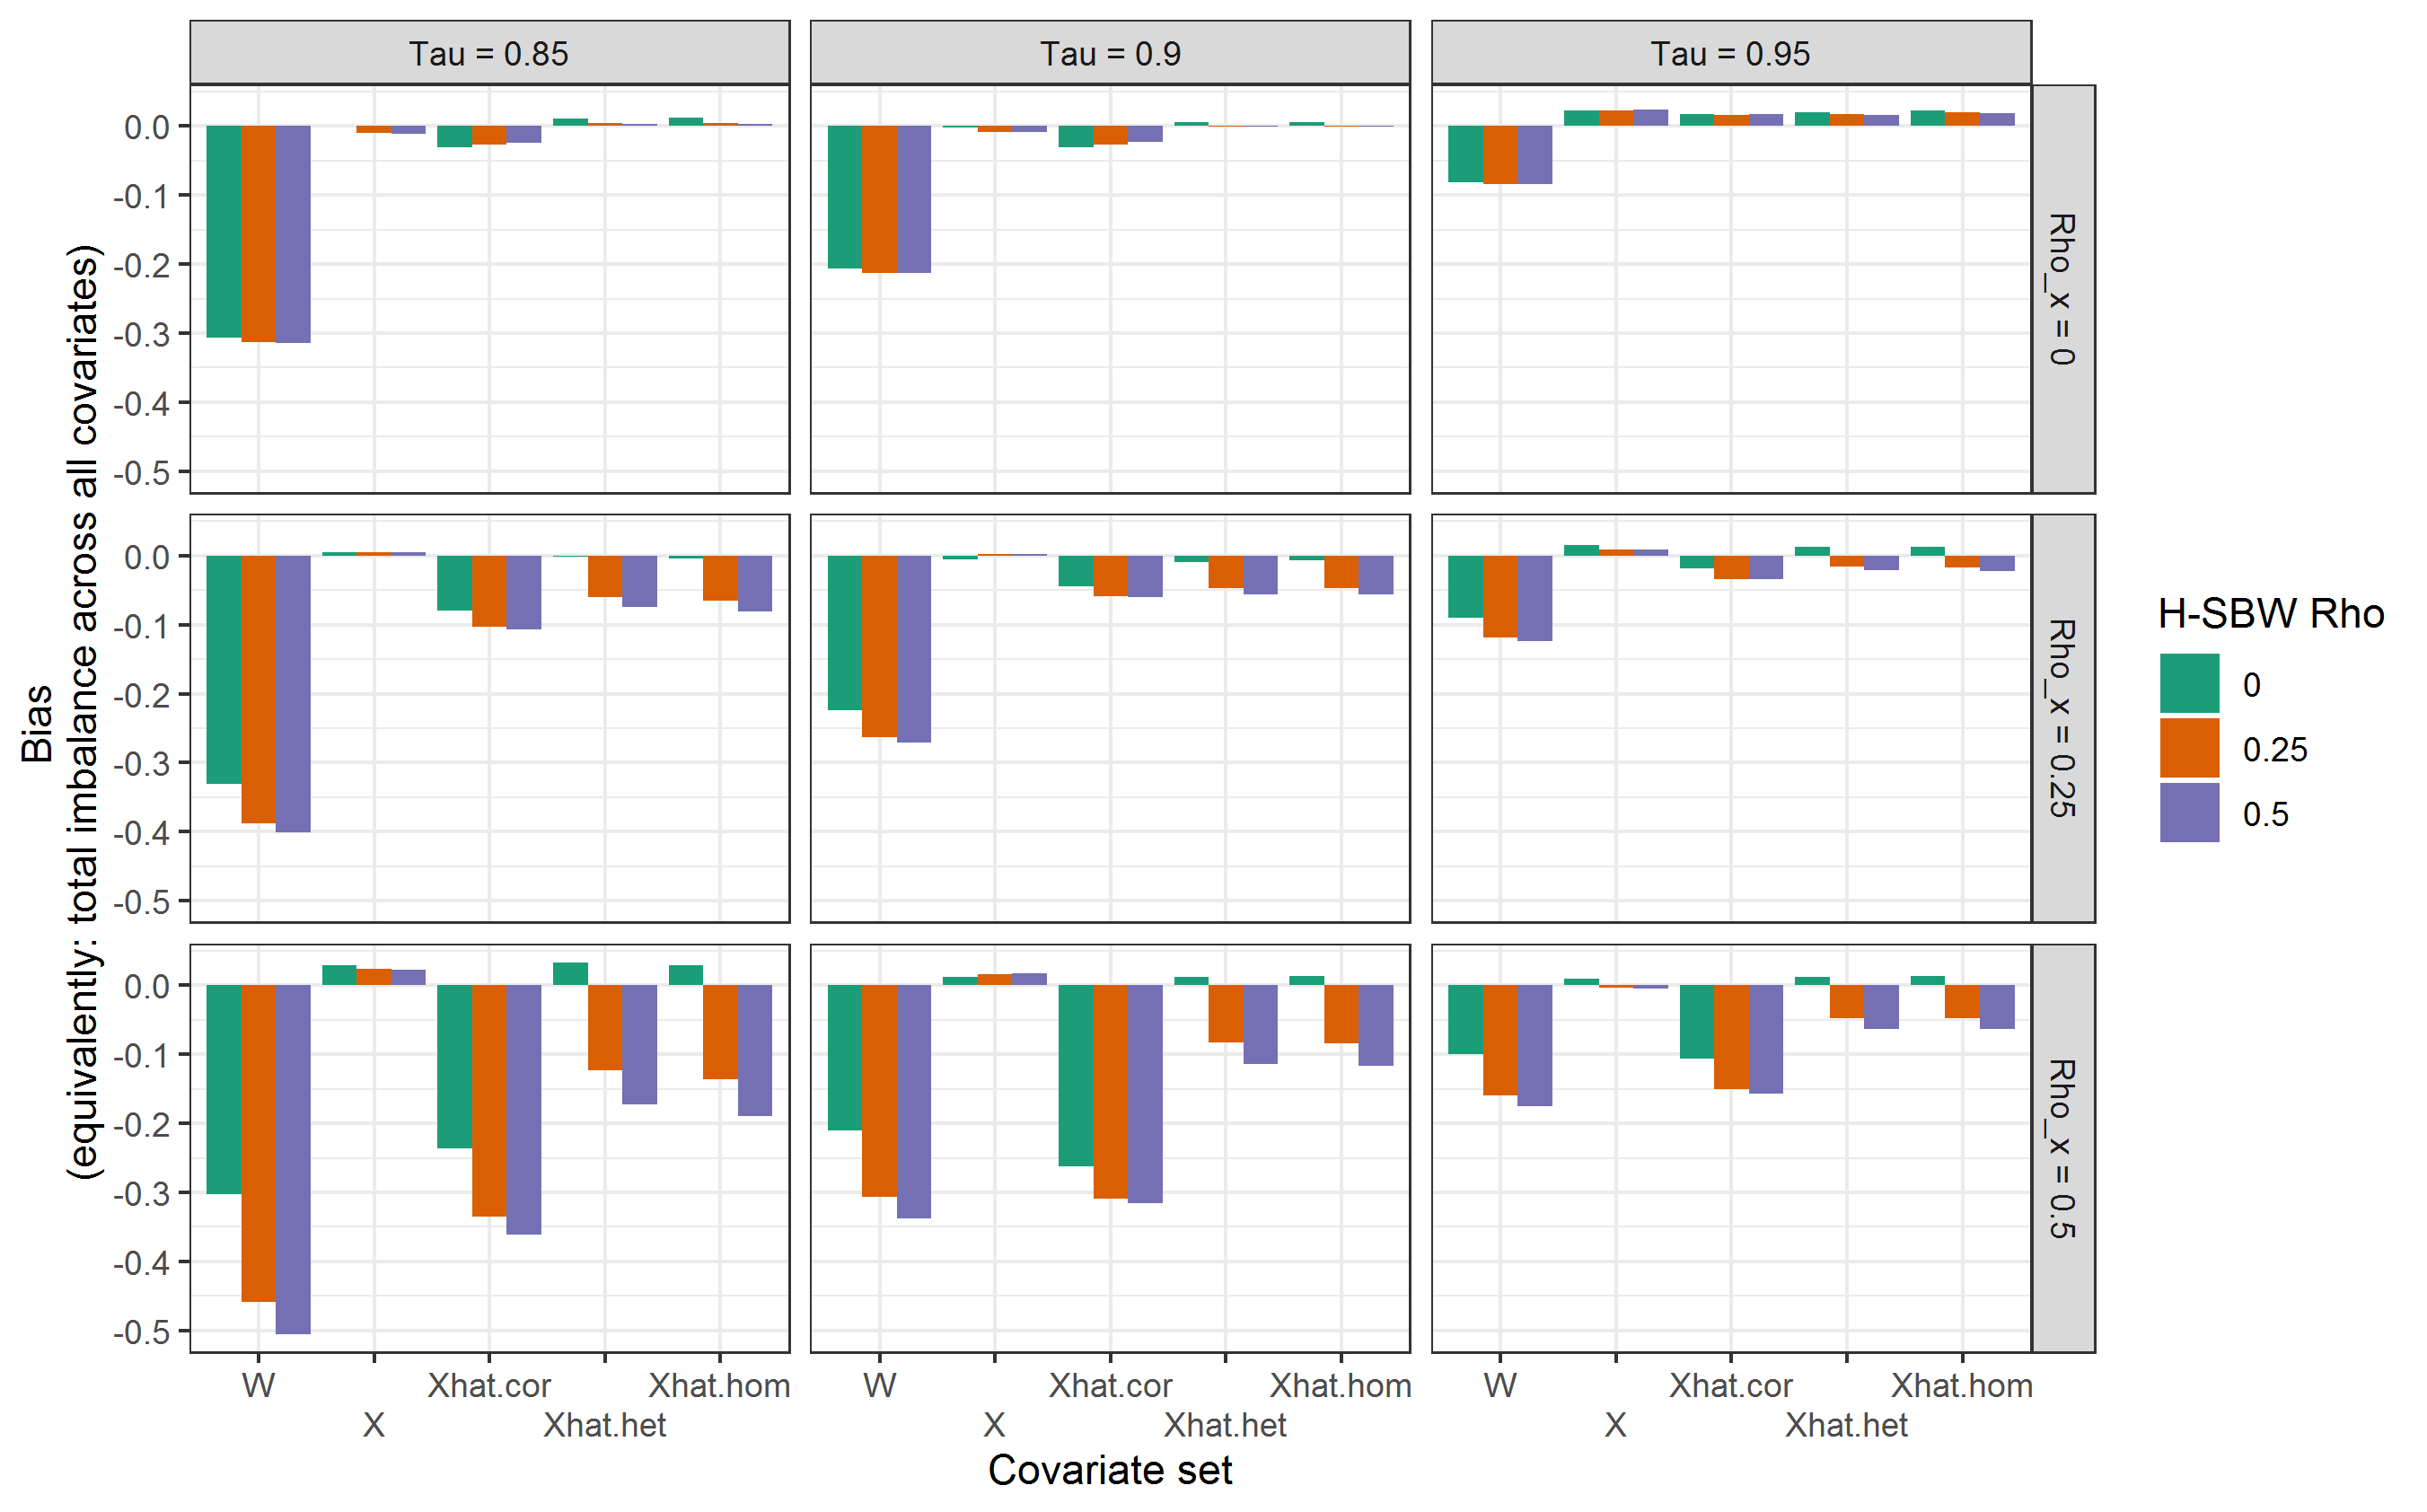
\includegraphics[scale=0.5]{01_Plots/bias-plot.png}
    \subcaption{Averaged across 500 simulations for each specification}
\end{center}
\end{figure}

All of these simulations had heterogeneous measurement. When we examine the results when the errors are homogeneous (results not displayed but available on request), we find that the estimators that balance on $\tilde{X}^{het}_{A=1}$ have a small bias even when $\tau = 0$ or $\rho = 0$. Assuming this model is correct when it is not appears to have some cost. This may help explain the worse performance we found when applying the heterogeneous adjustment to our validation study in Section~\ref{sec:results}.

We next calculate the variance our estimates across all simulations and display these results in Figure~\ref{fig:simvar}. Unsurprisingly, we find that we obtain a modest variance reduction as we increase $\rho$. Interestingly, even when $\rho$ is incorrect (assumed $0.5$ instead of $0.25$), we tend to get nearly identical improvements to $\rho = 0.25$. We also see that balancing on $\tilde{X}^{cor}_{A=1}$ can lead to a much more variable estimate, again suggesting a large cost to using this procedure given a small sample size.

\begin{figure}[H]
\begin{center}
    \caption{Simulation study: estimator variance}\label{fig:simvar}
    \label{fig:loveplotc1}
    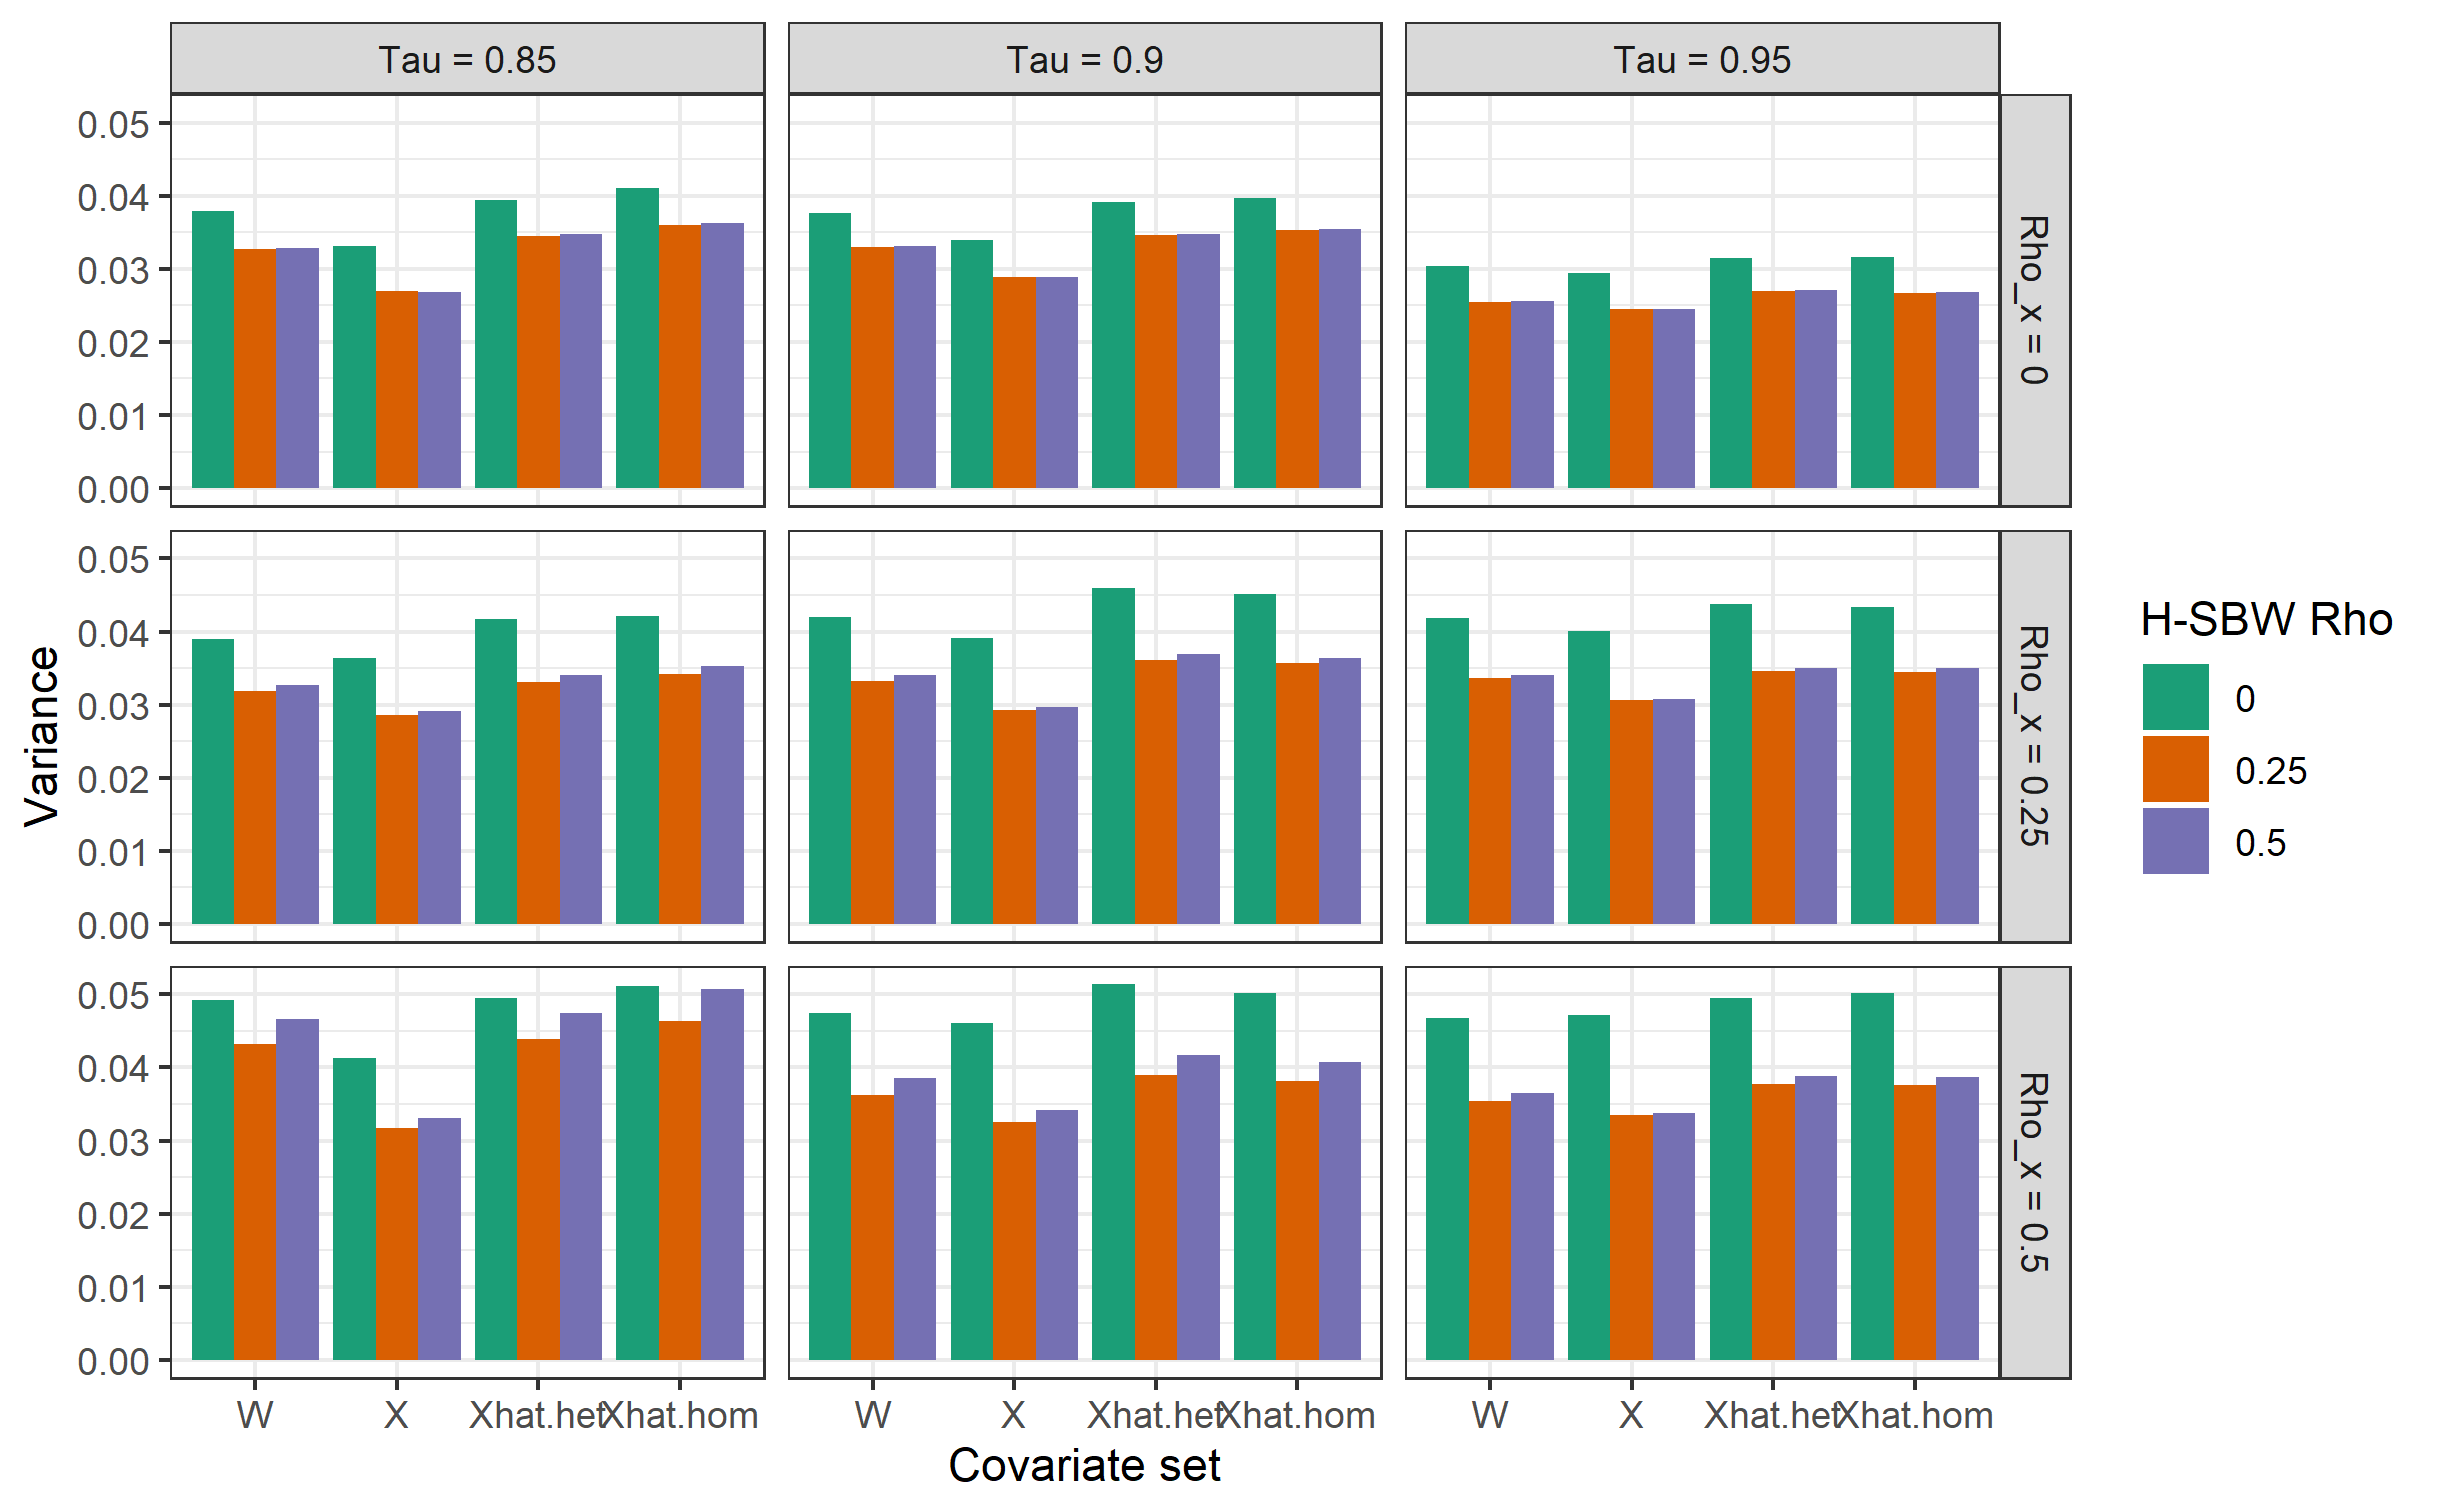
\includegraphics[scale=0.5]{01_Plots/var-plot.png}
    \subcaption{Averaged across 500 simulations for each specification}
\end{center}
\end{figure}

In Figure~\ref{fig:simmse} we display the MSE of these estimators (we remove $\tilde{X}_{A=1}^{cor}$ since we have already seen that it has poor performance relative to the other procedures considered). We find that despite the increase in bias for H-SBW with $\hat{X}_{A=1}^{hom}$ or $\hat{X}_{A=1}^{het}$, we may still find a modest MSE reduction. In particular, we see that this is more likely in regimes with low measurement error and less correlated covariates. Of course, more generally this also depends on $\rho_y$, which we have fixed here throughout: if we were to set $\rho_y = 0$, we would expect the MSE of these estimators to increase for all estimators as $\rho$ increased, even when we observe $X$. 

\begin{figure}[H]
\begin{center}
    \caption{Simulation study: estimator mean-square-error}\label{fig:simmse}
    \label{fig:loveplotc1}
    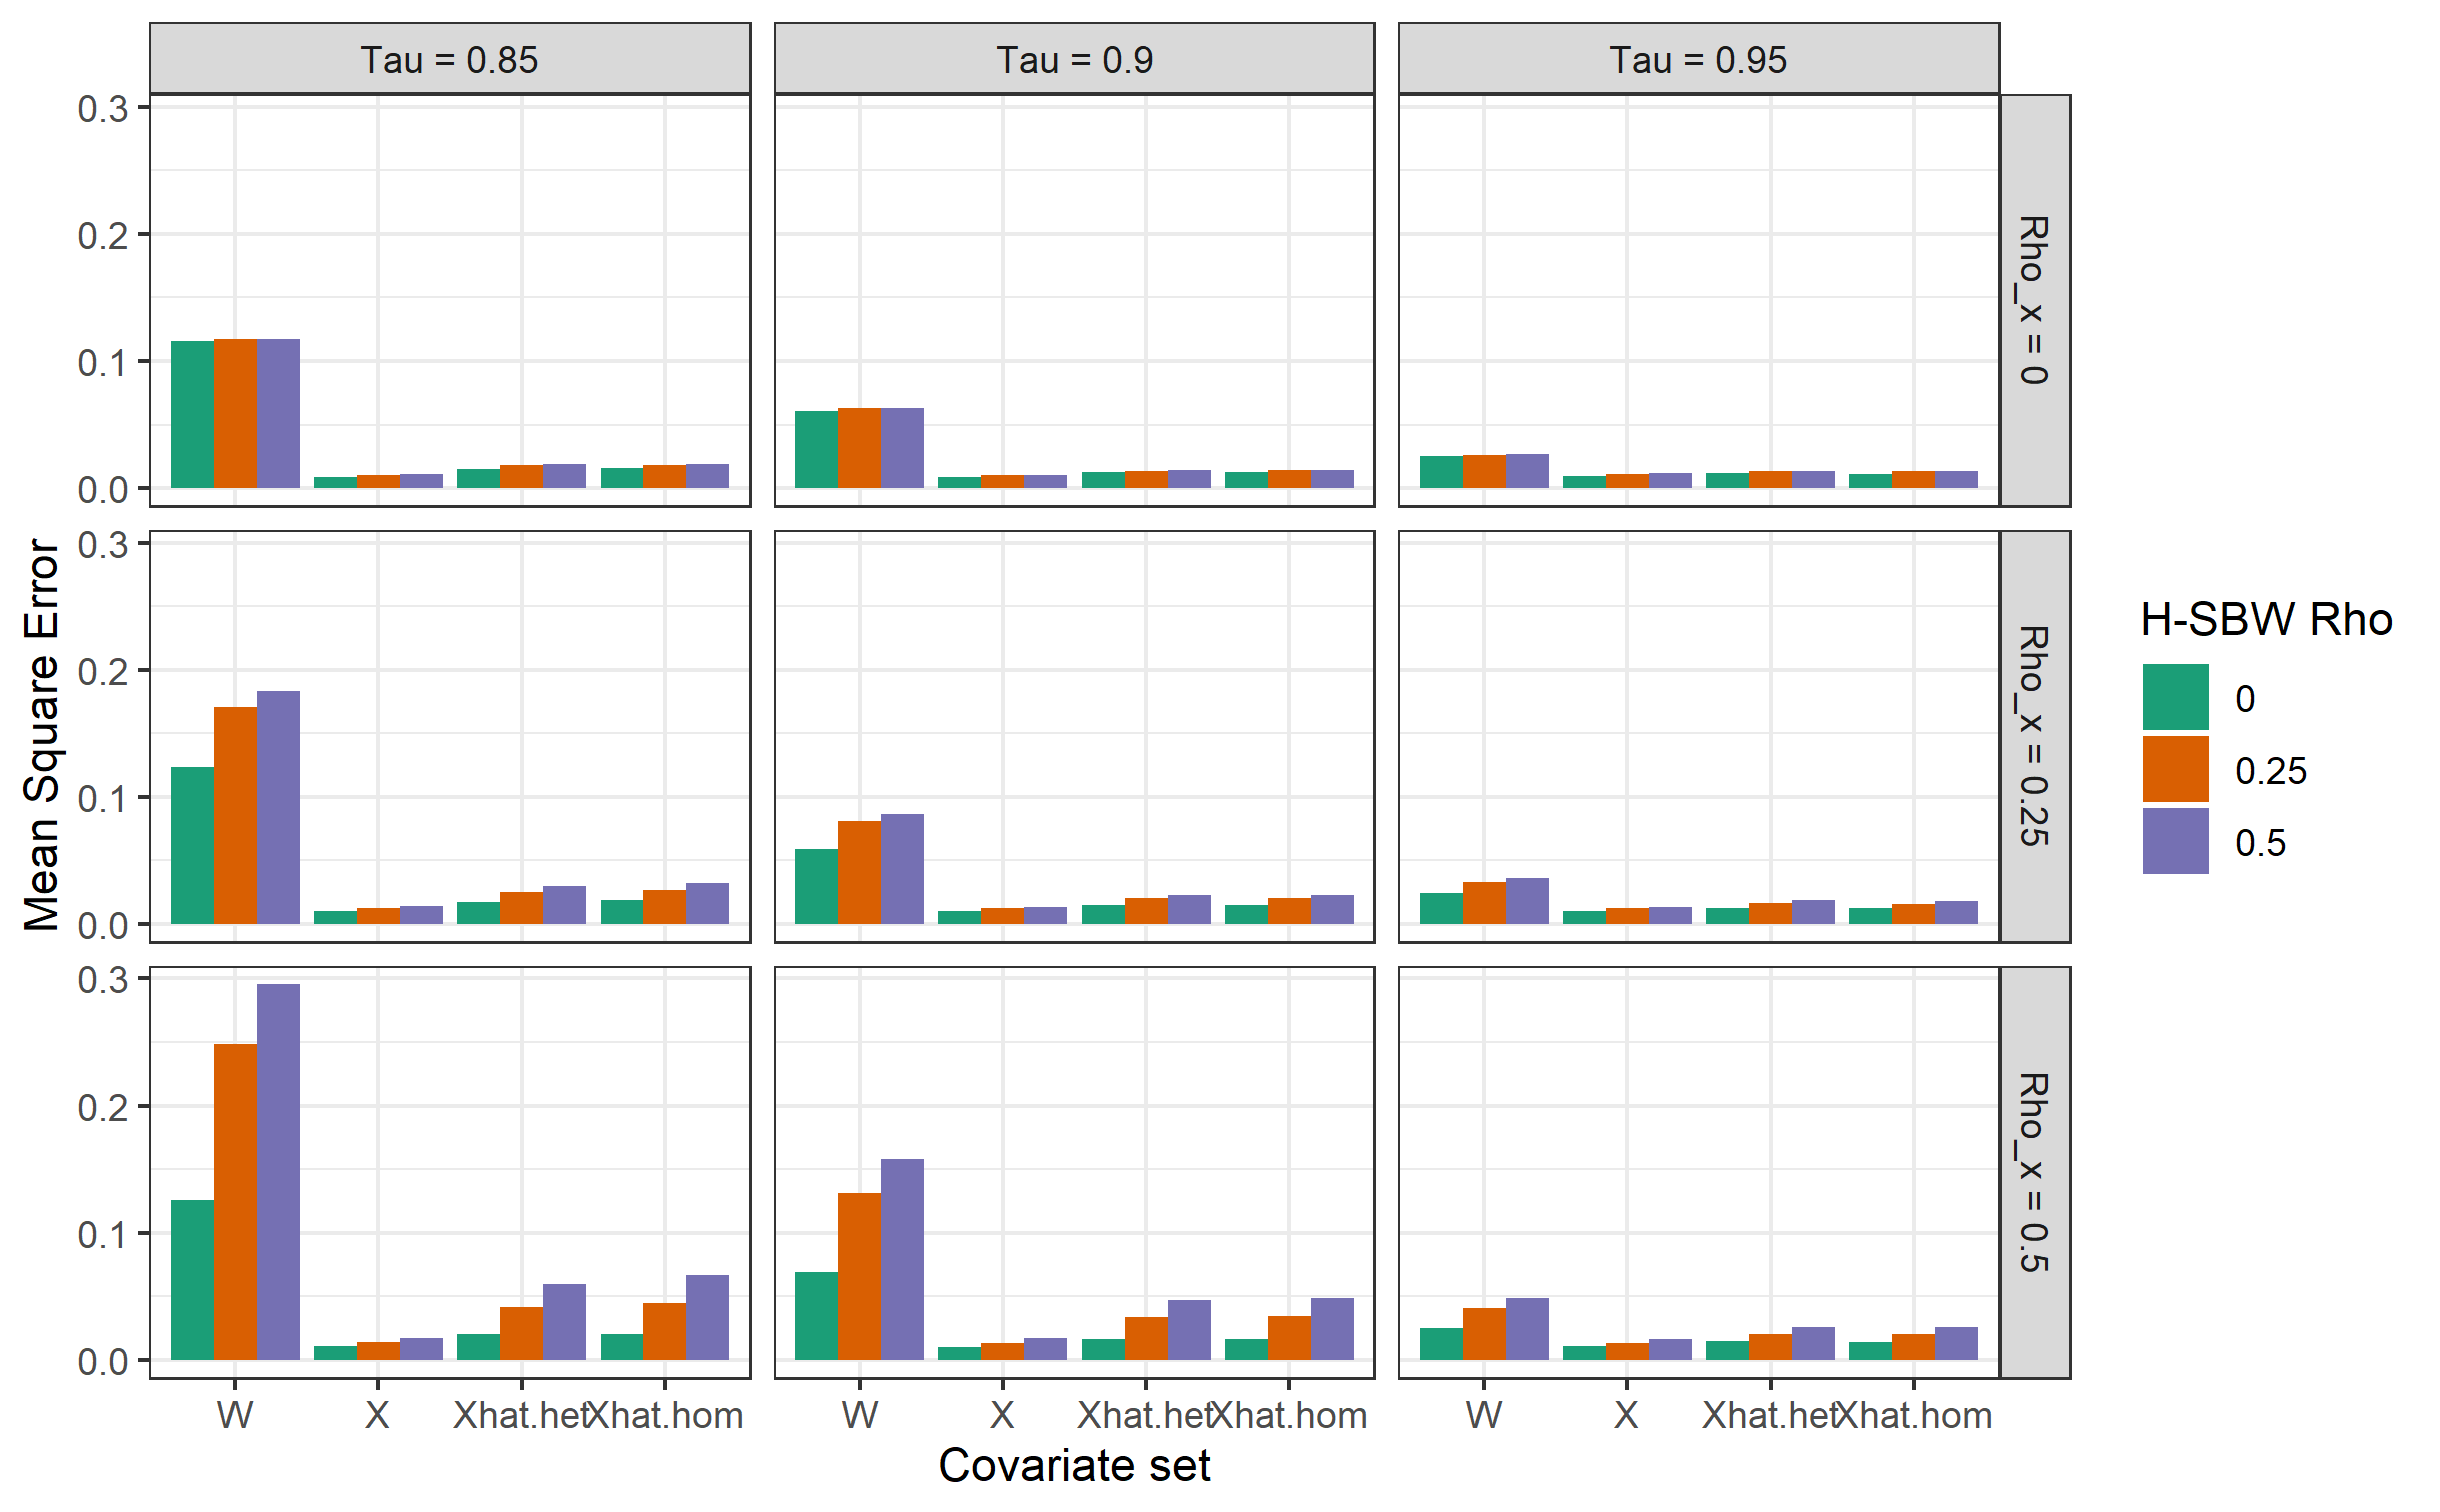
\includegraphics[scale=0.5]{01_Plots/mse-plot.png}
    \subcaption{Averaged across 500 simulations for each specification}
\end{center}
\end{figure}

Finally, we evaluate the performance of the leave-one-state-out jackknife procedure and evaluate confidence interval coverage and length. We display these results in Figures~\ref{fig:simcoverage1} and ~\ref{fig:simcoverage2}. 

We first discuss Figure~\ref{fig:simcoverage1}. When $\rho = 0$ we find that we obtain approximately nominal coverage rates across all specifications that use $X$ or some version of $\hat{X}$. However, we fail to get even close to nominal coverage rates when balancing on $W$, even when $\tau$ is quite high. We do see the performance of our estimates deteriorate as we increase $\rho_x$, even when balancing on the true covariates. We also see that our coverage rates tend to get worse for $\hat{X}^{het}$ and $\hat{X}^{hom}$ in the settings where we found the highest bias. On the other hand, we also find that our coverage rates are often quite conservative, particularly for estimators generated on $\hat{X}$. 

\begin{figure}[H]
\begin{center}
    \caption{Simulation study: jackknife coverage rates}\label{fig:simcoverage1}
    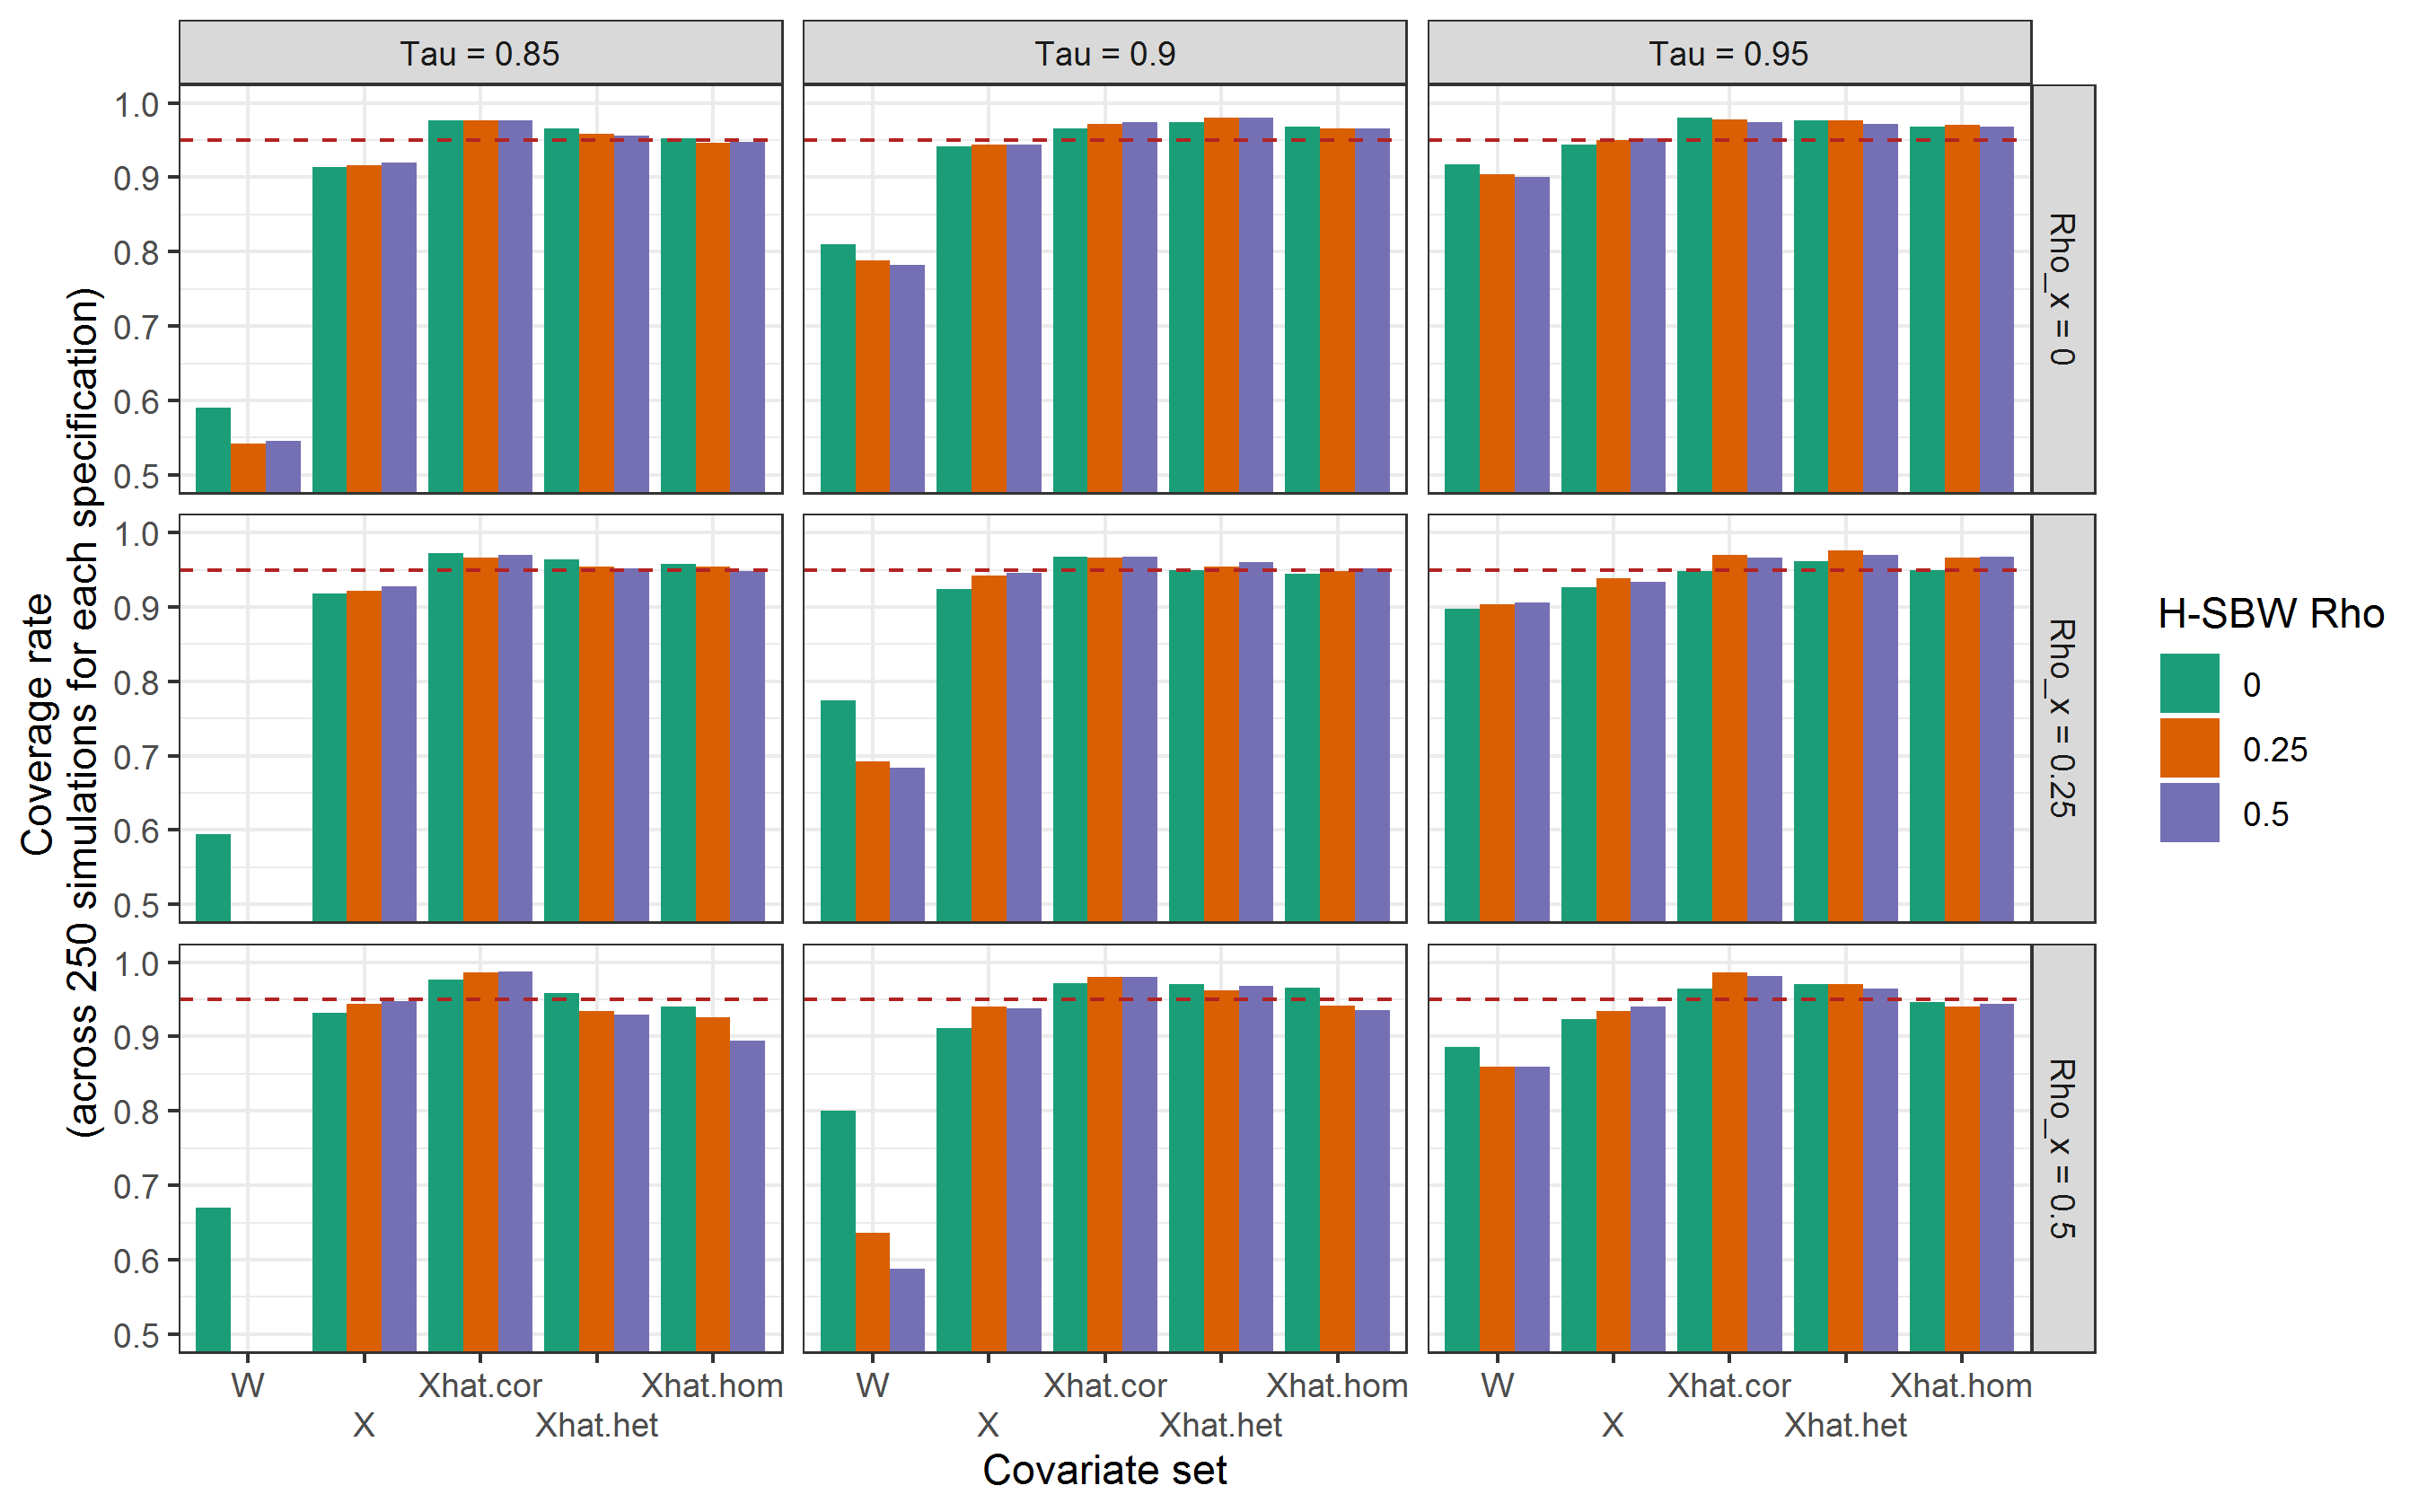
\includegraphics[scale=0.5]{01_Plots/coverage-plot-1.png}
    \subcaption{Averaged across 500 simulations for each specification}
\end{center}
\end{figure}

The figure displays one final and subtle but interesting feature: when we observe $X$, setting $\rho > 0$ appears to improve the coverage rates. We speculate this may be because H-SBW more evenly dispersing weights across states, increasing the ``effective sample size'' of the states, and thereby improving the asymptotic approximation of the variance estimates. We explore this feature more in Section~\ref{appssec:simstudyresults2} for different parameterizations of $\rho_y$. 

Finally, in Figure~\ref{fig:ciwdth} we evaluate the confidence interval lengths. As expected, we find that the H-SBW estimator is associated with lower lengths, reflecting that the estimators have decreased variability under our correlation structures. The optimal $\rho$ throughout is 0.25; however, we see that even $\rho = 0.5$ we obtain more precise inferences than when $\rho = 0$. Of course, in the context of measurement error, this also risks inducing more bias, though without measurement error this suggests benefits to using H-SBW even when our estimate of $\rho$ is a guess. All results are similar when considering homoskedastic measurement errors. 

\begin{figure}[H]\label{fig:ciwidth}
\begin{center}
    \caption{Confidence interval length}\label{fig:simcoverage2}
    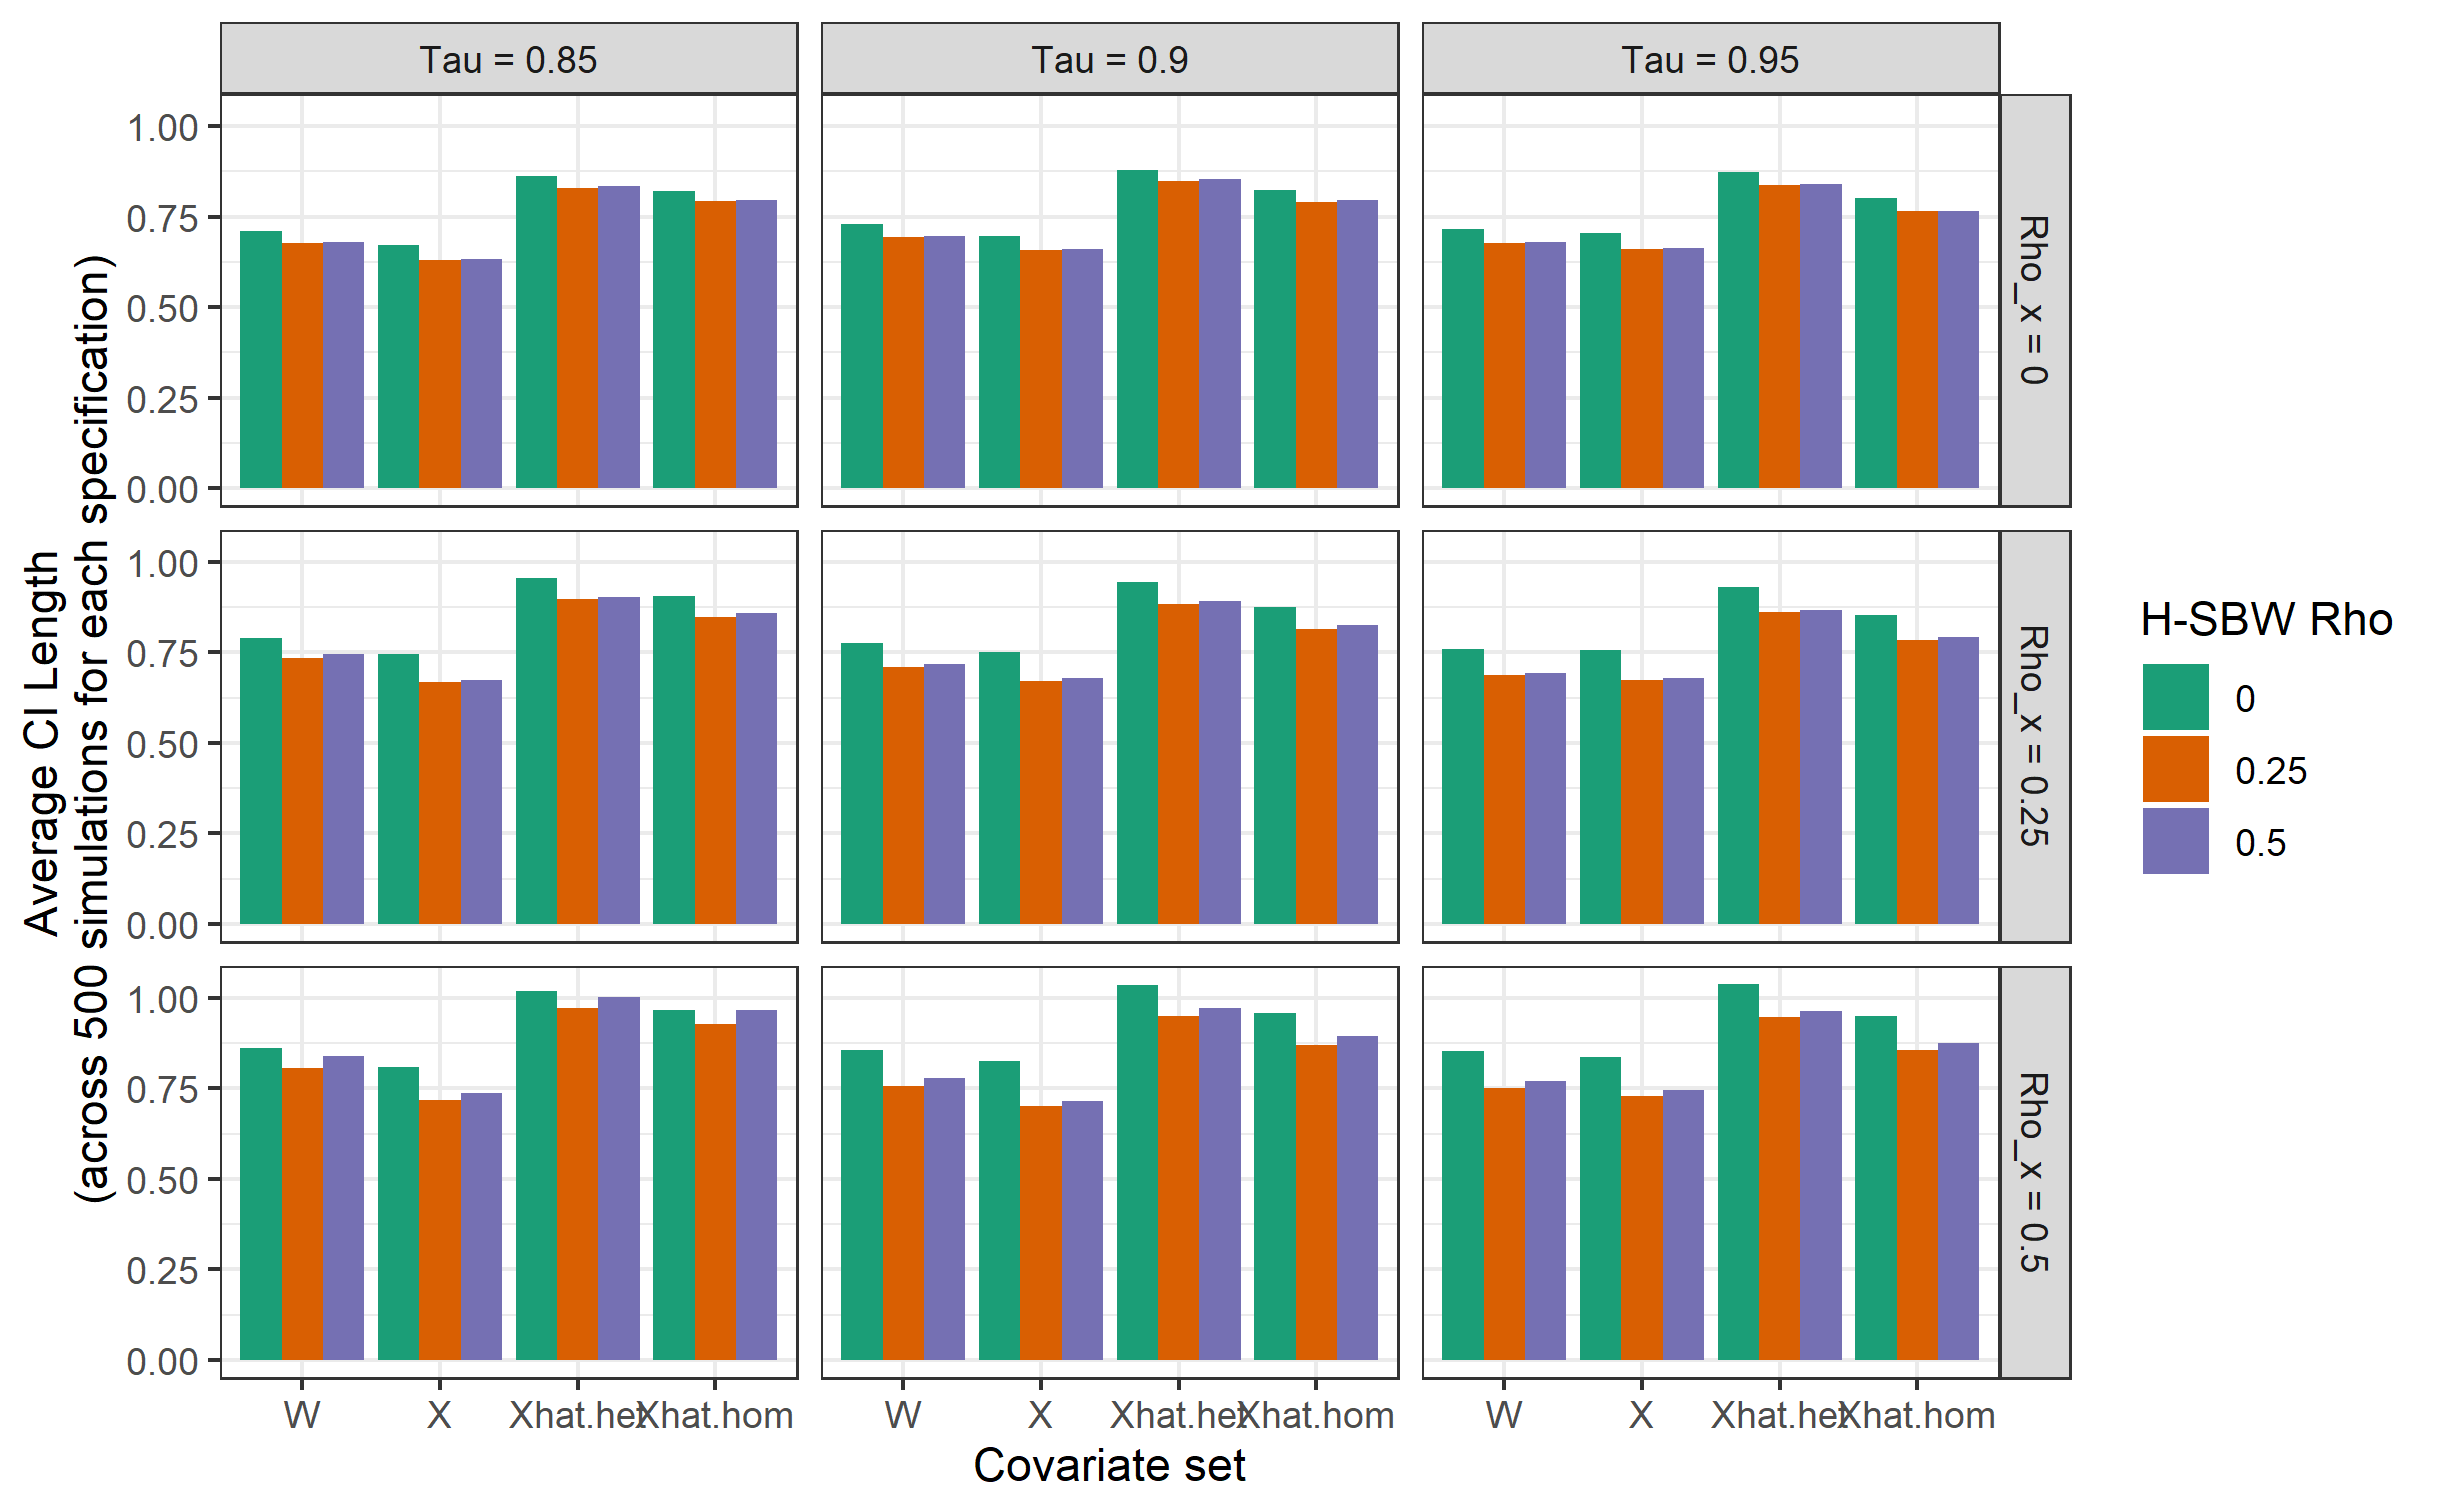
\includegraphics[scale=0.5]{01_Plots/ci-length-plot.png}
    \subcaption{Averaged across 500 simulations for each specification}
\end{center}
\end{figure}

We emphasize three takeaways from this simulation study. First, we do not find any evidence that the ``heterogeneous adjustment'' improves our estimates along any dimension, even in an ideal setting. However, this may in part reflect the distribution of sample sizes we generated, which we took to be uniform; perhaps with a different distribution these results would differ. Second, while setting $\rho > 0$ can increase the bias of our estimates in the context of measurement error, the bias is generally small relative to the bias of balancing on the noisy covariate measurements $W$. Even so, MSE improvements using H-SBW are still possible relative to SBW if we assume some non-negligible state-level random effect and relatively small measurement error. Third, accounting for the correlation in the data when using H-SBW and the data are measured with error may not be worth it given a small sample of states, despite the improved theoretic properties. This simulation study assumes throughout that we know the true data generating model for the outcome, and that are data are Gaussian. This study complements our validation study in Section~\ref{sec:results}, which has more direct bearing on understanding how these estimators might perform in our application.

\subsubsection{Additional results}\label{appssec:simstudyresults2}

In this subsection we demonstrate two additional results: first, that the correlated adjustment procedure proposed in Appendix~\ref{app:adjustmentdetails} is consistent as $m \to \infty$. Second, we consider confidence interval coverage for H-SBW with known covariates $X$, setting $m = 25$ but varying $\rho_y$, and demonstrate that H-SBW can improve the corresponding coverage rates relative to SBW when using the leave-one-state-out jackknife. 

\end{document}
 